\documentclass{mscThesis}
\usepackage{amsmath}
\usepackage{graphicx} 
\usepackage{bm} % bold-face greek characters
\usepackage{color} % font colors
\usepackage{subfigure}
\usepackage{algorithm}
\usepackage{algpseudocode}
\usepackage{multirow}
%\usepackage{caption}
%
\providecommand{\AddToShipoutPictureBG}{\AddToShipoutPicture}
\providecommand{\AddToShipoutPicture}{\AddToShipoutPictureBG}
\providecommand{\AtBeginShipoutUpperLeftForeground}{\AtBeginShipoutUpperLeft}
\providecommand{\AtBeginShipoutUpperLeft}{\AtBeginShipoutUpperLeftForeground}
%
% use the option 'nosignatures' to turn off the signatures page
%
%
% Thesis data
\mscDepartment{Delft Center for Systems and Control (\textsmaller{DCSC})}%
\mscProgram{Systems and Control}% or {Mechanical Engineering}
\mscFaculty{Mechanical, Maritime and Materials Engineering (3mE)}%
\mscName{Thijs Ramakers}%
\mscDate{\today}%
\mscTitle{Memory-based Modeling and \\ Prioritized Sweeping in \\ Reinforcement Learning}%
%\mscSubTitle{Optional Subtitle}%
\mscKeyWords{Thesis, MSc, Reinforcement Learning, RL, Local Linear Regression, LLR, Prioritized Sweeping, PS}% only used in PDF properties
%\mscCoverPicture{Figures/coverpicture}% to place a picture on the back of the cover page
%
%
% Third party options (create text/logo on the copywrite page)
%\mscThirdPartyText{The work in this thesis was supported by Aquaduct Swimming Supplies Incorporated. Their cooperation is hereby gratefully acknowledged.}
%\mscThirdPartyLogo{STYLESTUFF/EXAMPLELOGO}
% NOTE: on the title page only the TU Delft logo is permitted.
%
%
% The examination committee
\mscSupervisorOne{Prof.dr. R. Babu\v{s}ka}
\mscSupervisorTwo{Dr.ir. G. Lopes}
\mscSupervisorThree{Ir. E. Schuitema}
\mscReaderOne{Dr.ir. M. Wisse}
%\mscReaderOne{prof.dr.ir. R. Babu\v{s}ka}
%\mscReaderTwo{dr.ir. G. Lopes}
%\mscReaderThree{MSc. E. Schuitema}
%\mscReaderFour{P. Jonker}
%
% Finalize the thesis data
\setThesisInfo
%
% Use \includeonly{} to build only certain parts of your thesis
%\includeonly{introduction, real_chapter, empty_chapter, long_chapter}%
%
%\setcounter{tocdepth}{3} % TOC depth
\begin{document}
%
%========================== Front matter ======================================
\frontmatter %
%
% Make the cover page and hell of a lot of title pages
\maketitle
%
\chapter{Abstract}

% Title: Memory-based Modeling and Prioritized Sweeping in Reinforcement Learning

% Final thesis

\acf{RL} is a popular method in machine learning. In RL, an agent learns a policy by observing state-transitions and receiving feedback in the form of a reward signal. The learning problem can be solved by interaction with the system only, without prior knowledge of that system. However, real-time learning from interaction with the system only, leads to slow learning as every time-interval can only be used to observe a single state-transition. Learning can be accelerated by using a Dyna-style algorithm. This approach learns from interaction with the real system and a model of that system simultaneously. Our research investigates two aspects of this method: Building a model during learning and implementing this model into the learning algorithm.

We use a memory-based modeling method called \acf{LLR} to build a state-transition model during the learning process. It is expected that the quality of the model increases as the number of observed state-transitions increases. To assess the quality of the modeled state-transitions we introduce prediction intervals. We show that LLR is able to model various systems, including a complex humanoid robot.

The \acs{LLR} model was added to the learning algorithm to generate more state-transitions for the agent to learn from. We show that an increasing number of experiences leads to faster learning. We introduce \acf{PS} and \acf{LA Dyna} as possibilities to use the model more efficiently. We show how prediction intervals can be used to increase the performance of the various algorithms. The learning algorithms were compared using an inverted pendulum simulation, which had to learn a swing-up control task.



% Literature Colloquium
%Reinforcement Learning (RL) is a popular learning method. Learning is done by an agent that chooses actions and learns by observing state transitions and receiving reward for those transitions. Different basic solution methods exist that are capable of solving a RL task. Some of these methods rely on the availability of a model of the system, some learn without an explicit model and a third class builds a model during the learning process. These solution methods have all proven to be applicable, but only to relatively simple problems. In many applications however, large continuous state-spaces lead to a problem known as the curse of dimensionality. For these problems, learning becomes very slow or even impossible. An example of such a difficult learning task is learning a humanoid robot to walk. The robot learns from direct interaction with the environment, which is called on-line learning. The large number of continuous variables makes the application of RL a big challenge for such problems.
%In this presentation model-learning methods for systems with large, continuous state-spaces will be discussed. The focus will be on dealing with continuous variables, storing the learned model efficiently and increasing the learning speed.

% Introductory Colloquium
%Reinforcement Learning (RL) is a popular learning method. Learning is done by an agent that chooses actions and learns by observing state transitions and receiving reward for those transitions. Different basic solution methods exist that are capable of solving a RL task. Some of these methods rely on the availability of a model of the system, some learn without an explicit model and a third class builds a model during the learning process. These solution methods have all proven to be applicable, but only to relatively simple problems. In many applications however, large continuous state-spaces lead to a problem known as the curse of dimensionality. For these problems, learning becomes very slow or even impossible.
%A technique that could increase the learning speed is Prioritized Sweeping. This method relies on building a state-transition model during the learning process and then using that model to generate more experiences for the agent to learn from. This project will try to develop methods to use Prioritized Sweeping and eventually apply them on a humanoid robot setup.

%
% table of contents, (\toc of \toclof of \tocloflot )
\tocloflot
%
%
%%%
% Preface
\chapter{Preface}

According to \textsc{WikipediA}, a preface (pronounced ``\emph{preffus}'') is an introduction to a book written by the author of the book. In this preface I can discuss the interesting story of how this thesis came into being. 

This is document is a part of my Master of Science graduation thesis. The idea of doing my thesis on this subject came after a discussion with my good friends Tweedledum and Tweedledee\ldots


\chapter{Acknowledgments}

Just like reinforcement learning, scientific research has a trial-and-error nature. The research for this master's thesis was no exception. Although a project plan was made at the start, the obtained results forced the project in certain directions that were not always foreseen in the beginning. Every choice made during research led to new questions and new options. 

I would like to thank my supervisors for providing lots of ideas and suggestions, while allowing me the freedom to make my own choices in the end. I owe many thanks to Prof.dr. Robert Babu\v{s}ka for his broad knowledge, numerous ideas and useful feedback. I would also like to thank my daily supervisors dr.ir. Gabriel Lopes, for his useful suggestions and enthusiasm, and ir. Erik Schuitema, for his advice and for placing this research in a practical context.

Finally, I would like to thank my family, Margot and friends. Although they could not give me answers to my research questions, they did provide the support that was needed for finalizing my master.

Delft, University of Technology \hfill \mscname \\
\mscdate
%%%
% Dedication page. 
\cleardoublepage
\thispagestyle{empty}
\vspace*{\stretch{1}}

% Put your own motto here, or dedicate your work to your Mom or whatever...
\begin{quote}
\noindent``In the future, airplanes will be flown by a dog and a pilot. And the dog's job will be to make sure that if the pilot tries to touch any of the buttons, the dog bites him.''
	
--- \emph{Scott Adams}
\end{quote}

\vspace{\stretch{3}}
\clearemptydoublepage
%
%========================== Main matter ======================================
\mainmatter
%
%%%
% Introduction
\chapter{Introduction} \label{chap::intro}

This is a \LaTeX\ thesis and this is Chapter\ \ref{chap::intro}. 

\section{About \texorpdfstring{\LaTeX}{LaTeX}}

\LaTeX\ is a document preparation system for the \TeX\ typesetting program. It offers programmable desktop publishing features and extensive facilities for automating most aspects of typesetting and desktop publishing, including numbering and cross-referencing, tables and figures, page layout, bibliographies, and much more. 

\LaTeX\ was originally written in 1984 by Leslie Lamport and has become the dominant method for using \TeX; few people write in plain \TeX\ anymore. The current version is \LaTeXe.

If you want to know more about \LaTeX\ you better read \cite{texbook}.\index{LaTeX} 

 
\section{About Acronyms}

This section contains an acronym of the \ac{DCSC}. The \ac{DCSC} is our department within the faculty of \ac{3mE} at \ac{TU}. \index{acronym}

Acronyms are automatically listed in the Glossary in the back of this thesis. You have to define acronyms in \texttt{glossary.tex} using \verb"\acro{ACRONYM}{Full text}". You print an acronym by using the command \verb"\ac{...}". You can always force a full, long or short printout by using \verb"\acf{...}", \verb"\acl{...}" or \verb"\acs{...}" respectively. 

\begin{itemize}
	\item \verb"\acf{DCSC}": \acf{DCSC};
	\item \verb"\acl{DCSC}": \acl{DCSC};
	\item \verb"\acs{DCSC}": \acs{DCSC}.
\end{itemize}

\section{About the Nomenclature}

When you use symbols in your thesis -- as you probably will -- you can put them into the nomenclature listing (List of Symbols) at the back of your thesis. \tabref{tab:nomencl} shows the \LaTeX\ commands you need.\index{nomenclature}

\begin{table}%
	\centering
	\caption{Nomenclature codes}
	\label{tab:nomencl}
	\begin{tabular}{llcl}
		\toprule
		Code & Usage & Example\\
		\midrule
		\verb"\gsymb{}" & Greek symbols & \gsymb{$\gamma$}{Path Angle}\\
		\verb"\lsymb{}" & Letter symbols & \lsymb{$H(s)$}{Transfer function}\\
		\verb"\supers{}" & Superscript symbols & \supers{max}{Maximum} &\emph{only printed in the List of Symbols} \\
		\verb"\subs{}" & Subscript symbols & \subs{min}{Minimum} &\emph{only printed in the List of Symbols}\\
		\verb"\others{}" & Other symbols & \others{[kts]}{Knots} \others{$^{\circ}$, [deg]}{Degrees} &\emph{only printed in the List of Symbols}\\
		\bottomrule
	\end{tabular}
\end{table}


%%%
% A Real Chapter
\chapter{First Real Chapter}

This is real chapter for \ac{DCSC}, ok? We will use it as a demo for the different headings you can use to structure your text.


\section{First Section}

This is the section. Referring to equations, figures and tables can easily be done by the commands \verb"\eqnref{}", \verb"\figref{}" and \verb"\tabref{}".

\begin{equation}\label{eq:First}
	H(s) = \frac{1}{s+2}
\end{equation}

You see? Refer to equations like this \eqnref{eq:First}.


\subsection{The first subsection}

Subsections are the last type of sectioning that is numbered. 


\subsubsection[Subsection Short Title]{The first sub-subsection with a very very very long title, but in the Table of Contents one can only see the short title}

Quick! Check the Table of Contents! Nice, ain't it?\index{Nice}


\paragraph{A paragraph title}

Subdividing your text in sections and paragraphs automatically makes it nice and structured.
		
\include{Chapter_Introduction}
%\include{Chapter_Problem_Statement}
%
\include{Chapter_RL}
\chapter{Memory-based modeling}\label{chap:Modeling}

 
\section{Introduction}\label{sec:LLR-introduction}
As described in Section \ref{sec:RL-Dyna_style_methods}, using a state-transition model of a system can be useful in speeding up the learning process. Typically, such a model is not available for real systems. Hence, such a model has to be constructed. In this work, we focus on building a model during the learning process\footnote{In literature, some authors use the term model 'learning' to refer to the construction of a model. In this thesis, the term \emph{learning} will be used for reinforcement learning methods only. The term \emph{building} will be used to refer to the construction of the model. This in order to emphasize the difference between the reinforcement learning methods and modeling methods.}. The only data available for building a model, are the transitions that are experienced by the system during learning. This approach has the virtue that the model can be adapted to possible changes in the system dynamics. This is an advantage for autonomously operating systems. Furthermore, there is no need for separate identification experiments (which could be difficult or expensive in real-world situations). Building a model using identification experiments and then applying them in a \ac{RL} setting is also possible and has been done successfully in the past \cite{Ng:04}, \cite{Bakker:03}, \cite{AtkesonSchaal:97}. 
% Because the model is being build during learning, the model-building method should be able to estimate a model from relatively few observations. 
% We always have to keep in mind that these methods will be used in online experiments (with real-time interaction with noisy data)

In this chapter we argue that a memory-based approach to building a state-transition model is interesting in a \ac{RL} setting. The method used is \ac{LLR}. This method assumes the state-transition model to be locally linear. Upon a query input, a nearest neighbor search is carried out and a linear model is fitted through the obtained set of nearest neighbors. The fitted model is used to estimate an output.

This chapter is organized as follows. First an introduction to memory-based modeling is given in Section \ref{sec:LLR-memory-based modeling}. In Section \ref{sec:LLR-local linear regression} the Local Linear Regression method is introduced and some statistical methods are introduced. Finally Section \ref{sec:LLR-results} presents the results obtained with three different setups.




\section{Memory-based modeling}\label{sec:LLR-memory-based modeling}
Memory-based modeling is a class of modeling methods that memorizes all samples and delays the estimation of a model and output until a query is made. Since modeling is deferred to the moment a query is made, this approach is also known as lazy-learning. Its opposite is eager-learning, which adjusts the model for every new sample that is obtained. Eager-learning methods (such as artificial neural networks) assume that a global parametric model structure is known and adjust its parameters according to some error-measure. In general, eager-learning methods discard the data they were trained on after the parameters have been tuned.

%In general, memory-based methods do not use the full set of stored samples to estimate a model. Only the subset of samples that are very similar to the query input are used in the estimation. In this way, a local model is built that is only valid in the vicinity of the query input. 

In this research, the stored samples are state-transitions $(\mathbf{x}_t,\mathbf{u}_t)\rightarrow \mathbf{x}_{t+1}$, the input-query $(\mathbf{x}_q,\mathbf{u}_q)=(\mathbf{x}_t,\mathbf{u}_t)$ is a state-action pair at time $t$ and the estimated output $\hat{\mathbf{x}}_{t+1}$ is the resulting next state. In order to avoid confusion and to comply with the usual terminology in modeling, we will use the terms (query) \emph{input} for $(\mathbf{x}_t,\mathbf{u}_t)$ and \emph{output} for $\mathbf{x}_{t+1}$, instead of referring to states explicitly.


\paragraph{Advantages} Memory-based modeling is also known as nonparametric modeling, as no global (parametric) model structure is used. Instead, for every query a model is estimated that is valid in the vicinity of the query input. In general, one uses only samples close to the query input to estimate the model. This can lead to a model that is able to estimate local nonlinearities very accurately. When enough samples are available around a query point, estimations can be accurate locally, even if large parts of the state-space have rarely been visited. Therefore, memory-based modeling can lead to accurate estimates after relatively few observation. This is very useful in a \ac{RL} setting, in which an accurate model is required although the number of observed state-transitions might be limited.

A second advantage is that no detailed knowledge about the system dynamics is needed to obtain good quality estimates. Obtaining a representative parametric model of a system might be difficult and the obtained global model might not represent local nonlinearities accurately. Memory-based models can even be used if the knowledge about the system to model is very limited. This makes memory-based modeling useful for a wide range of applications. This is an advantage for a \ac{RL} agent that possibly has no a priori knowledge about the environment.

Compared to eager-learning, memory-based learning seems to be favorable in a real-time experiment in which new samples are obtained continuously. Incorporating new samples in memory-based methods is straightforward. It only involves storing the new sample. In an eager-learning method, incorporating new samples means re-tuning the model parameters. This typically involves some iterative search for nonlinear models. If the tuning of the parametric model is very expensive, a memory-based approach might be more favorable.

\paragraph{Disadvantages} Estimating a model solely based on stored samples also has disadvantages. The main disadvantage is its sensitivity to noise. Since no model-structure is imposed on the data, noisy data or outliers can lead to locally inaccurate estimates. However, we can use several statistical tools to cope with noise and faulty data in order to increase the accuracy and reliability of the estimation. 

Another disadvantage of memory-based methods is the need to store all samples. This leads to two problems. First, many observed state-transitions lead to a large dataset which requires large amounts of memory to store. A second problem is that the estimation of an output can become computationally heavy since the estimation is possibly based on all stored samples and has to be re-calculated for every input query. For these reasons, memory-based modeling methods in real-time applications need to have some sort of memory management in order to prevent the number of samples in the memory to become too high. The most basic form of memory management is limiting the number of samples that are stored in the memory by replacing the oldest samples with new ones once a memory limit is reached. This approach is also logical when the system dynamics gradually change in time.
%More advanced management strategies exist \textcolor{red}{[REF]}, but these will not be considered in this work.










\section{Local Linear Regression}\label{sec:LLR-local linear regression}
In this section we will introduce the \ac{LLR} method that will be used throughout this report. \ac{LLR} is a memory-based modeling method that fits a linear model to a set of data points. These points are a subset of all the stored points and are selected according to their similarity to a query input (see \figref{fig:LLR-LLRschematic}). Typically a vector norm is used as a similarity measure, which is generally called a distance measure. The first step is to select the subset of the memory data that is closest to the query input. This search is called a \lsymb{$K$}{Number of nearest neighbors} nearest neighbors search, as the $K$ nearest samples are selected. This aspect of the method will be discussed first. The second step is fitting a linear model to the set of nearest neighbors, which will be discussed thereafter. In the last part of this section, several methods from the field of statistics will be used to assess the quality of the estimated model. 

\begin{figure}[htbp]
	\centering
		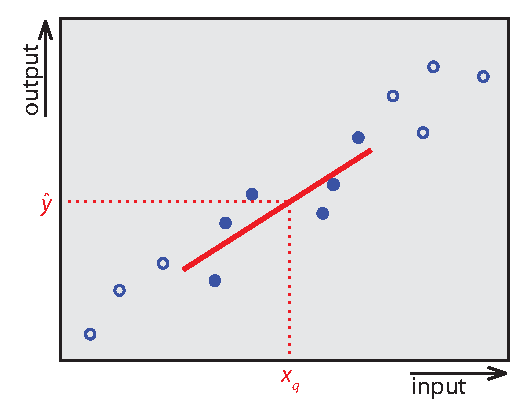
\includegraphics[width=.5\textwidth]{img/LLR_schematic2}
	\caption[\acs{LLR} on set of points]{\acs{LLR} on a set of data points. Out of a set of 13 samples (circles), a subset of 6 nearest neighbors (solid circles) is selected that are closest to the query input $x_q$. The estimated output $\hat{y}$ is found by fitting a linear model through the nearest neighbors and evaluating the obtained model for $x=x_q$.}
	\label{fig:LLR-LLRschematic}
\end{figure}

\paragraph{Alternatives} In this work we fit a linear model to the set of nearest neighbors. Linear regression (Section \ref{sec:LLR-linear regression}) is a computationally expensive step. Other options to obtain an estimate of the output are also possible. The easiest option is to simply use the output of the nearest neighbor as an estimate of the output. Also the average output of the $K$ nearest neighbors could be used as an estimate for the output. Our main reason for estimating a linear model is to reduce the influence of noise and thereby improving the estimation accuracy. In Section \ref{sec:LLR-two link manipulator} we compare \ac{LLR} with the nearest neighbor and $K$ nearest neighbors approaches. 

A more sophisticated memory-based method is \ac{LWR} \cite{SchaalAtkeson:94}. This method can improve the estimation quality compared to \ac{LLR} by introducing two types of weights. The first is a weighted distance measure which increases the influence of certain state-variables in the distance metric. The second type is a weighted linear regression procedure that increases the influence of nearby samples in the linear regression. This method is more complex than \ac{LLR} and introduces more tuning parameters compared to \ac{LLR}. The statistical results derived in this section also hold - apart from a weighting factor - for \ac{LWR}. Although it is not clear how the experimental results would be influenced. However, \ac{LWR} could be used as a good alternative to \ac{LLR} if the accuracy of the model would need to be increased.


\subsection{Nearest neighbors search}\label{sec:LLR-nearest neighbors search}
As mentioned, the first step in the \ac{LLR} algorithm is searching the memory for the set of nearest neighbors according to some distance metric $D$. The number of neighbors to be returned is $K$. The distance metric can be chosen freely, but is generally assumed to be a mathematical vector norm. We used an unweighted vector norm. Preliminary experiments showed little difference between different norms. In our experiments we have used the 1-norm (or Manhattan norm), which gave slightly better results:
$$
 D(\mathbf{a},\mathbf{b}) = \left\| \mathbf{a}-\mathbf{b} \right\|_1 = \sum_{i=1}^{k}{\left| a_i - b_i \right|}
$$
Where the $i$th component of the vector $\mathbf{a}$ is denoted by $a_i$. The dimension of the samples is \lsymb{$k$}{Dimension of a sample}. In its simplest implementation, a nearest neighbors search is composed of the following steps:
\begin{enumerate}
	\item Calculate the distance of the query point to every sample in the memory
	\item Sort the samples according to their distance
	\item Select the $K$ closest samples
\end{enumerate}
For a memory of size \lsymb{$N$}{Number of samples in the memory} this means calculating $D(\mathbf{x}_q,\mathbf{x}_j)$ for $j=1,2,\ldots,N$, so this implementation has complexity $O(N)$. This approach is most straightforward and is also called the naive approach. For large memory sizes, the naive approach becomes computationally infeasible due to its scaling with $N$. For small problems (low dimensional and/or small number of samples) or off-line problems (without a limit on the computation time) this approach is generally used. For complex, on-line problems a faster method for the nearest neighbors search is needed. The search speed can be increased by using a $k$d-tree (short for $k$-dimensional tree) to represent the memory. In this section we will introduce the $k$d-tree concept and explain how it is implemented to execute a nearest neighbor search efficiently.




\subsubsection{Storing samples in a $k$d-tree}\label{sec:LLR-kd-tree}
A $k$d-tree is a binary search tree that stores $k$-dimensional data in a tree structure. In this section we will introduce the concept of a tree and explain how it can be built and used for a fast nearest neighbor search.

%The original $k$d-tree source code was downloaded from the Mathworks fileechange (http://www.mathworks.com/matlabcentral/fileexchange/21512-kd-tree-for-matlab). This is an C++ implementation of a kd-tree. The files contain the required mex interface so that the compiled files can be used as a function in Matlab. A brief description of workings of this code is given.

\paragraph{Tree representation}
A tree is a structure that represents a set of stored data points. The tree-analogy is used throughout\footnote{In this thesis the tree is visualized in the intuitive way: placing the root at the bottom and moving up towards the branches and the leafs. This is contrary to the common practice in literature, which is to neglect the tree-analogy and draw the tree 'upside-down'.} (\figref{fig:LLR-kdtree_naming}): the construction of a tree starts at its \emph{root}, which contains the entire set of data points. Moving up the tree, points are divided into subsets called \emph{branches}. Finally, all the points are represented by \emph{leafs}. In every node, the set of points is split into two subsets, according to some splitting criterion. This criterion is a value in one of the $k$ dimensions. All points that are smaller or equal to the splitting value are diverted to the 'left' part of the three, the remaining points are stored in the 'right' part. For every subset of data, a new splitting criterion is applied and again two subsets of data are created. This process is repeated until a subset contains only one data point. This subset is then called a leaf. With this choice of creating the tree, all points will end up in their own leaf. Alternative implementations allow for multiple points to be stored in a single leaf. Building a $k$d-tree from a set of data points means selecting and applying the splitting criteria of the nodes. Choosing a splitting criteria will be discussed next.
\begin{figure}[htbp]
	\centering
		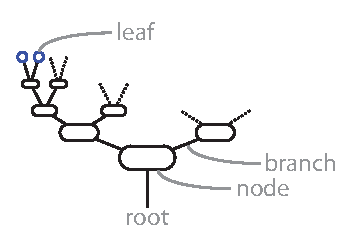
\includegraphics[width=.3\textwidth]{img/kdtree_naming}
	\caption[Naming in a tree structure]{Naming in a tree structure. The root contains the total memory, a leaf contains a single sample.}
	\label{fig:LLR-kdtree_naming}
\end{figure}

\paragraph{Splitting criterion}
The splitting criterion consists of two parts: the splitting-dimension and the splitting-value. The dimension is chosen based on the current level in the tree. In this way, the splitting-value cycles through all dimensions. The choice of the splitting-value is based on the values of the points (in the splitting-dimension) in the considered subset. We choose the median value. \figref{fig:LLR-kdtree_build} shows how a $k$d-tree is built, based on a data set of 16 samples.

Using the median value to split along a dimension leads to a balanced tree. In a perfectly balanced tree, all nodes have an equal number of 'left' and 'right' branches. A balanced tree is in general preferable, as an unbalanced tree could in theory lead to sub-optimal performance when searching for nearest neighbors. If the distribution of the data is not uniform over the state-space, a different splitting criterion might be preferable in order to prevent bad performance in the nearest neighbor search. 

\begin{figure}[htbp]
	\centering
		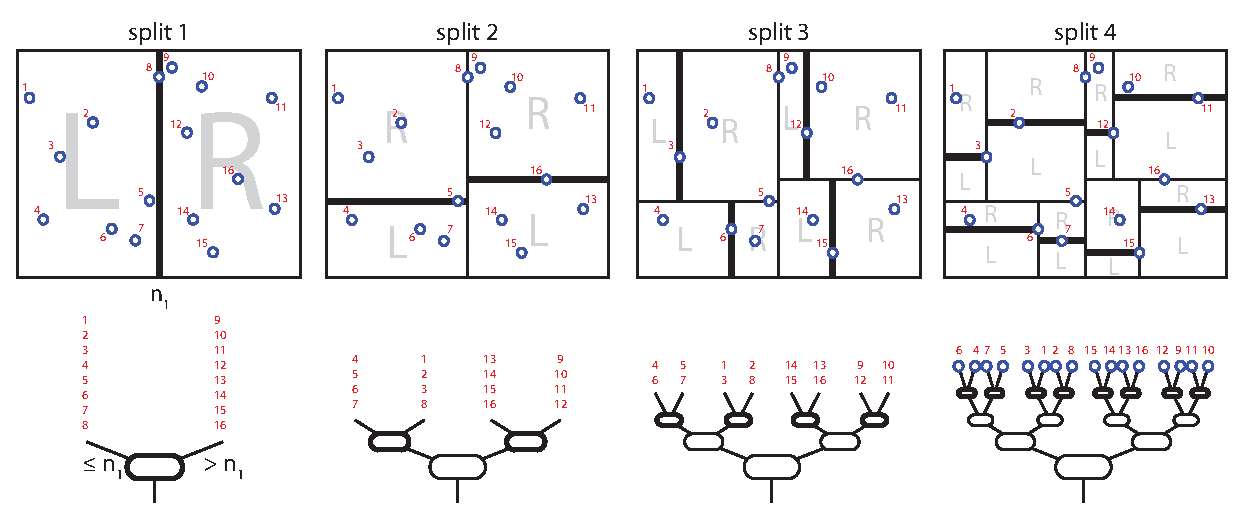
\includegraphics[width=\textwidth]{img/kdtree_buildv2}
	\caption[Construction of a $k$d-tree]{Creating a $k$d-tree structure to represent a set of 16 data samples in a two-dimensional space. 'L' indicates the points 'left' of a node, 'R' indicates the points 'right' of a node.}
	\label{fig:LLR-kdtree_build}
\end{figure}

\paragraph{Adding and removing samples}
Although building a new tree leads to a perfectly balanced tree, it takes considerable time for a large number of samples. This is caused by the fact that choosing the splitting values, requires sorting of all samples which is a slow process. For a set of $N$ samples of dimensionality $k$, constructing a tree is of complexity $O(kN\log{N})$ \cite{Berg:00}. Fortunately, re-building the entire tree is not always needed. Using the existing tree structure, new samples can be added to the tree. Adding samples to an existing tree is straightforward. Starting from the root of the tree, the tree is traversed. At every node, the choice 'left' or 'right' is based on the splitting criterion and the value of the to-be-added sample. In this way, the new sample ends up in a certain leaf. Because we only allow for one sample to be stored in a leaf, this leaf has to be converted into a new node that leads to two leafs: one containing the existing sample and one containing the to-be-added sample (see \figref{fig:LLR-kdtree_addsample}).

Continually adding new samples to an existing tree can cause the tree to become unbalanced. Especially when the number of added samples is relatively large compared to the original tree size. An unbalanced tree could lead to performance issues in the nearest neighbors search. A solution to this problem is to re-build the entire tree whenever the tree appears to become unbalanced. The approach in our experiments was to re-build the tree when the number of samples was less than 1000 and add new samples to the existing tree thereafter. This value was chosen because re-building a tree for 1000 samples was still relatively fast. Re-building a tree for more samples took too long to be convenient. With this approach, loss of performance due to an unbalanced $k$d-tree was never an issue.

Removing samples from an existing tree is simply the reverse of adding a sample. The to-be-deleted sample is removed and the node that led to that sample is converted into a leaf that contains the remaining sample. With the possibility of adding and removing samples, all tools are available to include memory management using a $k$d-tree to represent the data.

\begin{figure}[htbp]
	\centering
		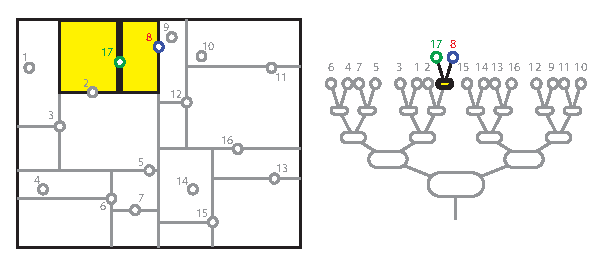
\includegraphics[width=.7\textwidth]{img/kdtree_addsample_treev2}
	\caption[Addition of a single sample to a $k$d-tree]{Adding a new sample to the existing $k$d-tree constructed in Figure \ref{fig:LLR-kdtree_build}. Sample 17 is added by creating a new node at the position of sample 8.}
	\label{fig:LLR-kdtree_addsample}
\end{figure}


\subsubsection{Nearest neighbors search using a $k$d-tree}
Our reason to store all data in a $k$d-tree is to speed up the nearest neighbors search. We will describe the search algorithm for finding a single nearest nearest neighbor, according to \cite{Friedman:77}. For this method it is assumed that the distance measure $D$ is monotonically increasing, which is true for all vector norms:
\begin{equation}\label{eqn:LLR-monotonicity}
%	D(\mathbf{x}_q,\mathbf{x}_1) \geq D(\mathbf{x}_q,\mathbf{x}_2) \textrm{, \quad    if } \mathbf{x}_1 > \mathbf{x}_2
%	D_i(\mathbf{x}_q,\mathbf{y}_i) \geq D_i(\mathbf{x}_q,\mathbf{z}_i) \textrm{, \quad    if } \mathbf{y}_i > \mathbf{z}_i
	D_i(x_{q,i},y_i) \geq D_i(x_{q,i},z_i) \textrm{, \quad    if } y_i > z_i
\end{equation}
With $i = 1, 2, ..., k$. $D_i$ is the distance measure for the $i$th dimension. 

We will describe the search for the nearest neighbor to a query point in a 2-dimensional space (\figref{fig:LLR-kdtree_NNsearch}). The search starts with moving down the tree to determine the leaf that would contain the query point. This is the same procedure as when a new sample was added to an existing tree. The point in the leaf is stored as 'current best'. The real nearest neighbor should be at least as close to the query point as this first leaf point. Therefore, a sphere with a radius equal to the distance to the current best is created around the query point. Using the values of the splitting criteria, the nodes that intersect with this sphere are identified. These nodes could possibly contain points that are closer than the current best and are therefore inspected. If a closer point is found, this is stored as current best. With this approach, large parts of the tree do not have to be visited. This approach is also valid in higher dimensions. For a more elaborate description of the search algorithm, see e.g. \cite{Moore:91}, \cite{Friedman:77}.

A $K$ nearest neighbors search is carried out in the same way. The only difference is that a list of $K$ current best points is stored, instead of a single best point. A new point is added to this list when it is closer that the $K$ nearest point. 

\begin{figure}[htbp]
	\centering
		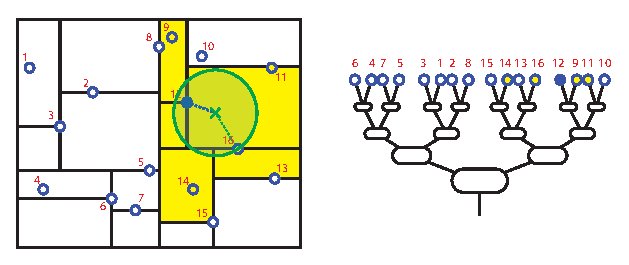
\includegraphics[width=.7\textwidth]{img/kdtree_NNsearch_treev2}
	\caption[Nearest neighbor search using a $k$d-tree]{Nearest neighbor search using a $k$d-tree structure. The green cross represents the query point. The first neighbor found is sample 16. All nodes that intersect with the green circle are then visited and eventually sample 12 is identified as the nearest neighbor. Using the $k$d-tree, the distance to the query point of only five samples (9, 11, 12, 14, 16) out of a total of sixteen samples had to be calculated.}
	\label{fig:LLR-kdtree_NNsearch}
\end{figure}


\paragraph{Performance}
The reason for using a $k$d-tree to store memory samples is to reduce the computational effort in the nearest neighbors search. Theoretically, the nearest neighbor search using a tree has complexity $O(\log(N))$ \cite{Friedman:77}, excluding the time needed to build the tree. So for large data sets, this method is preferred over a naive search, which has complexity $O(N)$.

%We empirically compared the $k$d-tree search with the standard naive approach for varying number of data points (Figure \ref{fig:LLR-kdtree_NNsearch_comp_effort}.
%\\
%\textcolor{red}{to be added: RESULTS: compare naive with kd-tree}
%
%\begin{figure}[htbp]
%	\centering
%		\includegraphics[height=200pt]{img/kdtree_NNsearch_comp_effort}
%		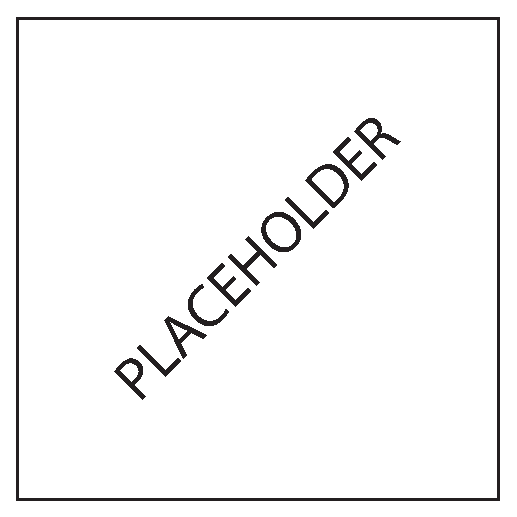
\includegraphics[height=200pt]{img/Placeholder}
%	\caption[Computation time needed for a nearest neighbors search using a $k$d-tree and the naive approach]{Calculation time needed for a nearest neighbors search ($K=50$) on a set of samples. The naive approach and the $k$d-tree implementation are compared.}
%	\label{fig:LLR-kdtree_NNsearch_comp_effort}
%\end{figure}

The nearest neighbors search discussed here, always returns the exact $K$ closest neighbors. A way to reduce computation time even more, is to use an approximate search algorithm. Such an algorithm also returns $K$ neighbors, but not necessarily the closest.  For on-line applications with a large number of memory samples a fast search might be more important than an exact search. The approximate nearest neighbors search might be useful to reduce computation time in such cases. However, approximate nearest neighbor methods are outside the scope of this research.
%Such algorithms are for example \textcolor{red}{****} and can be found in \textcolor{red}{[REF]}.

\subsubsection{Limitations}
Although using a tree structure to find the set of nearest neighbors significantly increases the searching speed, some limitations do exist. We will discuss two problems.

\paragraph{Wrapping angles} Many systems with rotational degrees of freedom, have rotational symmetry. Adding a full $2\pi$ rotation to a variable does not change the physical state of the system. Therefore, those state-variables are usually wrapped on a $2\pi$ domain ($[0,2\pi)$ for instance). The nearest neighbors search should be able to deal with this wrapped domain when calculating distances. For instance, the points $x_1=0$ and $x_2=2\pi$ should have a distance of $0$, instead of $2\pi$.

In the naive approach dealing with wrapping can be done by, for instance, translating all data points such that the query point is in the center of the wrapped domain or by introducing an alternative distance measure that incorporates wrapping. These approaches are not possible when a tree structure is used. Manipulating data points would require re-building of the entire tree, which is unwanted for large data sets. An alternative distance measure would violate the monotonicity requirement \eqnref{eqn:LLR-monotonicity}, which would cause the nearest neighbors search to fail. To our knowledge an implementation of $k$d-trees that deals with wrapped domains does not exist. Development of such a 'circular' $k$d-tree could be an interesting and useful future research topic. 

In this work we will simply ignore the wrapping problem. For data sets with a sufficiently high sample density near the edges of the wrapped domain, this should not lead to problems.

\paragraph{Building time} The reason we are using a $k$d-tree, is for speeding-up the $K$ nearest neighbors search. As we have shown, this process is significantly faster using a tree than using a sorting algorithm. However, the time needed for building the tree is still large. This is due to the fact that selecting the median values in a certain dimension to use as splitting values still involves sorting all data points. If one would continuously re-build the entire tree, this would be a major issue. In our experiments, we have chosen the following approach to deal with this problem: We build an initial tree from a large number of data point and add new points to the existing tree. The possible loss of performance was not observed, possibly because the initial tree was built using a sufficiently large number of data points.







\subsection{Linear regression}\label{sec:LLR-linear regression}
Once the set of $K$ nearest neighbors is determined, the second step of the \ac{LLR} method is fitting a linear model to the obtained set of data. Linear regression is a well known technique and has been thoroughly analyzed in the literature (see for example \cite{Rencher:08}). In this section, we will select useful results from the literature that will be used in this work. First, we will introduce the linear regression model. Thereafter we will describe prediction intervals and outlier detection as possible techniques to assess and increase the quality of the estimates.




\subsubsection{Estimating a linear model}\label{sec:LLR-linear model}
We assume that the state-transition model can be represented locally by a linear model with the following structure:
$$
	\left(\begin{array}{c} y_1 \\ y_2 \\ \vdots \\ y_{d_y} \end{array}\right) = 
	\left(\begin{array}{c} x_1 \\ x_2 \\ \vdots \\ x_{d_x} \end{array}\right)^T 
	\left(\begin{array}{cccc} 
		\beta_{1,1} 	& \beta_{1,2} 	& \hdots 	& \beta_{1,d_y} 	\\
		\beta_{2,1} 	& \beta_{2,2} 	& \hdots 	& \beta_{2,d_y} 	\\
		\vdots 				& \vdots 				& \ddots 	& \vdots 				\\
		\beta_{d_x,1} & \beta_{d_x,2} & \hdots 	& \beta_{d_x,d_y}
	\end{array}\right) + 
	\left(\begin{array}{c} \epsilon_1 \\ \epsilon_2 \\ \vdots \\ \epsilon_{d_y} \end{array}\right)
$$
Or in vector notation:
\begin{equation}
	\mathbf{y} = \mathbf{x}^T\bm{\beta} + \bm{\epsilon}
	\label{eqn:LLR-linear system}
\end{equation}
Where \lsymb{$\mathbf{y}$}{Output vector} is a $d_y \times 1$ output vector, \lsymb{$\mathbf{x}$}{Input vector} is a $d_x \times 1$ input vector\footnote{We will use $\mathbf{x}$ and $\mathbf{y}$ to represent input and output in this section. Note that in a real application $\mathbf{x}$ would contain states $x_t$ and actions $u_t$ and $\mathbf{y}$ would contain next states $x_{t+1}$, as explained in \ref{sec:LLR-memory-based modeling}}, \gsymb{$\bm{\beta}$}{Regression variable} is a $d_x \times d_y$ matrix. The regression variable $\bm{\beta}$ represents the local state-transition model and consists of $d_x d_y$ regression coefficients. The $d_y \times 1$ vector \gsymb{$\bm{\epsilon}$}{Noise vector} is the noise vector. By definition, the error vector has the following properties:
\begin{enumerate}
	\item $E\left[\bm{\epsilon}\right]=\bm{0}$, hence $E\left[ \mathbf{y} \right] = E\left[ \mathbf{x}^T\bm{\beta} \right]$
	\item $\textrm{cov}(\bm{\epsilon})=\sigma^2\bm{I}$, hence $\textrm{cov}(\mathbf{y})=\sigma^2\bm{I}$
\end{enumerate}
Where $E[\cdot]$ denotes the expected value. The first property assumes that the error is zero mean and that the samples represent a linear function. The second property assumes that the individual noise terms are independent and their variance equals \gsymb{$\sigma^2$}{Noise variance}. 

The linear model is estimated based on $K$ observations (which result from the nearest neighbors search). These can be written in matrix form as:
$$
	\left( \begin{array}{c} \mathbf{y}_1^T \\ \mathbf{y}_2^T \\ \vdots \\ \mathbf{y}_K^T \end{array} \right) = 
	\left( \begin{array}{c} \mathbf{x}_1^T \\ \mathbf{x}_2^T \\ \vdots \\ \mathbf{x}_K^T \end{array} \right)
	\bm{\beta} + \left( \begin{array}{c} \bm{\epsilon}_1^T \\ \bm{\epsilon}_2^T \\ \vdots \\ \bm{\epsilon}_K^T \end{array} \right)
$$
Or in short:
$$\label{eqn:LLR-linear model}
	\mathbf{Y} = \mathbf{X}\bm{\beta} + \bm{E}
$$
With \lsymb{$\mathbf{X}$}{Input matrix} the input matrix and \lsymb{$\mathbf{Y}$}{Output matrix} the output matrix. The regression variable $\bm{\beta}$ has $d_y d_x$ regression coefficients. In order to uniquely identify $\bm{\beta}$ from $K$ samples, it is required that $\textrm{rank}(X) \geq K$. This means that we require at least $K \geq d_x$ observations.
The \ac{LLR} model is estimated using the least squares approach. We try to minimize the sum of the squared errors:
$$ 
 \sum_{i=1}^{K}{ \hat{\mathbf{e}}_i^2} = \sum_{i=1}^{K}{\left( \mathbf{y}_i - \mathbf{\hat{y}}_i\right)^T\left( \mathbf{y}_i - \mathbf{\hat{y}}_i\right)}
$$
Where $\mathbf{\hat{y}}_i = \mathbf{x}_i^T\bm{\hat{\beta}}$ is the prediction of $\mathbf{y}_i$. We use $\hat{\cdot}$ to denote a predicted quantity. In matrix notation, the sum of squared errors is:
$$
	\hat{\bm{E}}^T\hat{\bm{E}} = \left(\bm{Y}-\bm{X}\hat{\bm{\beta}}\right)^T\left(\bm{Y}-\bm{X}\hat{\bm{\beta}}\right)
$$ 
Differentiating the squared error with respect to $\bm{\beta}$ and setting the result equal to zero, leads to the normal equations:
$$
	\bm{X}^T\bm{X}\hat{\bm{\beta}} = \bm{X}^T\mathbf{Y}
$$
Therefore, the least squares solution to \eqnref{eqn:LLR-linear model} is:
$$
	\bm{\hat{\beta}} = \left(\bm{X}^T\bm{X}\right)^{-1}\bm{X}^T\bm{Y}
$$
Note that in practice, calculating $\left(\bm{X}^T\bm{X}\right)^{-1}$ explicitly is wanted nor needed. Instead, the normal equations are solved using matrix manipulations (such as Gaussian elimination).

\subsubsection{Model accuracy}\label{sec:LLR-model accuracy}
\paragraph{Estimation error}\label{sec:LLR-estimation error} The obtained linear model is used to estimate a state-transition. Or, using input-output terminology, estimate the output for a given input query:
$$
	\mathbf{\hat{y}}_q = \mathbf{x}_q \bm{\hat{\beta}}
$$
We would like to have a measure to assess the accuracy of the predicted output. In the field of system identification, the quality of a model is usually assessed by comparing the estimated (model) output to the measured (real) output. For a single prediction, we can simply use the residual vector \lsymb{$\mathbf{e}$}{Residual vector}:
$$
	\mathbf{e} = \left| \mathbf{\hat{y}}_q - \mathbf{y}_q \right| 
$$ 
If we want to assess the quality of a set of estimates, we can use the \ac{RMSE} of a set of $M$ predictions:
$$
%	\textrm{RMSE} = \sqrt{ \frac{1}{M} \left( \hat{y}(t)-y(t) \right)^T \left( \hat{y}(t)-y(t) \right) }
	\textrm{RMSE} = \sqrt{ \frac{1}{M} \sum_{t=1}^{M}{\left(\mathbf{\hat{y}}(t) - \mathbf{y}(t) \right)^T \left(\mathbf{\hat{y}}(t) - \mathbf{y}(t) \right) }}
$$
A measure comparing the estimated output to the measured output, will be referred to as the \ac{RMS} \emph{estimation error}. 

However, such methods can only be used if the real output is available. In our case, we want to apply the \ac{LLR} model in a \ac{RL} setting. We will not always have the real output available to compare the estimated output to. So we would like to have an accuracy measure that is based on the data used in the linear regression and not on a measured output. Such a measure will be called the \emph{prediction accuracy}. The expressions for the prediction accuracy will be discussed next.

\paragraph{Prediction accuracy}\label{sec:LLR-prediction interval}
The accuracy of a predicted output will be given as a confidence interval around the estimated output. It can be shown (see Appendix \ref{sec:app-statistics_PredInt}) that the t-statistic:
$$
	 t = \frac{ \mathbf{y}_q - \mathbf{\hat{y}}_q }{ \sigma \sqrt{1 + \mathbf{x}_q^T \left( \bm{X}^T \mathbf{X} \right)^{-1} \mathbf{x}_q} }
$$
is zero mean and has a $t(K-d_x)$ distribution. The noise variance $\sigma^2$ can be estimated by $s^2$ (\eqnref{eqn:app-statistics_s}). Using the probability density function of the $t$-distribution, we can obtain a $100(1-\alpha)\%$ confidence interval for the estimate $\mathbf{\hat{y}}_q$:
$$
	\mathbf{y}_q = \mathbf{\hat{y}}_q \pm t_{\alpha/2,K-d_x} s \sqrt{1 + \mathbf{x}_q^T \left( \bm{X}^T \bm{X} \right)^{-1} \mathbf{x}_q}
$$
These formulas can be used as a quality measure of the estimated outputs, based solely on information that can be obtained from the dataset. This measure will be called a prediction interval $I$ and we can write:
$$
	\mathbf{y}_q = \mathbf{\hat{y}}_q \pm I
$$
Throughout this report we have used $\alpha=0.05$, which gives a 95\% confidence interval around a predicted output.

It is important to note that these equations are statistical measures that are derived, based on assumptions on the data-generating function. The most important assumption is that the generating function is linear. In our experiments, we assume that the functions we are estimating are locally linear and that the nearest neighbors represent this local linearity. Therefore we argue that the statistical results are valid. However, the nearest neighbors might not represent a linear function when the target function is highly nonlinear or the sample density is low. In these cases the samples used in the linear regression do not represent a linear system \eqnref{eqn:LLR-linear model} and the equations are not valid. In fact, the prediction interval may severely underestimate the possible prediction error in the output. Therefore, this measure has to be used with care. The same holds for the equations derived for outlier detection in the next section.

\subsubsection{Outlier detection}\label{sec:LLR-outlierdetection}
A set of data, obtained from measurements on a real system, typically contains a certain amount of faulty data. These faulty samples can be the result of disturbances or measurement errors. \ac{LLR} is a method that is sensible to noise because no global structure is imposed on the data. Since faulty samples could lead to an inaccurate model, it is useful to be able to identify these samples and optionally ignore them in the estimation process. Samples that are far away from the linear model that is fitted to the data are called outliers.

We again use a measure from the field of statistics to determine the presence of outliers. We use the \ac{PRESS} statistic:
$$
	\textrm{PRESS} = \sum_{i=1}^{K}{ \left( \frac{\mathbf{y}_i - \mathbf{x}_i^T\bm{\beta}}{s\sqrt{1-\mathbf{x}_i^T \left( \bm{X}^T \bm{X} \right)^{-1} \mathbf{x}_i}} \right)^2 }
$$
The individual contribution of each data point to \ac{PRESS} is:
$$
	e_i = \frac{\mathbf{y}_i - \mathbf{x}_i^T\bm{\beta}}{s\sqrt{1-\mathbf{x}_i^T \left( \bm{X}^T \bm{X} \right)^{-1} \mathbf{x}_i}}
$$
This measure has a normal distribution with zero mean and unit variance. If the residual of a point is larger than a certain threshold, the point is called an outlier. We use 1.96, which is the value that cuts off the 5\% area of a normal distribution. 


\subsection{Computational complexity}
An advantage of memory-based modeling, is that at every moment the full dataset is available to perform various analysis and optimization calculations. In this section we have only discussed prediction intervals and outlier detection but many more useful calculations could be thought of. In simulation, the addition of extra calculations is virtually unlimited. In a real-time system however, the amount of time available to make calculations is limited and is dictated by the sampling time. So, all calculations must be performed in the given sampling interval, which means that the number of calculations that can be performed is limited. 

In this work, \ac{LLR} is used as a model building technique in a \ac{RL} setting. We are using \ac{LLR} as a way to increase learning speed by generating state-transitions. We are not necessarily interested in estimating a very accurate model. In Chapter \ref{chap:Prioritized Sweeping} we will show an example in which it is more useful to estimate many inaccurate state-transitions than to estimate less very accurate state-transitions. So whether or not the statistical methods are useful in practice might depend on the specific application.






\section{Experimental results}\label{sec:LLR-results}
In Section \ref{sec:LLR-local linear regression} we introduced \ac{LLR} as a modeling method and introduced statistics that can be used to assess and improve the estimation accuracy of the model. In this section we will apply \ac{LLR} in three settings. First we will estimate a 1-dimensional nonlinear function. Using this example, we can easily investigate and visualize the results of the \ac{LLR} method. Thereafter we will use \ac{LLR} as a method to model state-transitions on two different setups. The first setup is a simulation of a two-link manipulator. This system has got four state-variables and two inputs. The second setup is a humanoid robot setup. This is a complex setup that has 18 state-variables and 6 inputs.

\subsection{1D nonlinear function}\label{sec:LLR-results_nonlinear}
Before using \ac{LLR} to model state-transitions of a real system, we will investigate how the results of Section \ref{sec:LLR-model accuracy} can be used. To easily visualize the results of this section, we use the following 1-dimensional, nonlinear test function: 
\begin{equation}\label{eqn:LLR-nonlinear test function}
		y = x- \sin^3(2\pi x^3) \cos(2\pi x^3) \exp(x^4)
\end{equation}
on the domain $x \in [0, 1]$. This nonlinear test function is useful, because it contains both high-frequency and low-frequency components. We estimate a model $\hat{\bm{\beta}}$ that estimates the output \lsymb{$\hat{y}$}{Estimated output} using $K$ inputs samples around \lsymb{$x_q$}{Query input}:
$$
	\hat{y} = \begin{bmatrix} x_q \\ 1 \end{bmatrix}^T \hat{\bm{\beta}}
$$
We add 1 to the input vector to prevent that the linear model has to cross the origin. A dataset of $N = 100$ randomly distributed samples was generated and a white noise signal with $\sigma^2 = 0.01$ was added to the output (see \figref{fig:LLR-nonlinfunction_dataset}). Using this nonlinear function we would like to answer the following questions regarding the \ac{LLR} method:
\begin{enumerate}
	\item Can the prediction interval be used to assess the quality of the estimate?
	\item Is outlier detection useful to increase the estimation accuracy?
	\item Can we locally tune the number of nearest neighbors to increase the estimation quality?
\end{enumerate}


\subsubsection{Prediction intervals}
\figref{fig:LLR-nonlinfunction_estimate} shows the \ac{LLR} estimate (using $K=4$) of the nonlinear test function with prediction intervals that indicate the quality of the estimate. The target function was estimated at $x_q = 1, 0.01, ..., 1$. The estimation is reasonably good in low-frequency areas (small values of $x$) but in high frequency areas (large values of $x$), the estimate is less accurate. The reason is that the sample density is too low to represent the fast dynamics of the target function accurately. This leads to a set of $K$ samples that do not represent a linear function around $x_q$. This is represented by the prediction intervals that are large for these areas, but much smaller for the more accurate estimates. 

\figref{fig:LLR-nonlinfunction_predint} shows the size of the prediction interval compared to the estimation error $\left| \hat{y} - y \right|$. We can clearly see that the prediction interval is no actual accuracy measure: the shape of the interval does not exactly match the shape of the error. However, the prediction interval is significantly larger for large values of $x$ and smaller for small values of $x$. This effect follows from the definition of the prediction interval. It should be used as a measure of linearity of samples instead of accuracy of prediction. However, if the samples are highly nonlinear, we can expect the estimated output to be inaccurate (or at least uncertain). So we argue that this measure can still be used to assess the quality of the prediction.

\begin{figure}[htbp]
	\centering
	\subfigure[Dataset obtained from the nonlinear function]{
	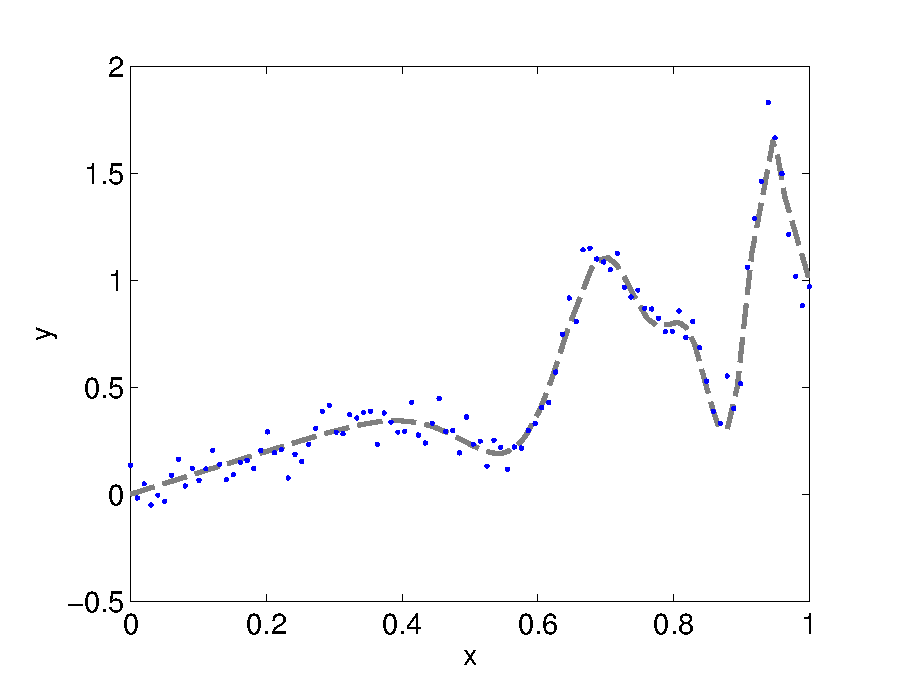
\includegraphics[width=.45\textwidth]{Figures/LLR-nonlinfunction}
	\label{fig:LLR-nonlinfunction_dataset}
	}\\
	\subfigure[\ac{LLR} estimate of the nonlinear function]{
	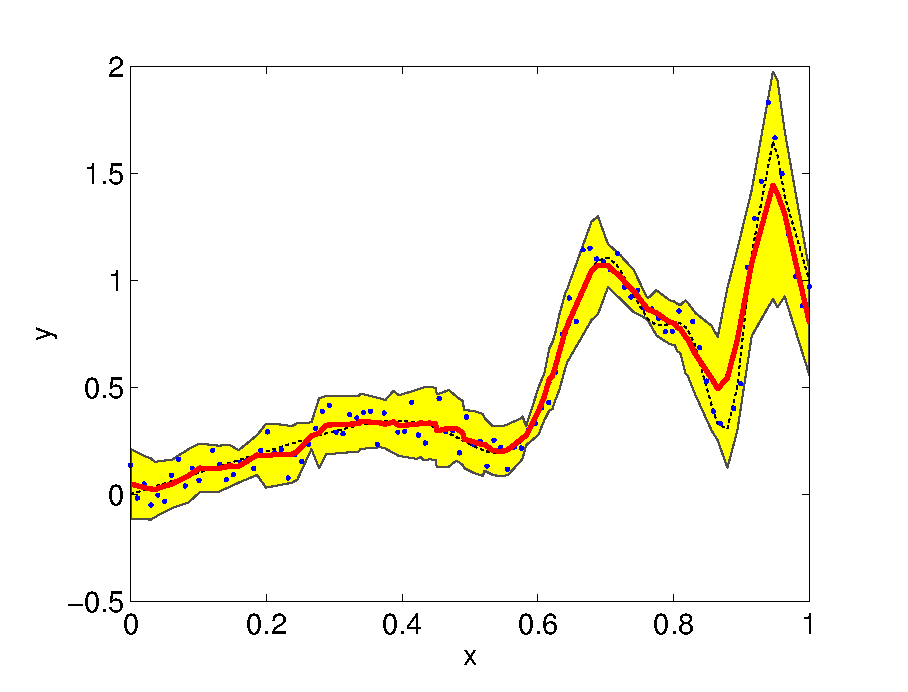
\includegraphics[width=.45\textwidth]{Figures/LLR-nonlinfunction_globalk}
	\label{fig:LLR-nonlinfunction_estimate}
	}\\
	\subfigure[Prediction interval compared to the estimation error]{
	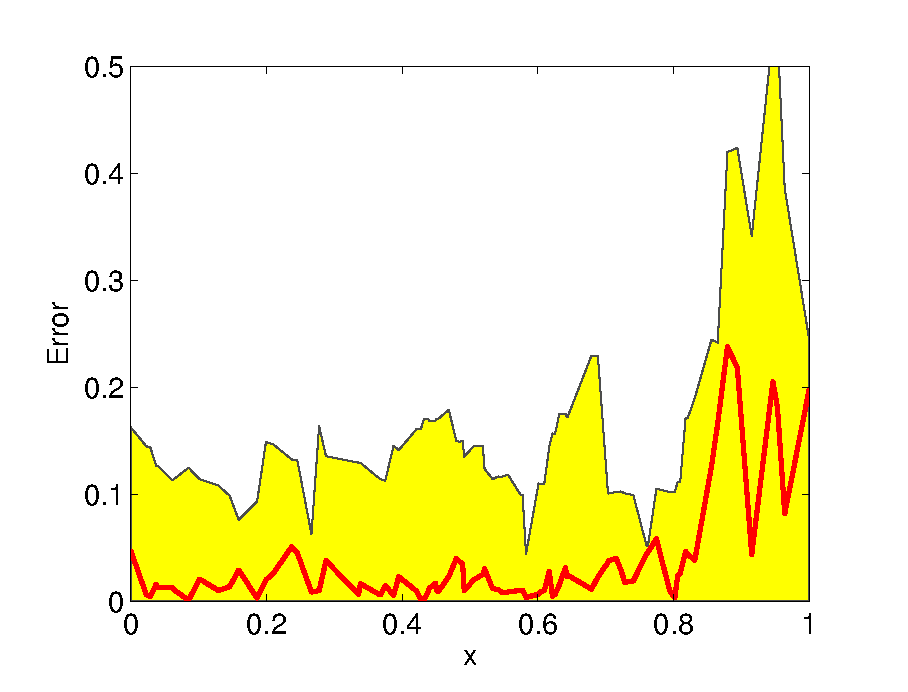
\includegraphics[width=.45\textwidth]{Figures/LLR-nonlinfunction_predint}
	\label{fig:LLR-nonlinfunction_predint}
	}
	\caption[\acs{LLR} estimate of a nonlinear function]{\ac{LLR} estimate of a 1-dimensional nonlinear function. \subref{fig:LLR-nonlinfunction_dataset} shows 100 noisy samples (dots) obtained from the nonlinear function \eqnref{eqn:LLR-nonlinear test function} (dashed line). \subref{fig:LLR-nonlinfunction_estimate} shows the resulting \ac{LLR} estimate (solid line) of the nonlinear function (dashed line) using $K=4$ with prediction intervals (shaded area) estimated at 100 query points. \subref{fig:LLR-nonlinfunction_predint} shows the estimation error $\left| \hat{y} - y \right|$ (solid red line) compared to the size of the prediction interval (shaded area).}
	\label{fig:LLR-nonlinfunction}
\end{figure}


\subsubsection{Outlier detection}
To test if we can use the methods of Section \ref{sec:LLR-outlierdetection} to identify faulty data, we replaced four samples of the original dataset of \figref{fig:LLR-nonlinfunction_dataset} by faulty data. \figref{fig:LLR-outlierdetection_without} shows the result that the outliers have on the estimation of the target function. We notice that the prediction is severely effected by the presence of the outliers. This is in turn represented by the prediction intervals, which are very large for the estimates that use the outliers.
 
\figref{fig:LLR-outlierdetection_with} shows the result when outlier detection is used. The data points that are identified as outliers are indicated by circles. When outliers were detected the \ac{LLR} estimate was computed again, neglecting the outlier(s). The added outliers are identified correctly. The result is clearly visible by the prediction intervals that are much smaller when the outliers are neglected. Also the \ac{LLR} estimate $\hat{y}$ becomes better when the outliers are neglected.

We notice that not only the added outliers are detected, but also the sample at $x = 0.72$ is identified as outlier. This is caused by the fact that the noisy data samples around this point are almost linear. This causes the identified linear model to match all points very accurately except for one point, which is therefore identified as outlier.

In our approach, we simply neglected outliers that were detected. An other approach could be to remove detected outliers from the memory. We do not opt for this approach because a sample that appears to be an outlier for a certain query point at one moment in time, could prove to be an usable sample for a different query point or at a later stage when more samples have been added to the memory. In general, we do not encourage removing or changing memory data. 
 
\begin{figure}[htbp]
	\centering
	\subfigure[Without outlier detection]{
	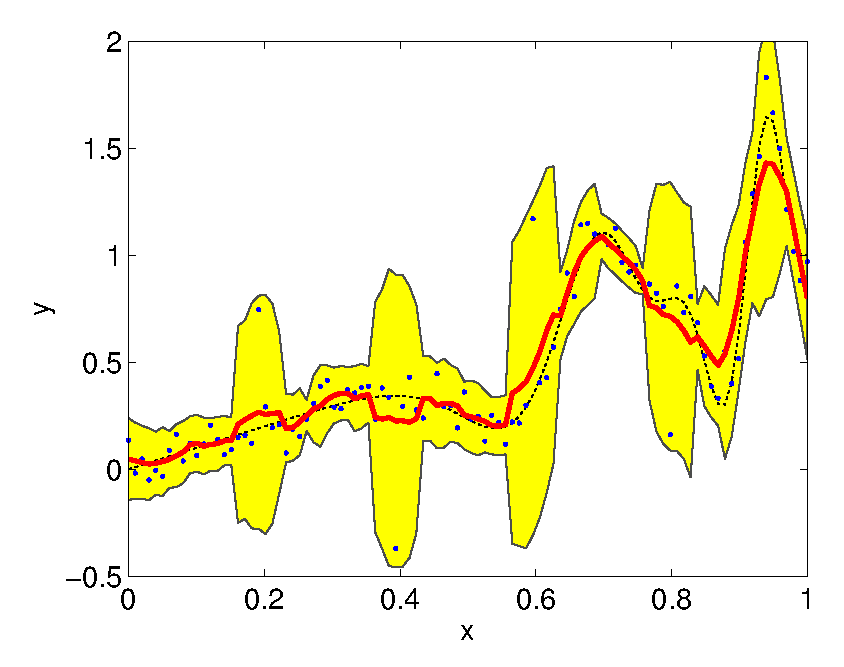
\includegraphics[width=.45\textwidth]{Figures/LLR-outlierdetection_without}
	\label{fig:LLR-outlierdetection_without}
	} 
	\subfigure[With outlier detection]{
	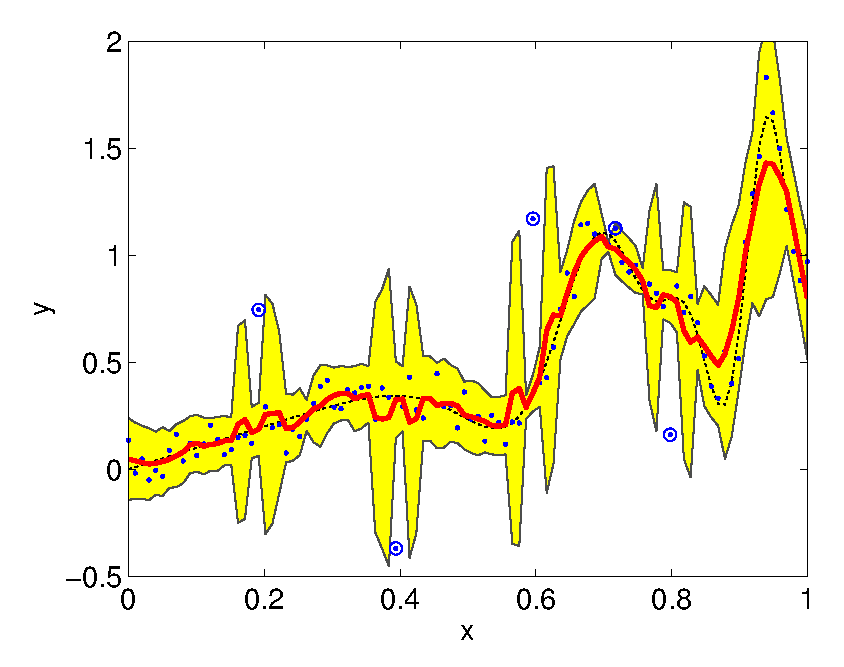
\includegraphics[width=.45\textwidth]{Figures/LLR-outlierdetection_with}
	\label{fig:LLR-outlierdetection_with}
	}
	\caption[Outlier detection in \ac{LLR}]{\ac{LLR} estimate with $K=4$ (solid line) of a nonlinear function (dashed line) with outliers added at $x=0.2,0.4,0.6,0.8$. \subref{fig:LLR-outlierdetection_without} shows the resulting estimate when the outliers are used in the estimation. \subref{fig:LLR-outlierdetection_with} shows the result when outliers are detected and neglected in the estimation. Data points that are identified as outliers are indicated by circles.}
	\label{fig:LLR-outlierdetection}
\end{figure}



\subsubsection{Optimizing the number of neighbors}\label{sec:LLR-optimal number of neighbors}
One of the attractive properties of \ac{LLR} is that the method has only got one parameter to tune: the number of nearest neighbors $K$ used in estimating the linear model. The optimal number of neighbors leads to the best estimation of the output (i.e., the smallest estimation error). The optimal number can vary throughout the state-space and depends locally on a number of factors:
\begin{itemize}
	\item Linearity of the function (highly nonlinear, smaller $K$)
	\item Sample density (more samples, higher $K$)
	\item Amount of noise (more noise, higher $K$)
\end{itemize}
Because these factors can vary over the state-space, the optimal number of nearest neighbors can also vary over the state-space. \figref{fig:LLR-optimal_K_schematic} schematically shows the estimation error as a function of $K$ for three different target functions:
\begin{enumerate}
	\item Linear function with noise
	\item Nonlinear function without noise
	\item Nonlinear function with noise
\end{enumerate}
In the first case (\figref{fig:LLR-optimal_K_schematic_a}), the number of neighbors should be high as possible to cancel the effect of noise. In fact, for white noise and $K\rightarrow \infty$ the \ac{LLR} estimate $\hat{y}(x_q)$ is an unbiased estimator of $y(x_q)$.

In the second case (\figref{fig:LLR-optimal_K_schematic_b}), the optimal choice is to simply take the output of the nearest neighbor as the estimated output. Including more neighbors will introduce a bias, since the target function is locally nonlinear.

The third case is the most interesting since this situation will generally be encountered in practice. Starting from $K=1$, increasing the number of nearest neighbors will reduce the estimation error, because the effect of noise is reduced. Further increasing $K$, will increase the error as the nonlinearity results in a biased estimate. So an optimal value for $K$ exists for which the estimation error is smallest.

Determining the optimal value for $K$ can be problematic, since no analytical expression to determine the optimal value for $K$ exists. Furthermore, even if we have a measure for the estimation error for a certain value of $K$, we do not have a method to determine whether this error is due to noisy samples or due to local nonlinearity of the target function. In the first case $K$ has to be increased, while in the second case it has to be decreased. In the next paragraph we will describe how the prediction interval could be used to tune the number of nearest neighbors.

\begin{figure}[htbp]
\centering
\subfigure[Linear target function with noise]{
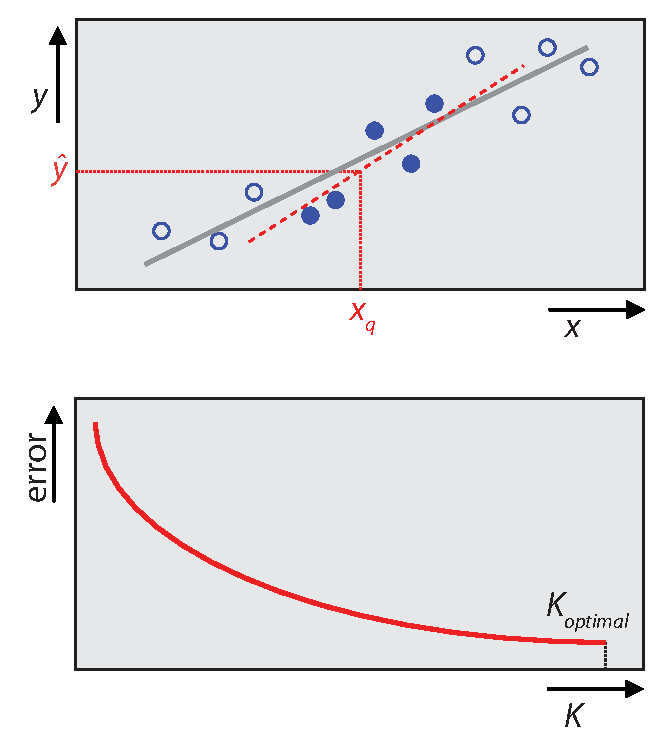
\includegraphics[width=.3\textwidth]{img/Koptimal_schematic_a}
\label{fig:LLR-optimal_K_schematic_a}
}
\subfigure[Nonlinear target function without noise]{
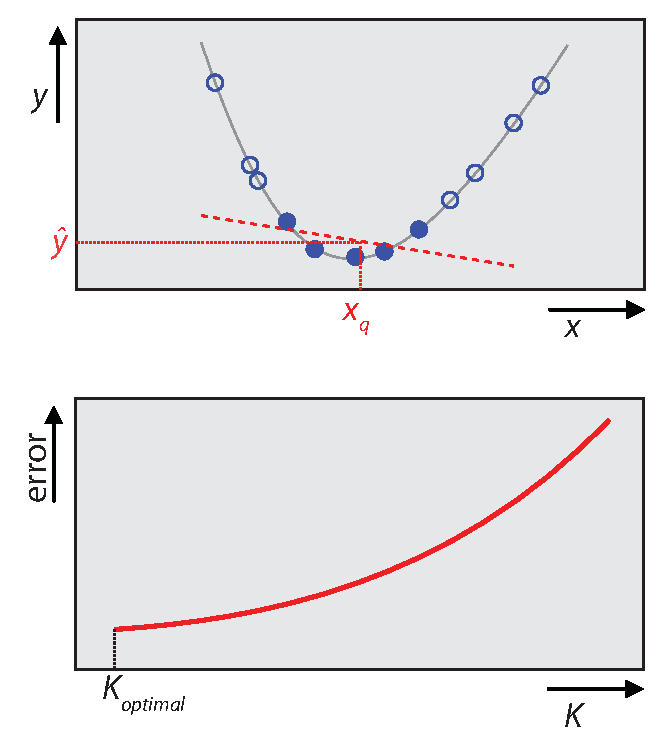
\includegraphics[width=.3\textwidth]{img/Koptimal_schematic_b}
\label{fig:LLR-optimal_K_schematic_b}
}
\subfigure[Nonlinear target function with noise]{
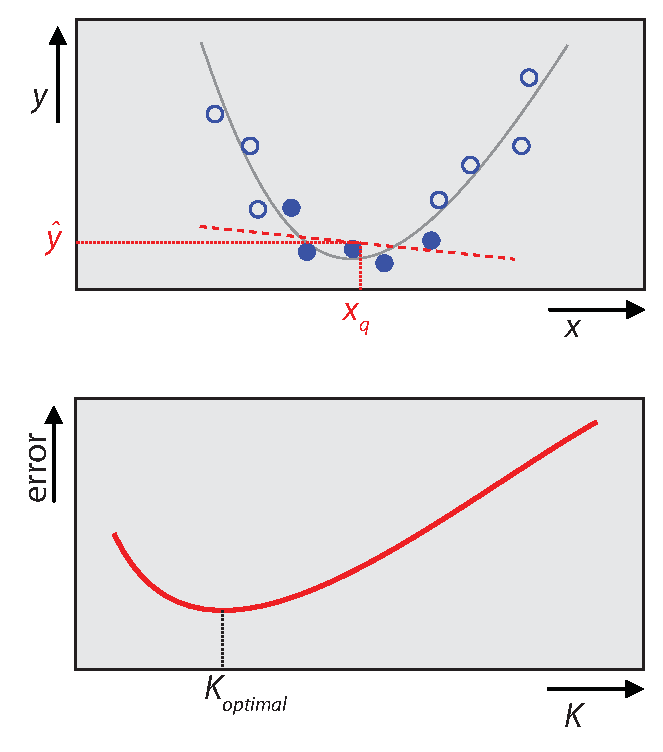
\includegraphics[width=.3\textwidth]{img/Koptimal_schematic_c}
\label{fig:LLR-optimal_K_schematic_c}
}
	\caption[Optimal number of neighbors for three different target functions]{Optimal number of neighbors for three different cases. \subref{fig:LLR-optimal_K_schematic_a} linear target function with added noise, \subref{fig:LLR-optimal_K_schematic_b} nonlinear target function without noise and \subref{fig:LLR-optimal_K_schematic_c} nonlinear target function with added noise. The top figures show a typical distribution of data points and the resulting linear regression. The bottom figures show schematically the absolute value of the estimation error of the real output and the estimated output as a function of the number of neighbors $K$.}
	\label{fig:LLR-optimal_K_schematic}
\end{figure}
	

\paragraph{Globally optimal $K$}
The general approach to tuning the value of $K$ is using the globally optimal value. A global optimum means a single fixed $K$ value that leads to the best estimation error on average. In practice, this means computing a model for several values of $K$ for a set of query points. The value that leads to the smallest total residual value will be chosen as globally optimal. This approach will typically lead to a model that is too general in fast dynamics regions and too noise sensitive in slow dynamics regions.

\figref{fig:LLR-K_varying} shows the RMS error of the estimation of the dataset of \figref{fig:LLR-nonlinfunction_dataset} for a range of different $K$ values. Since the target function is noisy and nonlinear, we expect the behavior as depicted in \figref{fig:LLR-optimal_K_schematic_c}. The expected behavior (first a decrease in error, then an increase) is indeed visible. Based on this figure, we select the globally optimal value $K=4$. 
%\begin{figure}[htbp]
%	\centering
%%		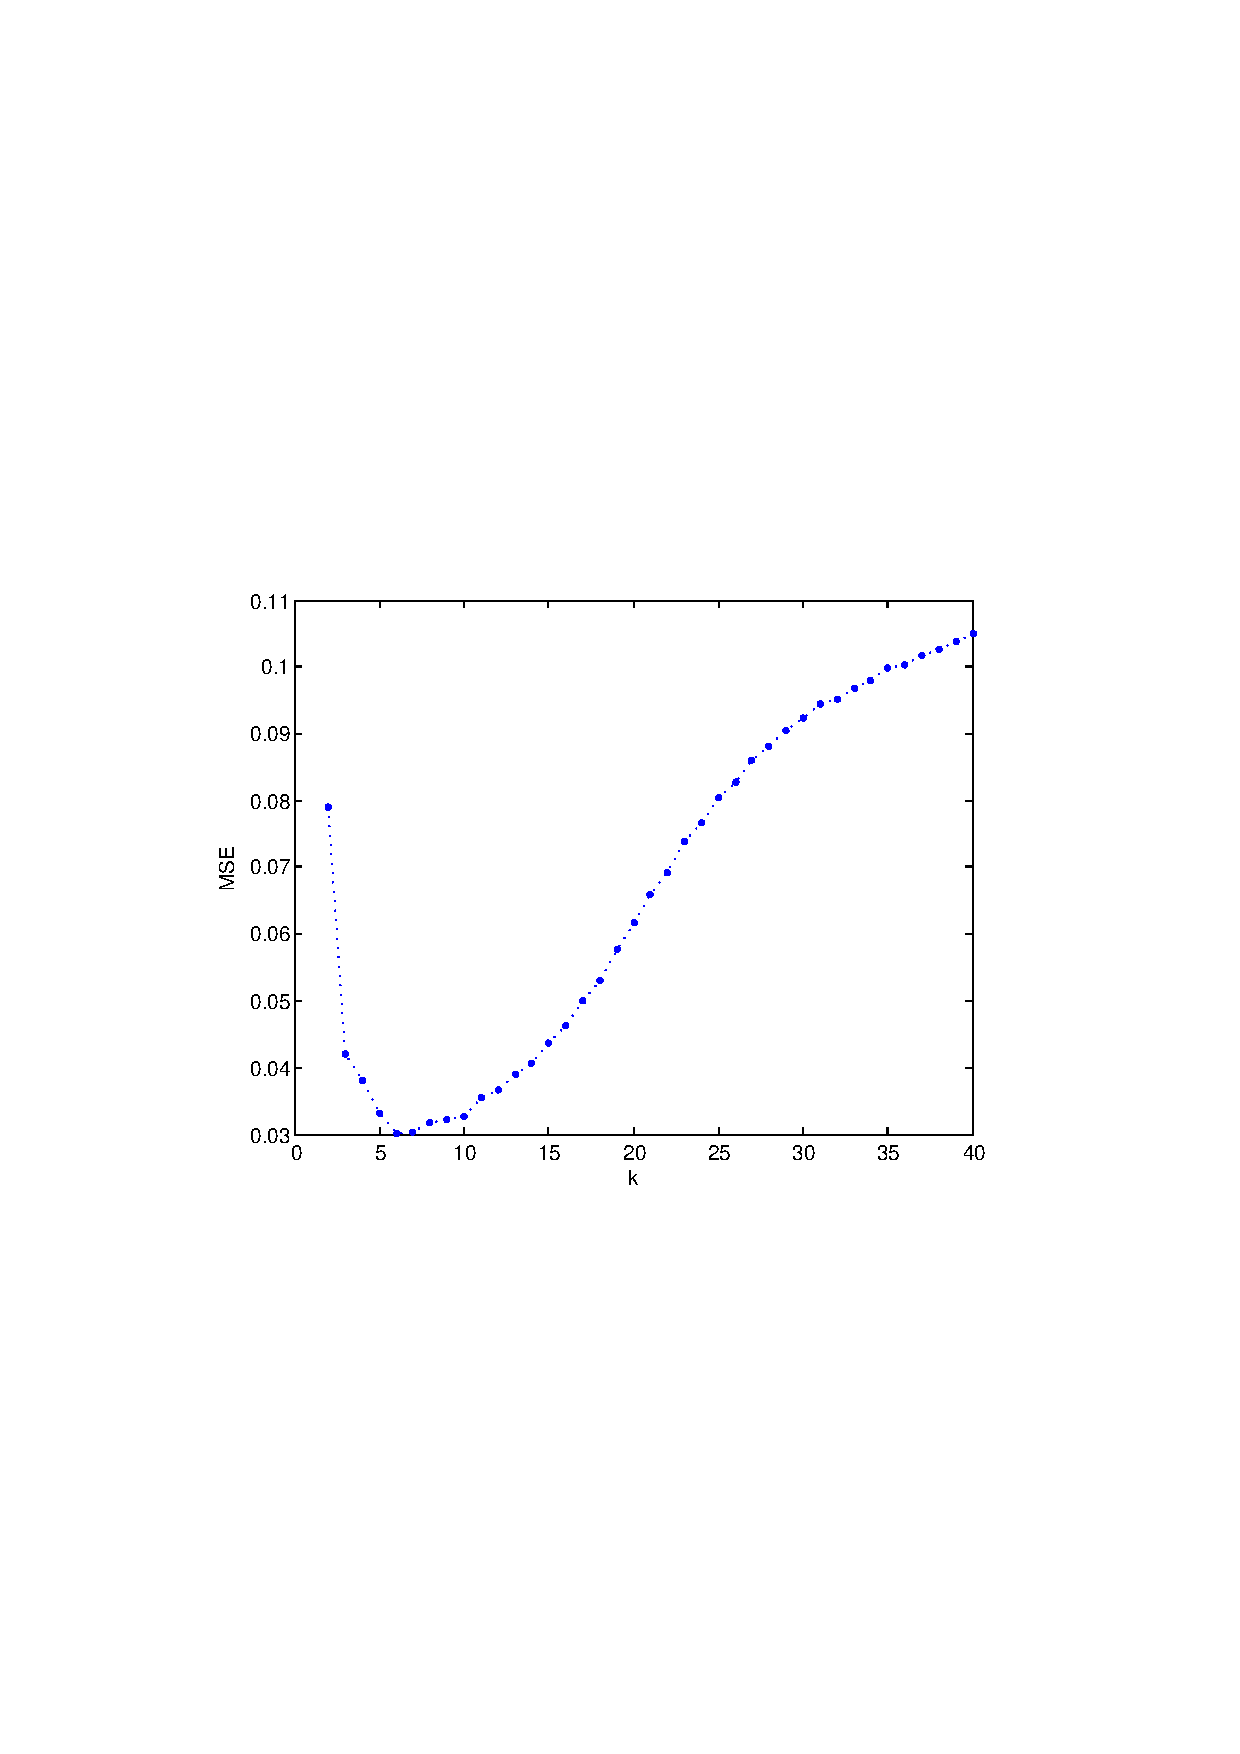
\includegraphics[width=.5\textwidth]{Figures/k_varying}
%		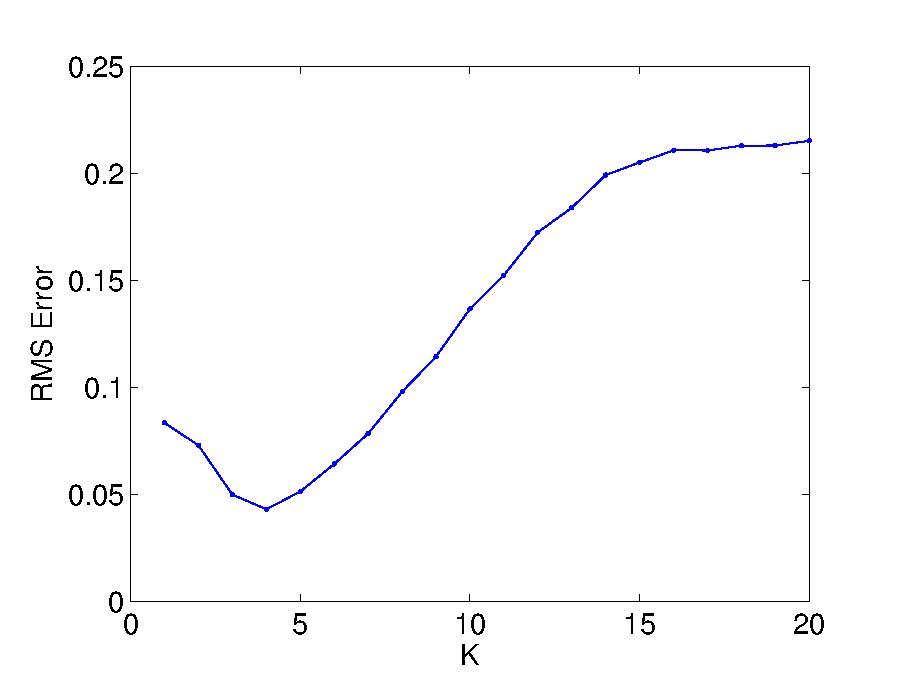
\includegraphics[width=.5\textwidth]{Figures/LLR-nonlinfunction_var_K}
%	\caption[Estimation error for a range of $K$ values]{RMS estimation error for a range of different $K$ values for the nonlinear target function.}
%	\label{fig:LLR-K_varying}
%\end{figure}

\begin{figure}[htbp]
	\centering
	\subfigure[Global optimum: $K=4$]{
	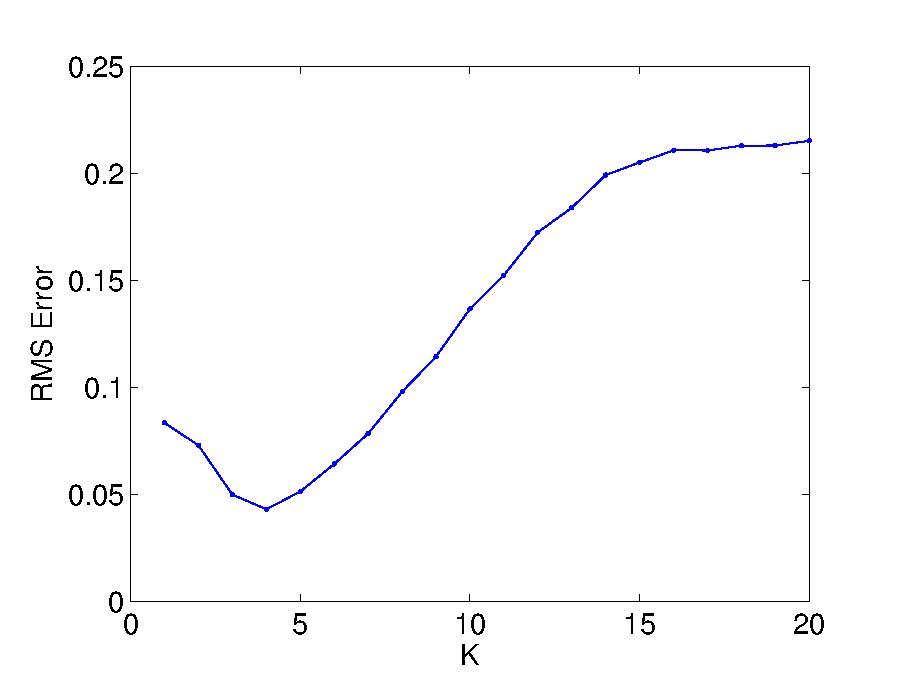
\includegraphics[width=.45\textwidth]{Figures/LLR-nonlinfunction_var_K}
	\label{fig:LLR-K_varying}
	} 
	\subfigure[Locally optimal $K$]{
	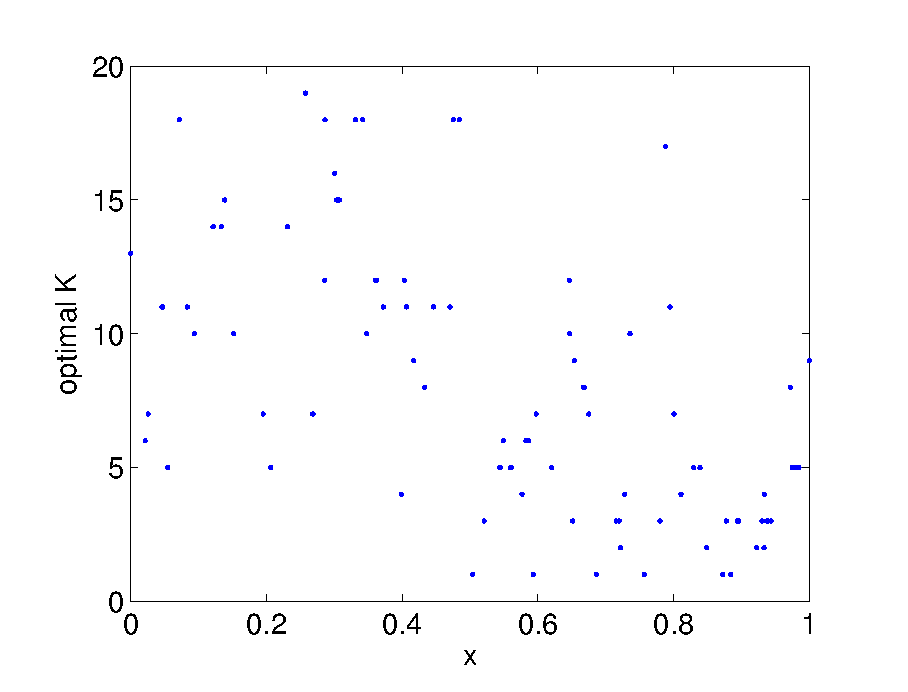
\includegraphics[width=.45\textwidth]{Figures/LLR-nonlinfunction_optimal_K}
	\label{fig:LLR-K_optimal}
	}
	\caption[Global versus local optimal $K$ value]{Comparison between global and local optimal $K$ values for the nonlinear target function \eqnref{eqn:LLR-nonlinear test function}. \subref{fig:LLR-K_varying} shows the \ac{RMS} error of the estimation for a range of different $K$ values. \subref{fig:LLR-K_optimal} shows the locally optimal value of $K$ for a range of $x$ values.}
	\label{fig:LLR-nonlinfunction_K}
\end{figure}

\paragraph{Locally optimal $K$}
A more advanced method of selecting $K$ is choosing a specific value for every query point. Using different values for every query point could lead to a better estimation quality on average. Unfortunately, an analytical formula for finding the optimal value does not exist, since the effect of an single unknown sample on the estimation quality is not known\footnote{Incremental linear regression methods that solve a least squares problem by adding samples one-by-one do exist. However, they do not give an analytical expression for the influence of a single sample on the output or the prediction accuracy.}. Therefore, the locally optimal value has to be found by computing the model for a set of $K$ values and selecting the one that is best according to some quality measure. Notice that this quality measure may only depend on the memory samples and not on the actual output, since this may be unknown. A possible quality measure could be the prediction interval discussed in Section \ref{sec:LLR-prediction interval}. We select the $K$ value that leads to the smallest prediction interval as optimal.

\figref{fig:LLR-K_optimal} shows the locally optimal value for $K$ for the nonlinear test function \eqnref{eqn:LLR-nonlinear test function}. It is clear that the optimal value varies heavily over the domain of the function. On closer inspection, we notice that the optimal value is in general smaller for larger $x$-values. This is due to the faster dynamics of the test function for these values of $x$. For smaller $x$-values the optimal value is larger due to the slower dynamics.
%\begin{figure}[htbp]
%	\centering
%		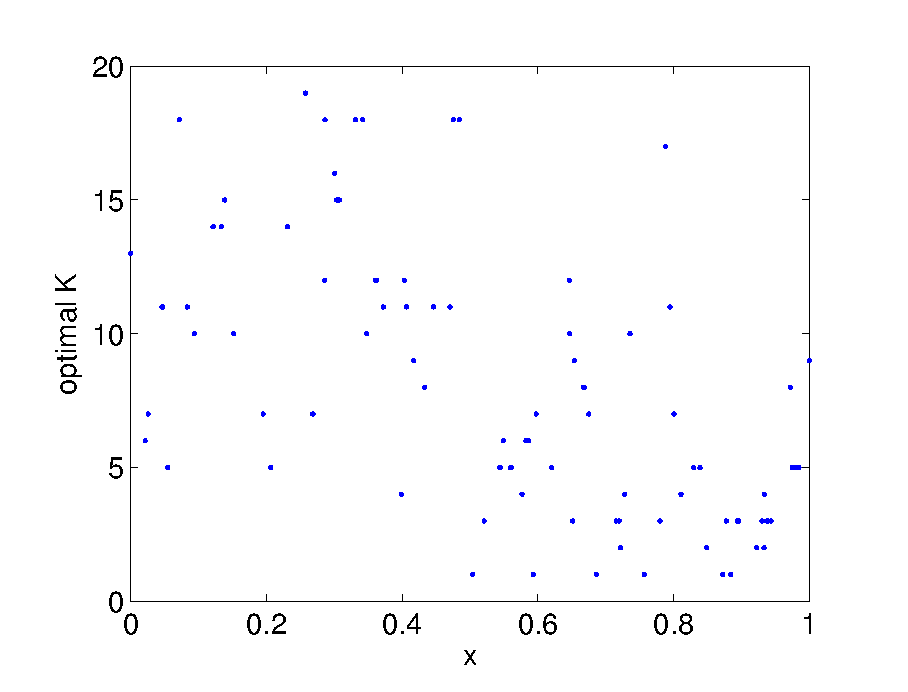
\includegraphics[width=.5\textwidth]{Figures/LLR-nonlinfunction_optimal_K}
%	\caption[Optimal $K$ value]{Locally optimal value of $K$ for the nonlinear test function \eqnref{eqn:\ac{LLR}-nonlinear test function}.}
%	\label{fig:LLR-K_optimal}
%\end{figure}

The difference between a locally and globally optimal value of $K$ is shown in \figref{fig:LLR-nonlinfunction_K_local_global}. The global $K$ value is set to $K=4$. We notice that the prediction interval is smaller using a locally optimal $K$. This is as expected, since this is the quantity we minimized in selecting $K$. However, if we look at the estimated values, the results vary. In high frequency regions (near $x=0.85$ and $x=0.95$) we notice that the estimate improves when a locally optimized $K$ value is used. In low frequency regions (near $x=0.05$ and $x=0.45$ for example), the estimation becomes worse. This is due to the fact that a linear model is fitted to a small number of noisy samples. 

\begin{figure}[htbp]
\centering
\subfigure[Globally fixed $K=4$]{
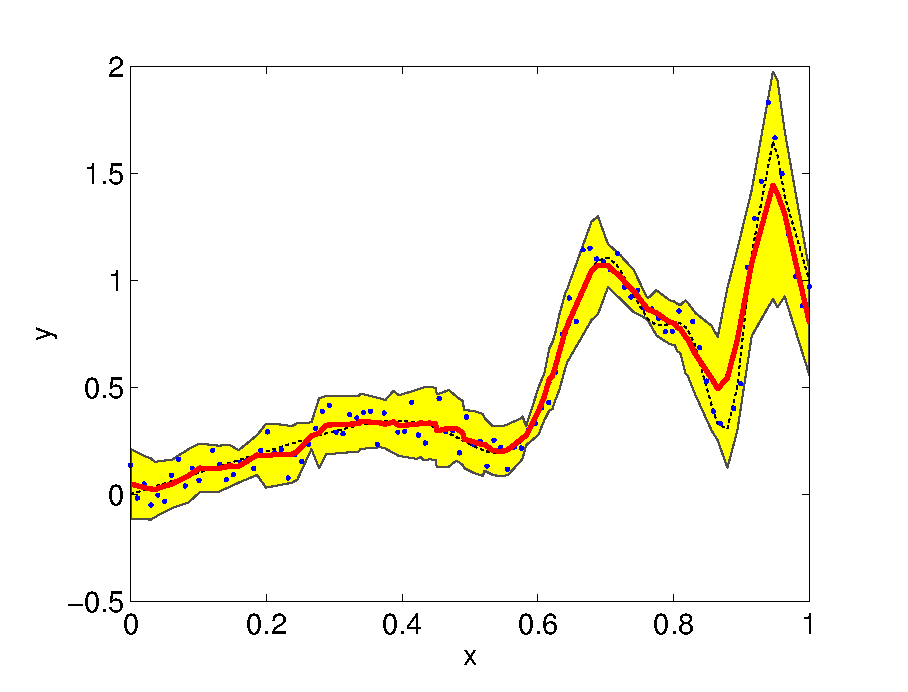
\includegraphics[width=.45\textwidth]{Figures/LLR-nonlinfunction_globalk}
\label{fig:LLR-nonlinfunction_globalk}
} 
\subfigure[Locally optimal $K$]{
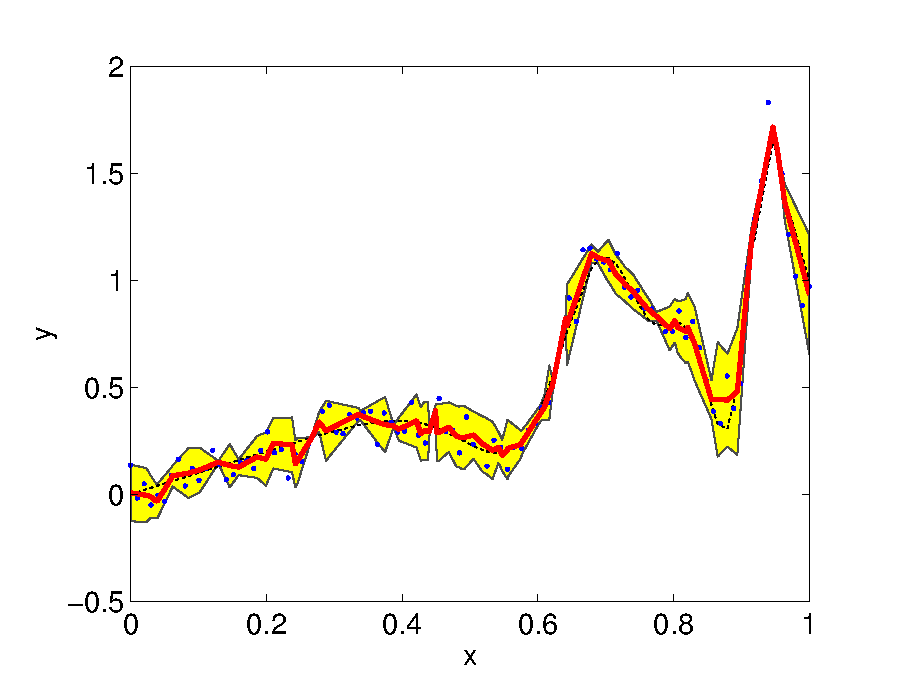
\includegraphics[width=.45\textwidth]{Figures/LLR-nonlinfunction_localk}
\label{fig:LLR-nonlinfunction_localk}
}
\caption[\ac{LLR} estimate of a nonlinear function]{\ac{LLR} estimate (solid red line) of a nonlinear function (dashed line) with prediction intervals (shaded area). \subref{fig:LLR-nonlinfunction_globalk} shows the resulting estimate for a globally optimal (fixed) value of $K$. \subref{fig:LLR-nonlinfunction_localk} shows the result for a locally optimal (varying) value of $K$.}
\label{fig:LLR-nonlinfunction_K_local_global}
\end{figure}

Whether or not a locally optimized $K$-value leads to better estimations than a globally optimized value will depend on the situation. In very noisy applications, using the prediction interval to determine a locally optimal value might lead to bad estimates. A globally optimal $K$ value is probably a good choice is most situations. In the remaining experiments, we selected a globally optimal $K$ value in a way very similar to the approach described in this section. 





\subsection{Two-link manipulator}\label{sec:LLR-two link manipulator}
In this section we will use \ac{LLR} to model state-transitions of a realistic setup. We consider a two-link manipulator system (see \figref{fig:LLR-twolinkmanipulator}). It was chosen because of its relative simplicity and because of its connection with a humanoid robot setup. The manipulator resembles one leg of a humanoid robot, actuated at the knee and hip joints. If this setup leads to good results, it gives confidence that \ac{LLR} might also be used to model a real humanoid robot setup.
\begin{figure}[htbp]
	\centering
		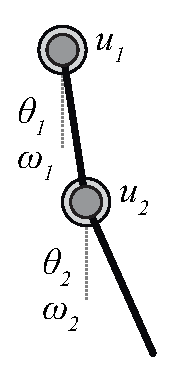
\includegraphics[width=.1\textwidth]{img/twolinkmanipulator}
	\caption[Two-link manipulator setup]{Two-link manipulator setup.}
	\label{fig:LLR-twolinkmanipulator}
\end{figure}

%\paragraph{System}\label{sec:LLR-two link manipulator system}
The two-link manipulator consists of two actuated joints, connected with rigid arms. The system is fixed at one of the joints. The setup is placed vertically. The system has a 4 state-variables: the two angles $\bm{\theta} = \begin{bmatrix} \theta_1 & \theta_2 \end{bmatrix}^T$ and two angular velocities $\bm{\omega} = \begin{bmatrix}\omega_1 & \omega_2 \end{bmatrix}^T$ of both joints. The full state-vector is $\mathbf{x} =  \begin{bmatrix} \bm{\theta} & \bm{\omega} \end{bmatrix}^T$. The input of the system are the output voltages to the motors: \lsymb{$\mathbf{u}$}{Input vector}$ = \begin{bmatrix} u_1 & u_2 \end{bmatrix}^T$. The voltages are limited to $\begin{bmatrix} 1.5 & 1 \end{bmatrix}^T$. The angles are limited to $[-\pi \quad \pi]$. The system is controlled at discrete time intervals $t$, with sampling time $T_s = 0.05$~s. The equations of motion are nonlinear and are given by:
$$
	M(\bm{\theta})\dot{\bm{\omega}}+ C(\bm{\theta}, \bm{\omega}) \bm{\omega} + G(\bm{\theta}) = \mathbf{u}
$$
\begin{eqnarray}
	M(\bm{\theta}) &=& \begin{bmatrix}
	P_1 + P_2 + 2P_3 \cos{\theta_2} & P_2 + P_3 \cos{\theta_2} \\
	P_2 + P_3 \cos{\theta_2} & P_2 \end{bmatrix} \nonumber
	\\
	C(\bm{\theta}, \bm{\omega}) &=& 
	\begin{bmatrix} b_1 - P_3 \omega_2 \sin{\theta_2} & P_3(\omega_1+\omega_2) \sin{\theta_2} \\
	P_3 \omega_2 \sin{\theta_2} & b_2 \end{bmatrix} \nonumber
	\\
	G(\bm{\theta}) &=& \begin{bmatrix} -g_1 \sin{\theta_1}-g_2 \sin{(\theta_1 + \theta_2)} \\
	-g_2 \sin{(\theta_1+\theta_2)} \end{bmatrix} \nonumber
\end{eqnarray}
The abbreviations are defined as follows:
\begin{eqnarray}
	P_1 =& m_1c_1^2 + m_2l_1^2 + I_1 \nonumber \\
	P_2 =& m_2c_2^2 + I_2 \nonumber \\
	P_3 =& m_2l_1c_2 \nonumber \\
	g_1 =& (m_1c_1 + m_2l_1)g \nonumber \\
	g_2 =& m_2c_2g \nonumber
\end{eqnarray}
The parameters of the system and their physical meanings can be found in \tabref{tab:LLR-two link manipulator parameters}.
\begin{table}[htbp]
	\centering
	\caption[Two-link manipulator: Parameter values]{Physical parameters of the two-link manipulator}
		\begin{tabular}{ll}
			Symbol & Parameter \\ \hline
			$g = 9.81 \textrm{ m/s}^2$ & gravitational acceleration \\
			$l_1 = 0.4$ m & length of first link \\
			$l_2 = 0.4$ m & length of second link \\
			$m_1 = 1.25$ kg & mass of first link \\ 
			$m_2 = 0.8$ kg & mass of second link \\
			$I_1 = 0.07 \textrm{ kgm}^2$ & inertia of first link \\ 
			$I_2 = 0.04 \textrm{ kgm}^2$ & inertia of second link \\ 
			$c_1 = 0.2$ m & center of mass of first link \\
			$c_2 = 0.2$ m & center of mass of second link \\
			$b_1 = 0.08$ kg/s & damping in first joint \\
			$b_2 = 0.02$ kg/s & damping in second joint
		\end{tabular}
	\label{tab:LLR-two link manipulator parameters}
\end{table}

%\subsubsection{Experimental setup}\label{sec:LLR-two link manipulator experimental setup}
The model was implemented as a simulation in Matlab. A white noise signal with $\sigma^2 = 0.01$ was added to each output. The following input-output relation was estimated:
$$
	\hat{\mathbf{x}}_{t+1} = \begin{bmatrix} \mathbf{x}_t \\ \mathbf{u}_t \\ 1 \end{bmatrix}^T \hat{\bm{\beta}}
$$
with $\hat{\bm{\beta}}$ the local linear model. A dataset was generated by applying a random input signal to the system and observing the resulting state-transitions for 250 seconds (5000 samples). The memory was filled with state-transition samples: $(\mathbf{x}_t,\mathbf{u}_t,\mathbf{x}_{t+1})$. The number of nearest neighbors used in the experiments was fixed to $K=10$.

The two-link manipulator setup was used to investigate some of the properties of the \ac{LLR} method in a setting that resembles a real learning experiment. We are mainly interested in the ability of \ac{LLR} to model state-transitions and the influence of the memory size on the estimation accuracy. Furthermore, we are interested if fitting a linear model to a set of nearest neighbors improves the estimation compared to more simpler memory-based methods. We can summarize these questions as follows:
\begin{enumerate}
	\item Can \ac{LLR} be used to model state-transitions?
	\item How does the memory size influence the estimation accuracy?
	\item Is \ac{LLR} an improvement over other memory-based methods?
\end{enumerate}



%\subsubsection{Results}\label{sec:LLR-two link manipulator results}
\subsubsection{Estimating state-transitions}\label{sec:LLR-2link_statetransitions}
\begin{figure}[htbp]
	\centering
	\subfigure[Memory size: $N=200$ (10 s)]{
		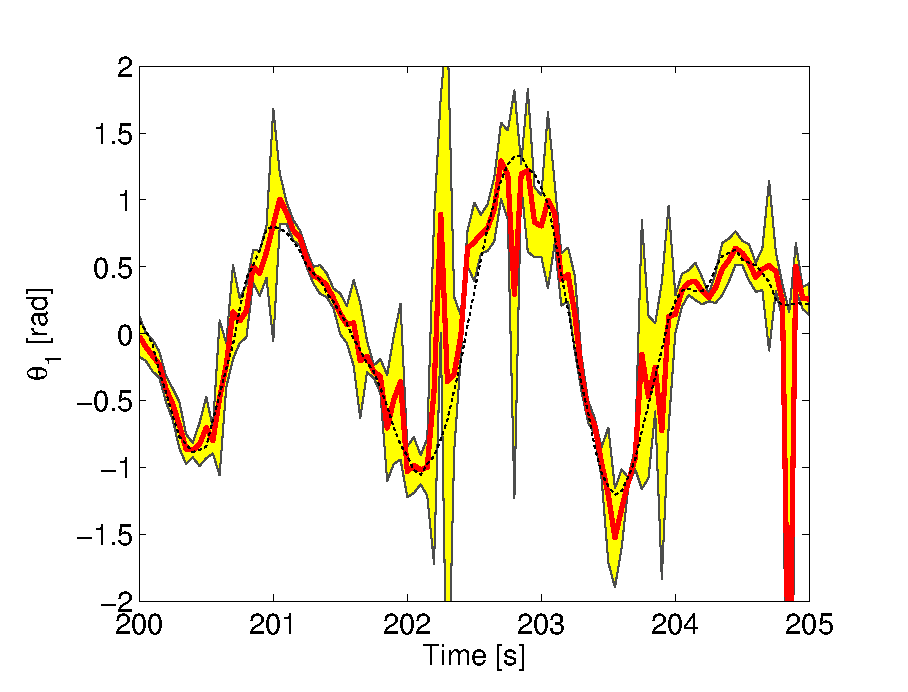
\includegraphics[width=.4\textwidth]{Figures/LLR-robotarm_theta1}
		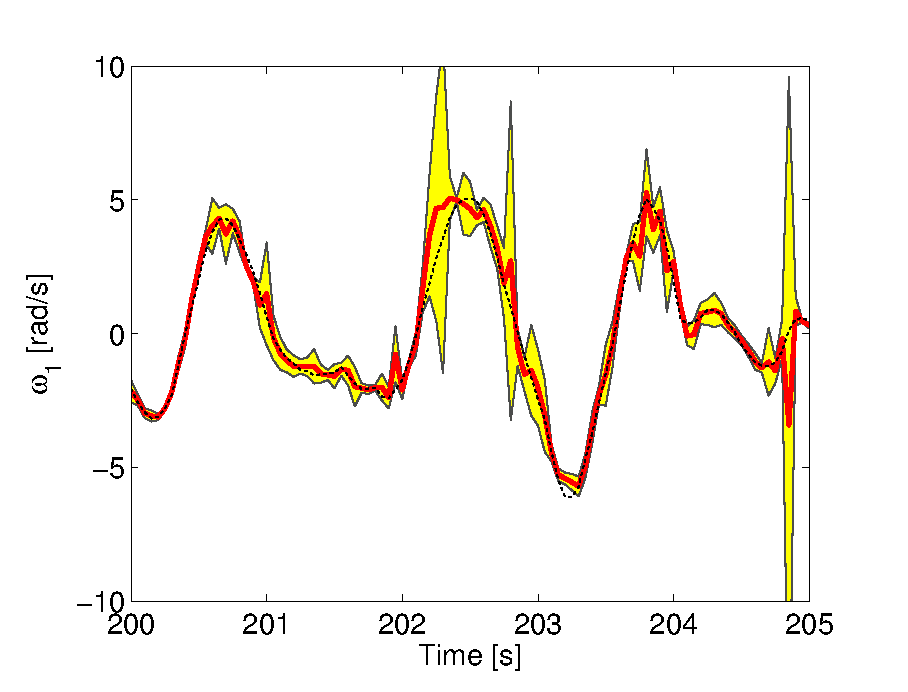
\includegraphics[width=.4\textwidth]{Figures/LLR-robotarm_omega1}
		\label{fig:LLR-RobotarmIncr_N1}
	}\\
	\subfigure[Memory size: $N=4000$ (200 s)]{
		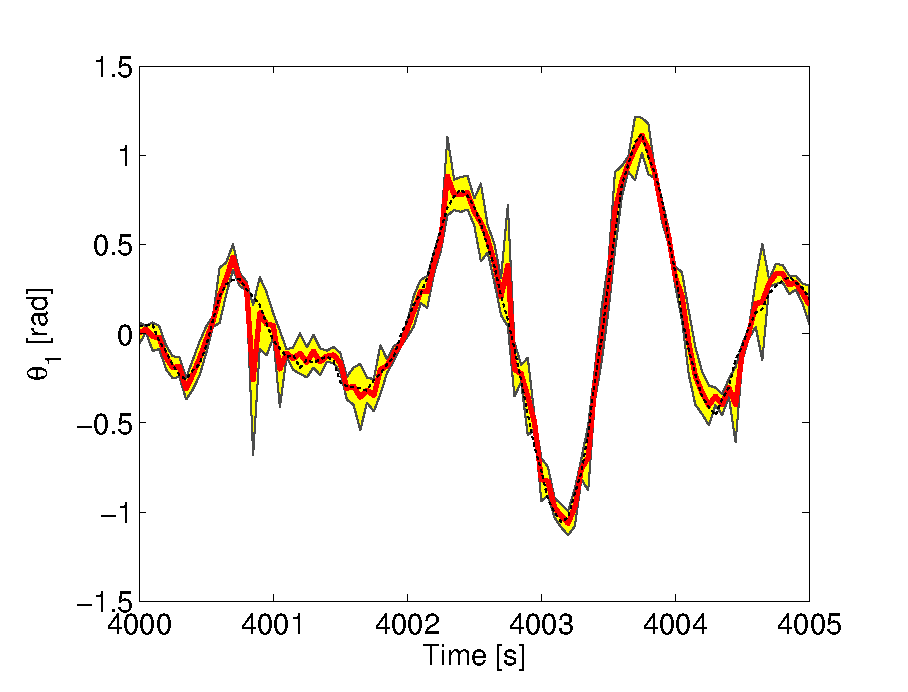
\includegraphics[width=.4\textwidth]{Figures/LLR-robotarm_theta2}
		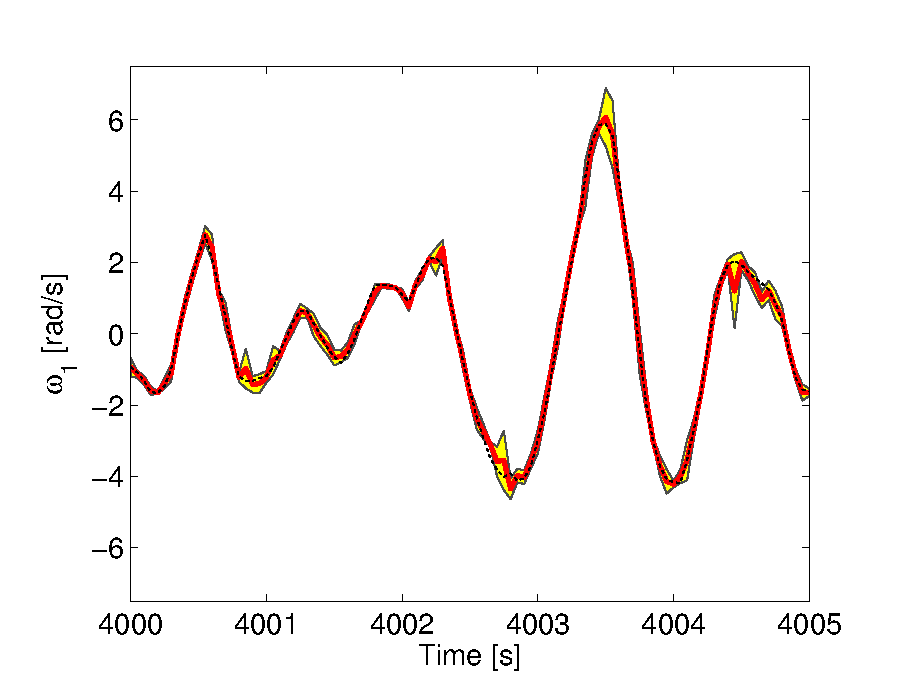
\includegraphics[width=.4\textwidth]{Figures/LLR-robotarm_omega2}
		\label{fig:LLR-RobotarmIncr_N2}
	}
	\caption[\ac{LLR} estimate of the two-link manipulator]{\ac{LLR} estimate of state-transitions for the two-link manipulator for increasing memory size using $K=10$. The figures show the improvement of the \ac{LLR} estimate for $\theta_1$ (left figures) and $\omega_1$ (right figures). \subref{fig:LLR-RobotarmIncr_N1} is the estimate using a memory of size $N=200$ (10 seconds), \subref{fig:LLR-RobotarmIncr_N2} the estimate for $N=4000$ (200 seconds). The figures show the \ac{LLR} estimate (red solid line), the measured value (black dashed line) and the prediction intervals (shades areas).}
	\label{fig:LLR-RobotarmIncr}
\end{figure}
In a typical real-world learning experiment, the size of the memory available to the model increases during the experiment. We mimic this situation by increasing the size of the memory available to the \ac{LLR} algorithm. At every time step, the model uses the memory samples observed up until that moment. These memory samples are used to estimate the transition from the current state to the next. We expect that the estimations become better with increasing memory size. \figref{fig:LLR-RobotarmIncr} shows the estimated state-transitions at two moments in the experiment for the angle $\theta_1$ and angular velocity $\omega_1$ of the first link. The state-variables of the second link show the same behavior and are therefore not shown. 

The first observation that has to be made, is the fact that \ac{LLR} is indeed able to model state-transitions. Using state-action pairs as input, the resulting next state can be estimated as output. Especially with a large memory (\figref{fig:LLR-RobotarmIncr_N2}), the estimated state-transitions closely match the real state-transitions. It appears that the prediction intervals can be used as a measure for the estimation accuracy. We notice that state-transitions that are estimated inaccurately, also have a relatively large prediction interval. Especially with a large memory, the prediction intervals are small compared to the amplitude of the variables. 

The improvement of the estimate with increasing memory size, is also visualized in \figref{fig:LLR-robotarm_RMSE_compare}. The figure shows the RMS error of the estimated state-transitions. The estimation improves with the first 1000 samples and is more or less equal thereafter.
\begin{figure}[htbp]
	\centering
		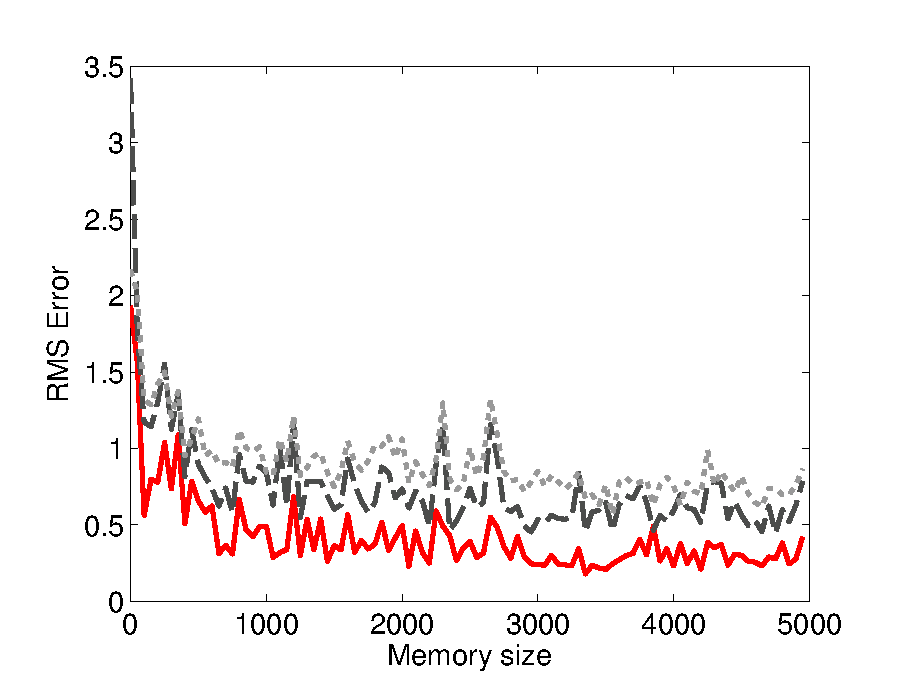
\includegraphics[width=0.5\textwidth]{Figures/LLR-robotarm_RMSE_compare}
		\caption[Estimation error for the two-link manipulator for increasing memory size]{\ac{RMS} estimation error for increasing memory size using different methods to estimate the two-link manipulator. The figure compares the nearest neighbor estimate ($K=1$, dotted gray line), the $K$ nearest neighbors average ($K=10$, dashed gray line) and the \ac{LLR} estimate ($K=10$, solid red line).}
	\label{fig:LLR-robotarm_RMSE_compare}
\end{figure}


%\paragraph{Comparing model-based modeling methods} 
\subsubsection{Comparing memory-based modeling methods}\label{sec:LLR-2link_ModelBasedComparison}

\begin{figure}[htbp]
	\centering
		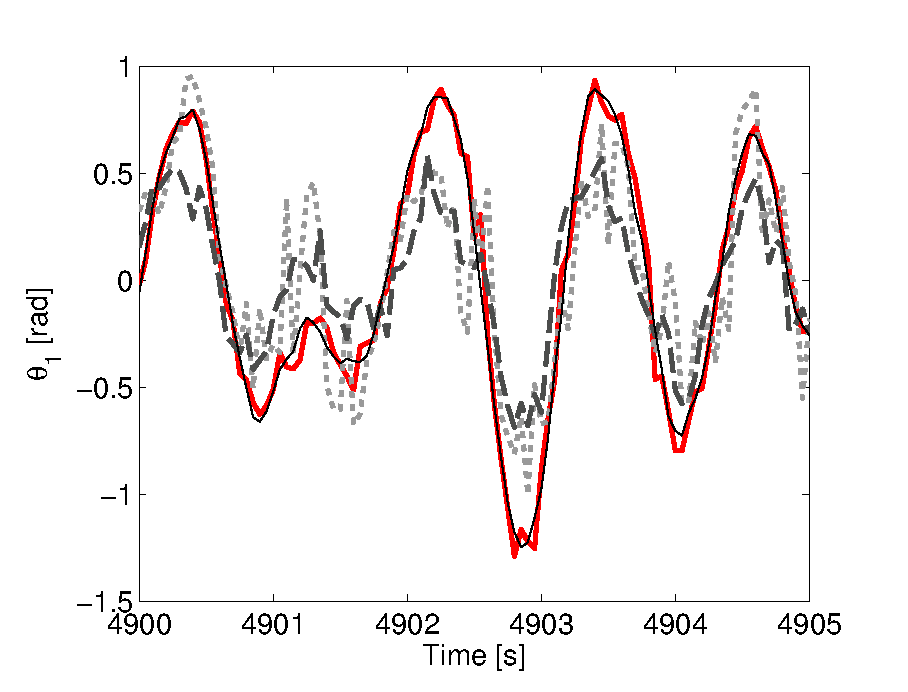
\includegraphics[width=0.5\textwidth]{Figures/LLR-robotarm_trajectory}
		\caption[Comparing three memory-based modeling methods]{Comparison of three memory-based modeling methods on the two-link manipulator using a large memory ($N=5000$). The figure shows the estimation of a trajectory (solid black line) using the nearest neighbor ($K=1$, dotted gray line), the $K$ nearest neighbors average ($K=10$, dashed gray line), and the \ac{LLR} estimate ($K=10$, solid red line).}
	\label{fig:LLR-robotarm_trajectory}
\end{figure}
We have introduced \ac{LLR} as a memory-based modeling method that fits a linear model to the set of nearest neighbors around the query input. Linear regression is a time consuming process, so the question rises whether fitting a linear model to the set of nearest neighbors is needed. Instead of estimating a model, we could also use the average output of the nearest neighbors as estimate (the $K$ nearest neighbors average). An even faster option is to simply use the output of the nearest neighbor ($K=1$) as an estimation for the output.
 
\figref{fig:LLR-robotarm_trajectory} compares these three memory-based methods by estimating a 5-second trajectory using a random input signal and a large memory ($N=5000$) to estimate state-transitions. We see that over the entire trajectory the \ac{LLR} method outperforms the other memory-based methods. It seems that the other methods give an estimate that is too conservative. \figref{fig:LLR-robotarm_RMSE_compare} confirms this by showing that the \ac{RMS} estimation error of \ac{LLR} is smaller than the other memory-based methods for all memory sizes. \figref{fig:LLR-robotarm_trajectory} shows that the difference in estimation quality is significant, so we conclude that fitting a linear model to the set of nearest neighbors leads to much better state-transition estimates. We argue that the improvement in estimation quality is worth the extra computational effort needed to estimate the linear model.








\subsection{Humanoid robot}\label{sec:LLR-robot leo}
In this section we use a two-legged humanoid robot called `Leo' as experimental setup. Leo is a humanoid robot developed at Delft University as a test platform to perform \ac{RL} experiments (\figref{fig:LLR-Leo}). It was designed to be able to walk autonomously in circles. It is connected via a boom construction to a central rotating pivot, so it can theoretically walk infinitely long in circles. It has an arm that makes it possible to stand up when fallen. The setup is highly complex and is usable for performing advanced reinforcement learning experiments. We use it as a setup to test the ability of \ac{LLR} to model complex, real-world systems.
\begin{figure}[htbp]
	\centering
		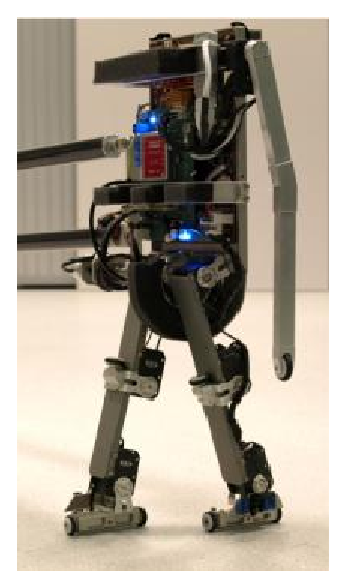
\includegraphics[width=.2\textwidth]{img/leo1}
	\caption[Humanoid robot setup]{Two-legged humanoid robot 'Leo'.}
	\label{fig:LLR-Leo}
\end{figure}
The robot is actuated at its angles, knees and hips. The motors also act as sensors that measure angle and angular velocity. Apart from the actuators, there are also sensors in the feet (that detect whether or not a foot touches the ground) and in the boom construction (measuring angle and angular velocity of the torso). In total, the robot has got 18 state-variables and 6 inputs. The states are concatenated in a $1\times 18$ row vector $\mathbf{x}$ and the actions in a $1\times 6$ row vector $\mathbf{u}$. The \ac{LLR} model $\hat{\bm{\beta}}$ estimates the state-transition from a state $\mathbf{x}_t$ to the next state $\mathbf{x}_{t+1}$ when actuated with action $\mathbf{u}_t$: 
$$
	\hat{\mathbf{x}}_{t+1} = \begin{bmatrix} \mathbf{x}_t \\ \mathbf{u}_t \\ 1 \end{bmatrix}^T \hat{\bm{\beta}}
$$

%\subsubsection{Experimental setup}\label{sec:LLR-robot leo experimental setup}
A large number of memory samples was gathered by letting Leo walk for about two minutes sampling at $150$~Hz using a pre-programmed controller. Although the walking motion looks to be the same in every step, closer inspection of the data reveals differences in every step (due to variations in the floor and other disturbances). The total dataset was split into two parts (both consisting of 8000 samples): one set for estimating the model and one for validating it. We used $K = 40$ for all Leo experiments. This value was determined empirically to give satisfactory results.

We have used \ac{LLR} to model this system to investigate its performance on modeling complex systems. The questions to be answered are:
\begin{enumerate}
	\item Can \ac{LLR} be used to model a complex, high-dimensional system?
	\item How large does the memory need to be for a reasonable estimation?
\end{enumerate}


%\subsubsection{Results}\label{sec:LLR-robot leo results}

%\paragraph{Modeling with large memory}
\subsubsection{Modeling walking motion}\label{sec:LLR-Leo_FullMemory} 
To show that the \ac{LLR} method is able to accurately model a high-dimensional system, we estimated the state-transitions of the validation dataset. The \ac{LLR} estimates were determined using the estimation dataset ($N=8000$) as memory. \figref{fig:LLR-LeoFullMemStep} shows the response of the real system and its \ac{LLR} estimate of one stride (two steps). For clarity we do not show all 18 state-variables but only the torso, the left hip and left foot (the estimates of all 18 state-variables can be found in Appendix \ref{app:LeoWalking}). We show these three variables, since they represent the remaining state-variables very well. Furthermore, since all estimated steps in the dataset are estimated approximately equally good, we show only one stride. 

We notice that in all three cases the output is estimated very accurate. In fact, the measured states are barely visible due to the very close estimates of the \ac{LLR} model. Also the prediction intervals are small (especially for the torso and the left hip), which indicates that the estimates are based on sets of very linear data. Although all variables are estimated accurately, the torso angle is clearly estimated best and the foot contact worst. This is reflected by the prediction intervals, which are small for the torso and hip, but larger for the foot. The main reason for this, is that the foot sensor data is very noisy. This is also visible from inspection of the measured data. 


\begin{figure}[htbp]
\centering
\subfigure[Torso angle]{
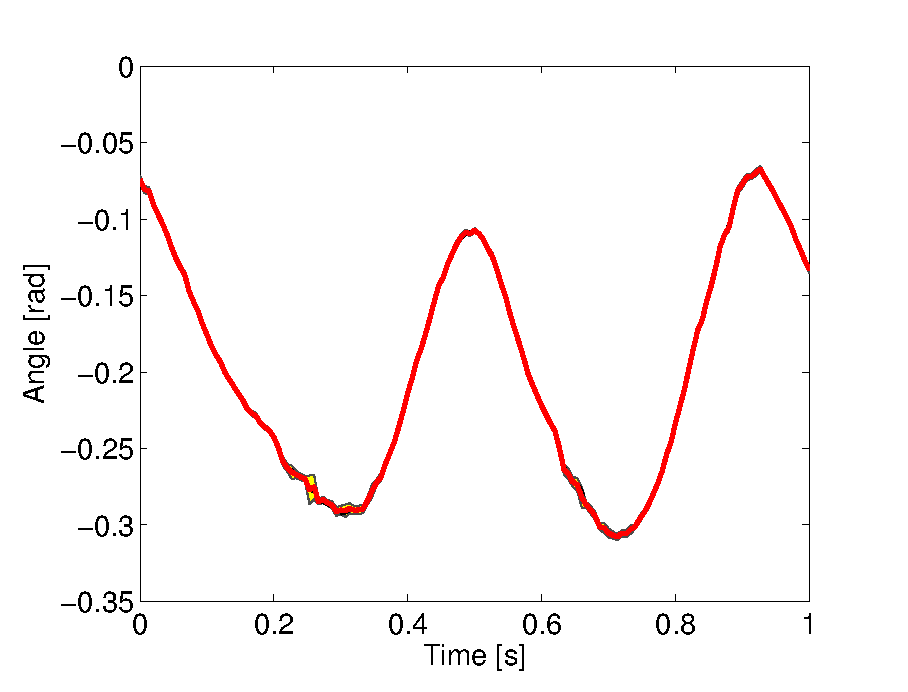
\includegraphics[width=.3\textwidth]{Figures/LLR-LeoFullMemStep_Torso}
\label{fig:LLR-LeoFullMemStep_Torso}
}
\subfigure[Left hip angle]{
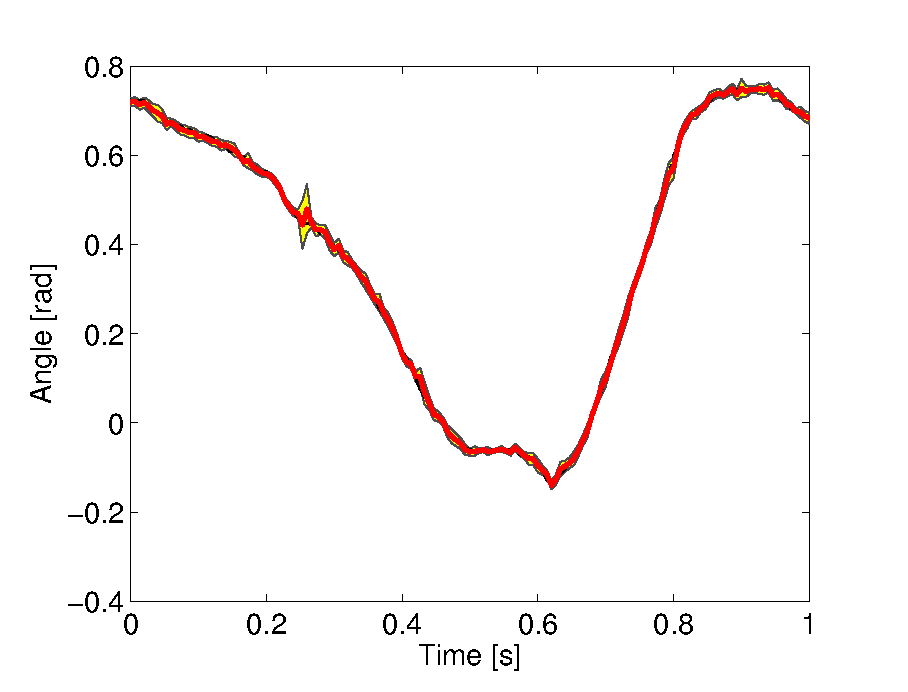
\includegraphics[width=.3\textwidth]{Figures/LLR-LeoFullMemStep_HipLeft}
\label{fig:LLR-LeoFullMemStep_HipLeft}
}
\subfigure[Left foot contact]{
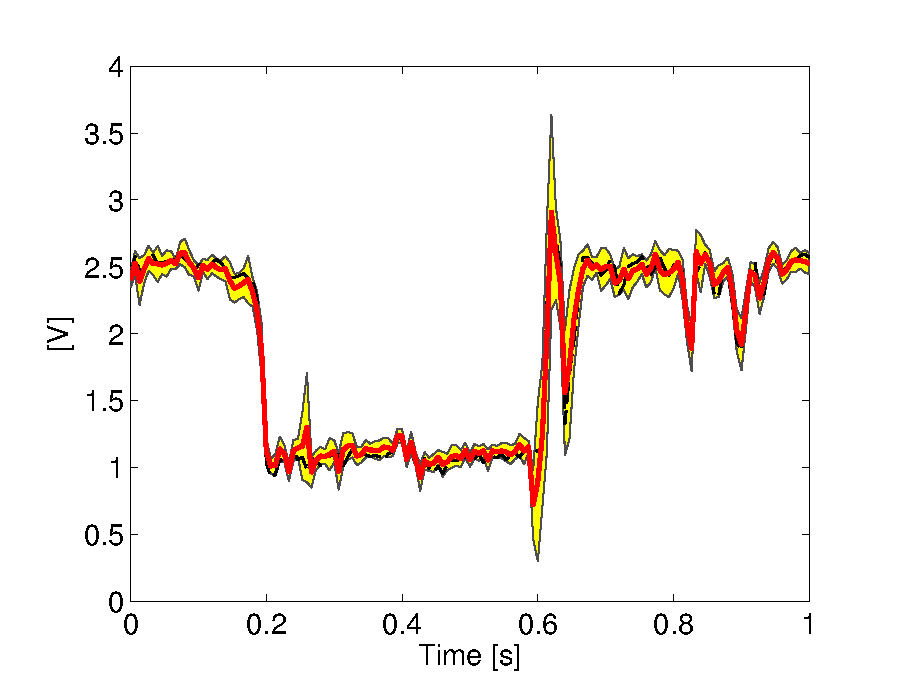
\includegraphics[width=.3\textwidth]{Figures/LLR-LeoFullMemStep_Foot}
\label{fig:LLR-LeoFullMemStep_Foot}
} 
\caption[\ac{LLR} estimate of Leo walking]{\ac{LLR} estimate ($K=40$) of the walking motion of robot Leo using a memory consisting of 8000 samples. Three of the total of 18 state-variables are shown for one stride (two steps). \subref{fig:LLR-LeoFullMemStep_Torso} shows the angle of the torso, \subref{fig:LLR-LeoFullMemStep_HipLeft} shows the angle of the left hip, \subref{fig:LLR-LeoFullMemStep_Foot} the voltage of the left foot sensor. The figures show the \ac{LLR} estimate (solid red line), the measured output (dashed black line) and the prediction interval (shaded area).}
\label{fig:LLR-LeoFullMemStep}
\end{figure}

%\paragraph{Modeling with increasing memory} 
\subsubsection{Modeling using increasing memory}\label{sec:LLR-Leo_IncrMemory} 
In order to see the effect of the memory size on the estimation quality, we will again estimate the walking motion, but this time using a memory that increases in size. Starting with an empty memory, a new sample from the estimation dataset is added to the memory at every time step. This resembles a learning experiment which is started from no initial knowledge about the environment, but acquires one new state-transition at every time step.

\figref{fig:LLR-LeoIncrMemStep} shows the improvement of the \ac{LLR} estimate for state-variables torso angle, left hip angle and left foot contact. We show the \ac{LLR} estimates of the three variables for increasing memory size. The torso angle and left hip angle are estimated quite accurately, even from a very small number of memory samples. This is probably due to the similarity between different footsteps for these variables. On the other hand, the foot contact variable is estimated relatively badly, particularly for a small number of memory samples. This is visualized by the bad estimates and the large prediction intervals. As noted before, the bad estimate of the foot sensor is probably due to the noisy and therefore unpredictable behavior of this variable.
 
\figref{fig:LLR-LeoIncrMemError} shows the \ac{RMS} error of the estimation for an increasingly large memory. The estimation error variates during a step. In order to obtain a more smooth graph, we averaged the \ac{RMS} value over an estimated step (about $0.5$~s). So, the graph shows the average \ac{RMS} error of about 100 estimated steps. As expected, we see that the estimation error decreases with increasing memory size. The error decreases up to approximately $N = 2000$ and is more or less constant thereafter. This is approximately equal to 13 strides. So the \ac{LLR} method is able to estimate future steps accurately from 26 previously observed steps. Along with the RMS error of the estimation, we also plotted the \ac{RMS} value of the prediction interval. We notice that the prediction interval has a remarkably similar shape. Because the prediction interval can be considered as  a measure of linearity, this indicates that the size of the estimation error can be related to the nonlinearity of the memory samples. This is a direct consequence of the lack of appropriate nearest neighbors, which then leads to an inaccurate estimate of the state-transition for a particular state-action pair.

Although walking seems to be a motion that is the same in every step, in practice every single step is slightly different due to small disturbances such as ground level variations. This is reflected by sudden increases in the estimation error, for example around $N=4500$. Apparently this step was very different from the previously observed steps and the lack of appropriate nearest neighbors led to a \ac{LLR} estimate that is much worse than for previously estimated steps. This is confirmed by comparing the actual measurements of this step to other steps.

\begin{figure}[htbp]
\centering
\subfigure[Memory size: $N=150$ (2 steps)]{
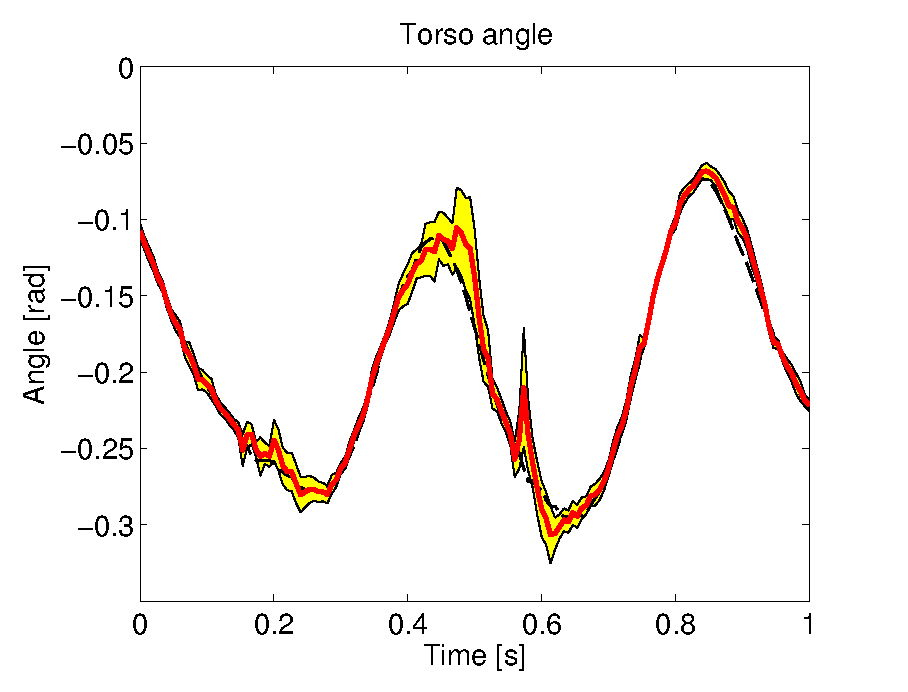
\includegraphics[width=.3\textwidth]{Figures/LLR-LeoIncrMemStep_Torso1}
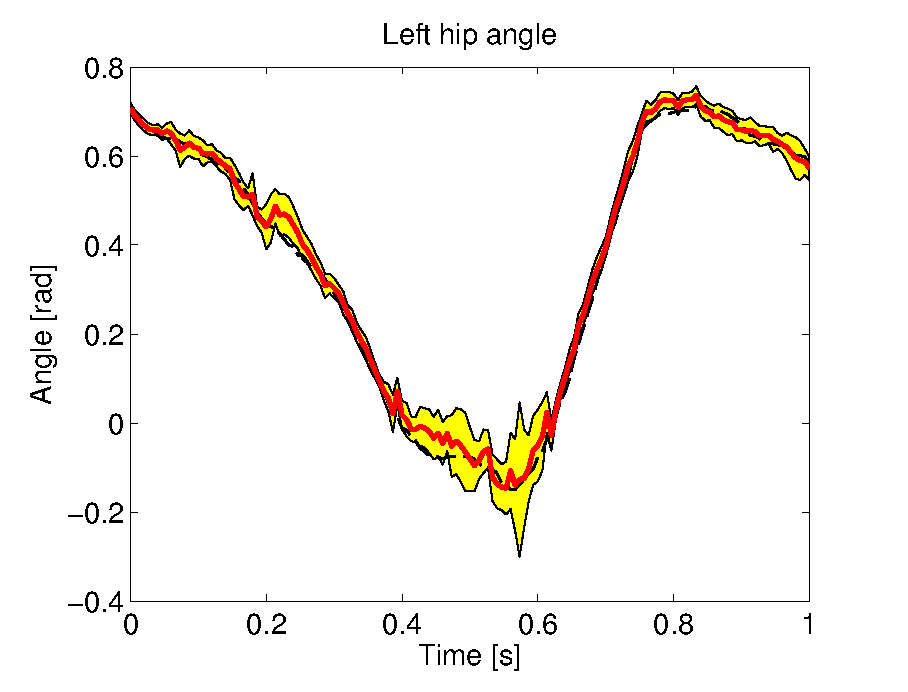
\includegraphics[width=.3\textwidth]{Figures/LLR-LeoIncrMemStep_HipLeft1}
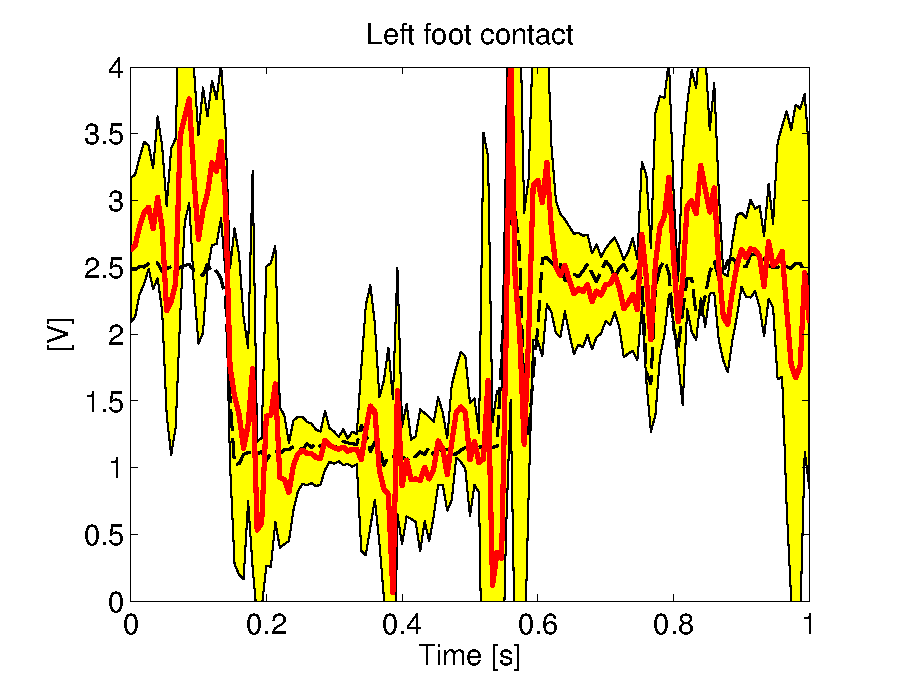
\includegraphics[width=.3\textwidth]{Figures/LLR-LeoIncrMemStep_Foot1}
\label{fig:LLR-LeoIncrMemStep_N1}
}\\
\subfigure[Memory size: $N=1000$ (14 steps)]{
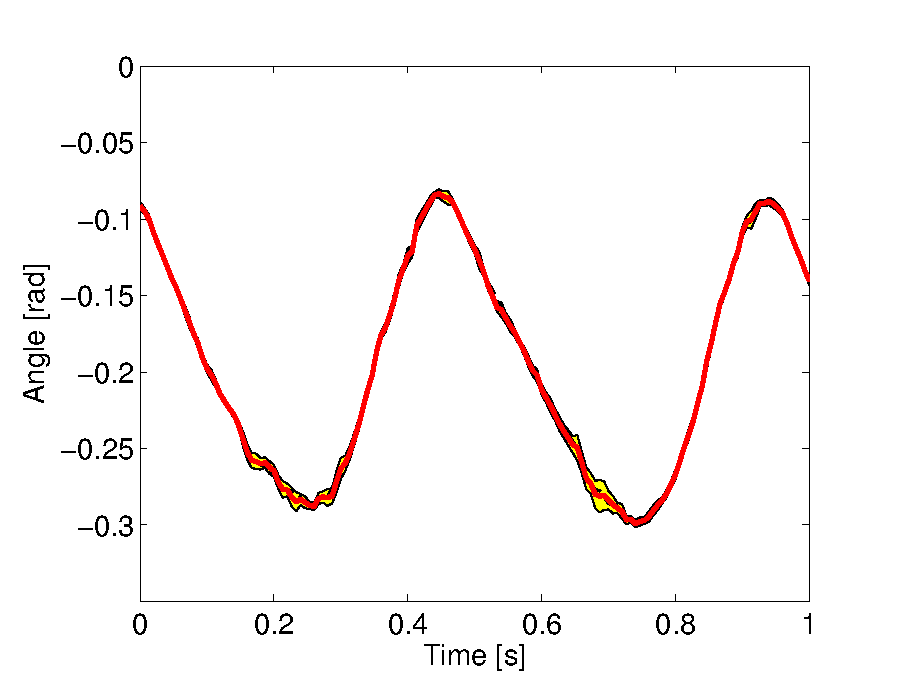
\includegraphics[width=.3\textwidth]{Figures/LLR-LeoIncrMemStep_Torso2}
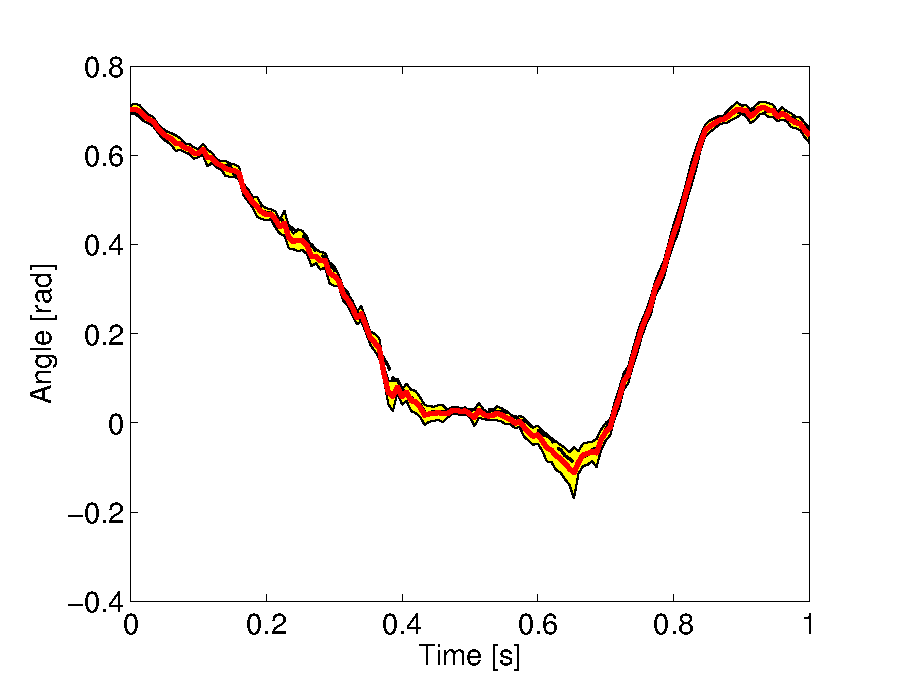
\includegraphics[width=.3\textwidth]{Figures/LLR-LeoIncrMemStep_HipLeft2}
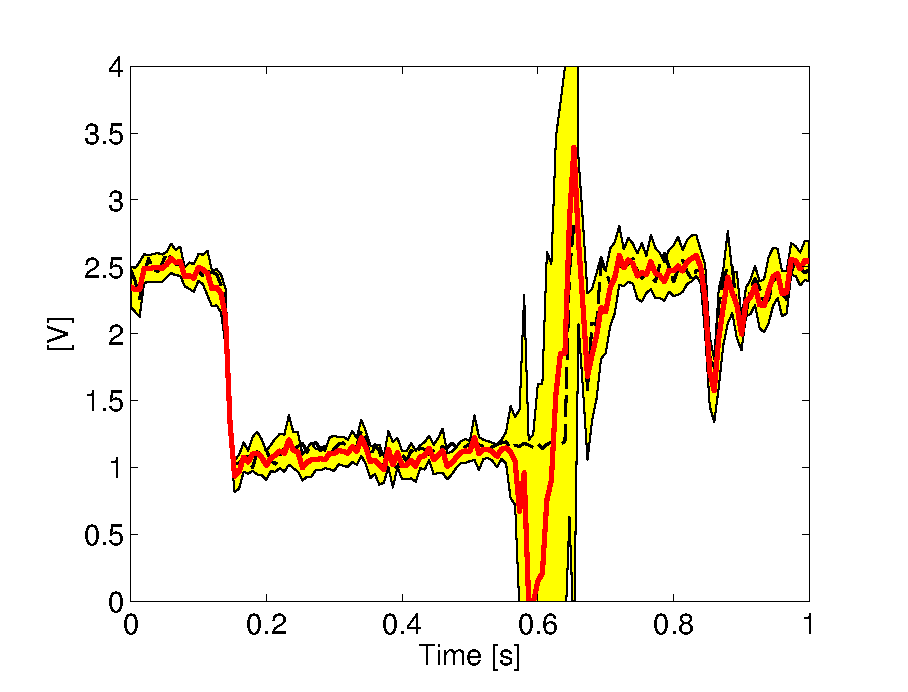
\includegraphics[width=.3\textwidth]{Figures/LLR-LeoIncrMemStep_Foot2}
\label{fig:LLR-LeoIncrMemStep_N2}
}\\
\subfigure[Memory size: $N=6000$ (80 steps)]{
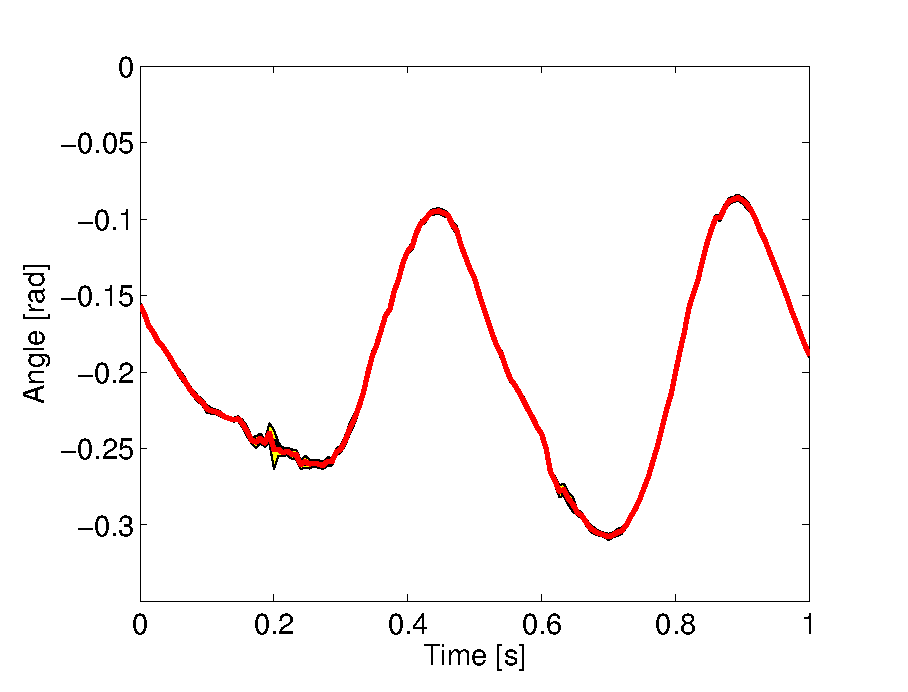
\includegraphics[width=.3\textwidth]{Figures/LLR-LeoIncrMemStep_Torso3}
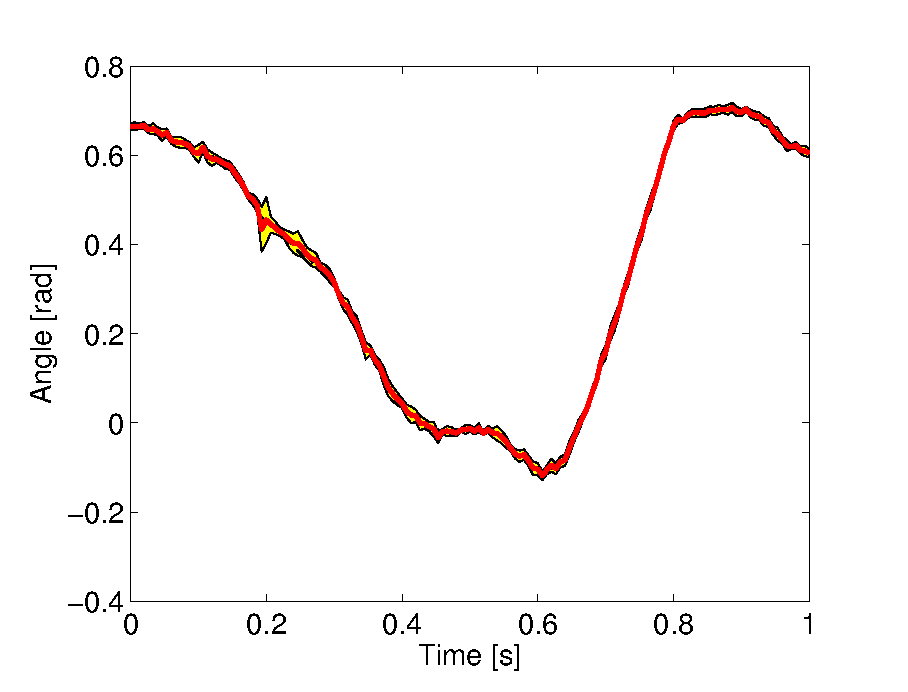
\includegraphics[width=.3\textwidth]{Figures/LLR-LeoIncrMemStep_HipLeft3}
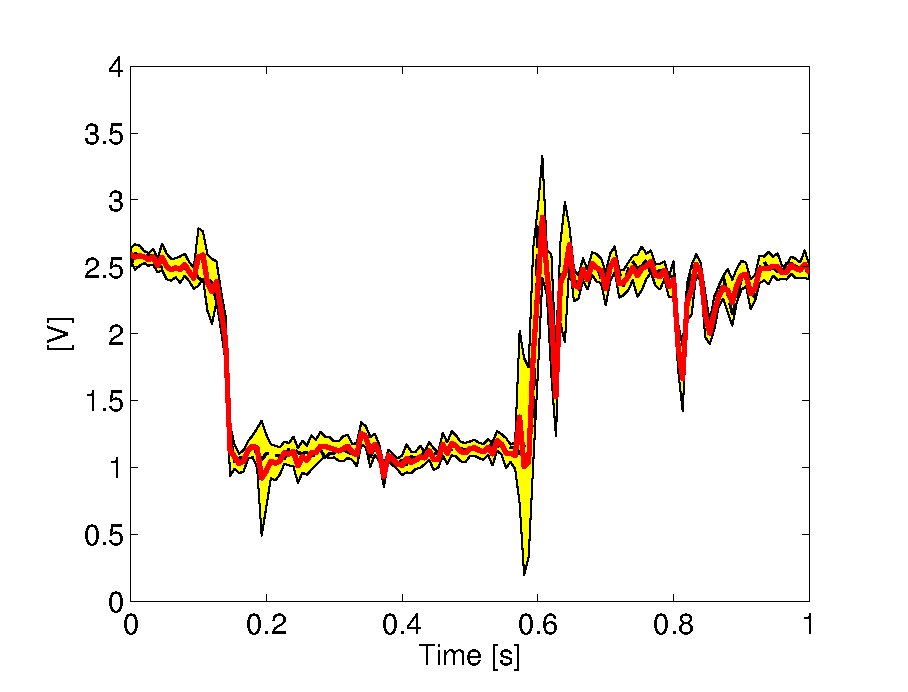
\includegraphics[width=.3\textwidth]{Figures/LLR-LeoIncrMemStep_Foot3}
\label{fig:LLR-LeoIncrMemStep_N3}
} 
\caption[\ac{LLR} estimate of Leo walking for increasing memory size]{Improvement of the \ac{LLR} estimate ($K=40$) of the walking motion of Leo when the memory size increases. The figures show the improvement of the \ac{LLR} estimate for the torso (left), the left hip (middle) and the left foot (right). \subref{fig:LLR-LeoIncrMemStep_N1} is the estimate for a memory of size $N=150$ (roughly 2 steps), \subref{fig:LLR-LeoIncrMemStep_N2} the estimate for $N=1000$ (14 steps) and \subref{fig:LLR-LeoIncrMemStep_N3} for $N=6000$ (80 steps). The figures show the \ac{LLR} estimate (solid red line), the measured value (dashed black line) and the prediction interval (shaded area).}
\label{fig:LLR-LeoIncrMemStep}
\end{figure}

\begin{figure}[htbp]
	\centering
		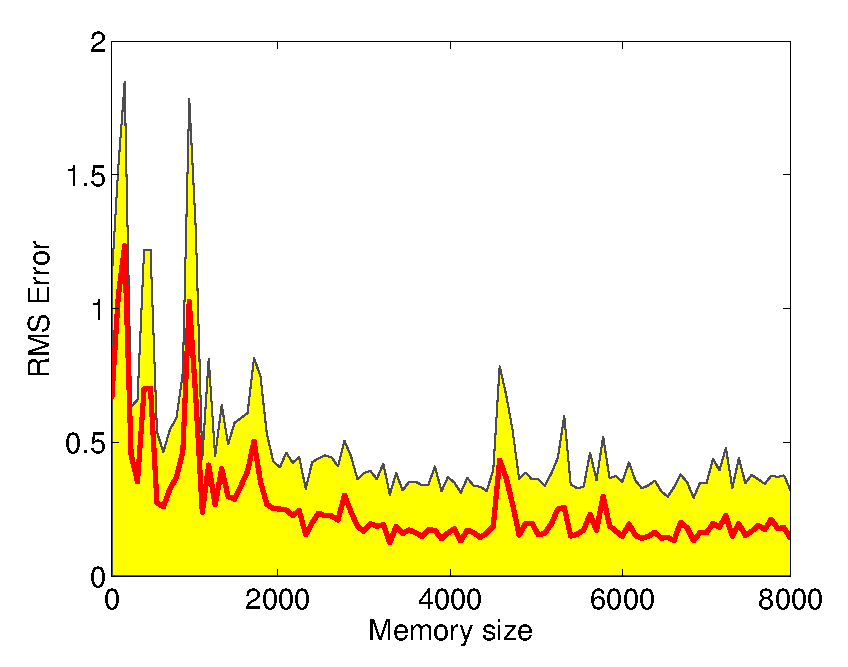
\includegraphics[width=.5\textwidth]{Figures/LLR-LeoIncrMemError}
	\caption[Estimation error for robot Leo for increasing memory size]{\ac{RMS} value of the \ac{LLR} estimation error (solid red line) for the walking motion of Leo for increasing memory size. The shaded area is the \ac{RMS} value of the prediction interval.}
	\label{fig:LLR-LeoIncrMemError}
\end{figure}

%\paragraph{Backwards model} Show that the model can be used in reverse order (using $x_t$ as input and $x_{t-1}$ as output) 






\section{Conclusions}\label{sec:LLR-conclusion}
In this chapter we have introduced \acl{LLR} as method for estimating a model from a set of observed state-transitions. Being a memory-based method, it is easy to implement several results from statistical analysis. Although the number of statistical quantities is vast, we have only described prediction intervals and outlier detection which could be useful in a reinforcement learning setting. In order to decrease the computation time, we introduced a $k$d-tree as a structure to store the samples in the memory. We have shown how the tree structure can be used to search for nearest neighbors more efficiently than a standard sorting approach. 

The capabilities of the \ac{LLR} method were shown in different settings. We used a 1-dimensional nonlinear function to research the possibility to increase the prediction accuracy. We showed that optimizing the number of nearest neighbors locally, can in some cases reduce the estimation error. Also outlier detection was able to identify spikes in the data and resulted in better estimates by neglecting these faulty samples. However, the extra computational effort that is needed to improve the estimate only slightly, makes it not interesting for on-line usage. The prediction interval is a measure for the linearity in the points used in the linear regression and can therefore be used as a rough estimate of the uncertainty in the prediction. 

We applied \ac{LLR} on a two-link manipulator simulation to test its ability to estimate state-transitions. We showed that \ac{LLR} is indeed usable for estimating state-transitions accurately. As expected, increasing the number of samples in the memory, led to an improvement in the estimation accuracy. Furthermore, we showed that fitting a linear model to the set of nearest neighbors (as is done in \ac{LLR}) makes the estimation more accurate compared to memory-based methods that use the average or the nearest neighbor as output.

An important question was whether the \ac{LLR} modeling method still performed well on a complex, noisy system. We answered this question by applying \ac{LLR} on a complex, humanoid robot setup. The \ac{LLR} method proved to be able to model the walking motion of the robot accurately using a relatively small memory of a few thousand samples. One reason that the model is accurate lies in the fact that in all experiments the estimation and validation data are in the same region of state-space. Although this might seem to be an overly ideal situation, this is in fact a reasonable imitation of a real learning process. Not all parts of the state-space are expected to be equally important and we suspect that a perfect model is not needed in all parts, but mainly along trajectories that lead to goal states.

In this chapter, the accuracy of a model was only determined by looking at the response of the model compared to the real system and by inspecting the prediction intervals. The important question whether or not a model is accurate enough to be used in a \ac{RL} setting is deferred to the next chapter where it will be discussed in more detail. 



\chapter{Model-learning RL}\label{chap:Prioritized Sweeping}

\section{Introduction}\label{sec:PS-introduction}
In this chapter, we combine \ac{LLR} with \ac{RL}. We use the \ac{LLR} method as developed and investigated in Chapter \ref{chap:Modeling}. In this chapter, we describe how the \ac{LLR} model is incorporated in on-line learning. We investigate whether it is possible to build a model during the learning process that can be used to accelerate the learning process. We use Dyna and \ac{PS} as learning algorithms. We are not necessarily interested in achieving the best performance for each algorithm, but in investigating the difference between them. Therefore, we use a fixed problem setting to test the different algorithms.

This chapter is organized as follows. First, the learning problem is defined and some of the basic learning parameters are described in Section \ref{sec:PS-learning problem setup}. In Section \ref{sec:PS-LLR implementation} we describe how the \ac{LLR} model is implemented in the learning process and describe some of the difficulties. Finally, the results of the learning experiments are presented in Section \ref{sec:PS-results}. The results were obtained using SARSA, Dyna and \ac{PS}.

This chapter only deals with on-line learning experiments. We have also tried an off-line approach to test the usability of a \ac{LLR} model in a \ac{RL} setting. In Appendix \ref{App:Q-iteration}, we describe off-line, model-based Q-iteration experiments that were conducted. However, these experiments did not lead to satisfactory results and were not researched in depth.



\section{Problem setting: Inverted pendulum}\label{sec:PS-learning problem setup}
In order to be able to compare different algorithms, we use a fixed learning problem. The system is a simulation of the \acs{DCSC} inverted pendulum setup (\figref{fig:PS-Inverted pendulum setup}). The dynamics are given as:
\begin{equation}\label{eqn:PS-inverted pendulum}
	J\dot{\omega} = mgl\sin{\theta} - \left( b+\frac{K_t^2}{K_R}\right) \omega + \frac{K_t}{K_R}u
\end{equation}

The state-vector is two-dimensional and consists of the angle \gsymb{$\theta$}{Angle} and the angular velocity \gsymb{$\omega$}{Angular velocity}. The action-space $\mathcal{A}$ is discretized and consists of three actions $u = \{-3V, 0, 3V\}$. The goal is to drive the pendulum from $[\pi,0]$ to $[0,0]$, i.e. to move the mass upwards. The control voltage is not high enough to drive the mass upwards in once, instead the mass has to rock back and forth to build up enough energy to make it to the top. This task can be seen as a variation of the well-known car on the hill problem that is often used in \ac{RL}.

\begin{figure}[htbp]
	\centering
		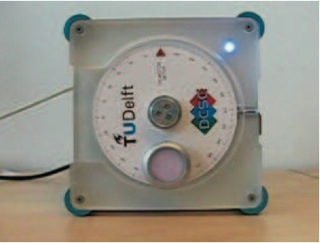
\includegraphics[width=.5\textwidth]{img/pendulum}
	\caption[Inverted pendulum setup]{Inverted pendulum setup.}
	\label{fig:PS-Inverted pendulum setup}
\end{figure}
The inverted pendulum was simulated in \textsc{Matlab} with a sampling time of \lsymb{$T_s$}{Sampling time}~$ = 0.03$~s. No noise was added to the system. The angle was wrapped to $\theta \in [-\pi, \pi]$ and the angular velocity was limited to $\omega \in [-10\pi, 10\pi]$. 
%A faster sampling time led to slower learning, a slower sampling time led to a worse resulting policy. 

\begin{table}[htbp]
	\centering
	\caption[Inverted pendulum: Parameter values]{Physical parameters of the inverted pendulum.}
	%                PAR.J = 0.005; PAR.K = 0.1; PAR.b = 0.01; PAR.m = 0.1; PAR.l = 0.1;
		\begin{tabular}{ll}
			\textbf{Symbol} & \textbf{Parameter} \\ \hline
			$m = 0.1 \textrm{ kg}$ & Pendulum mass \\
			$J = 1.91\cdot 10^{-4} \textrm{ kg/rad}^2$ & Pendulum inertia \\ %1.91E-4
			$g = 9.81 \textrm{ m/s}^2$ & Gravitational acceleration \\
			$l = 0.1 \textrm{ m}$ & Pendulum length \\
			$b = 0.01 \textrm{ kg/s}$ & Damping \\
			$K_R = 9.5 \Omega$ & Rotor resistance \\ %9.5
			$K_t = 5.36 \textrm{ Nm/A}$ & Torque constant %5.36E-4
		\end{tabular}
	\label{tab:PS-inverted pendulum parameters}
\end{table}


\subsection{Reward function}\label{sec:PS-learning problem reward}
The reward function can be implemented in two different ways. The first is a box-style reward. This reward originates from the idea that the goal state results in a reward and the other states in a penalty. As we are dealing with continuous states, we have to define a region around the goal that is considered close enough to the goal state. The box-style reward is defined as follows:
$$
	r(\theta,\omega) = 
		\left\{ \begin{array}{ll} 
%			+10, & \textrm{if } |\theta|<\delta_\theta \textrm{ and } |\omega|<\delta_\omega \\ 
			+10, & \textrm{if } |\theta|< \frac{10\pi}{180}\textrm{ rad} \textrm{ and } |\omega|< 0.3\textrm{ rad/s} \\  
			-1,  & \textrm{elsewhere} 
		\end{array} \right.
$$
%With $\delta_\theta$ and $\delta_\omega$ small values that define the region around zero that is considered to be the goal region. 
Where we have defined a region around zero that we consider as the goal region. With this type of reward, a learning trial is usually stopped when the goal region has been reached. 

Another option that is often used, is to use a smooth reward that gives a (negative) reward for every state-action pair:
$$
	\rho(\theta,\omega,u) = -\left[ \begin{array}{cc} \theta & \omega \end{array} \right]Q_\textrm{lq}\left[ \begin{array}{c} \theta \\ \omega \end{array} \right]- u R_\textrm{lq} u
$$
with $ Q_\textrm{lq} = \left[ \begin{array}{cc} 5 & 0 \\ 0 & 0.1 \end{array} \right]$ and $R_\textrm{lq} = 0.01$. This is a lqr-style reward and it will also drive the system to the goal state $[0, 0]^T$. Preliminary experiments showed that this reward resulted in a much faster learning speed than the box-reward, so we choose the smooth reward for the learning experiments. %\textcolor{red}{add: results box-style vs lqr-style}

A learning problem with lqr-rewards does not have an explicit goal state so learning trials are continuing. We have chosen to stop a trial whenever the goal region (as defined in the box-style reward) has been reached. This made no difference for the learning speed or the resulting policy. This can be explained by the fact that the system does not learn anything by moving around in the goal region. Adding a stopping criterion did reduce the simulation time significantly, since a large number of trials is stopped before maximum time for the episode ran out.

It has to be noted that although both reward structures have $[0, 0]^T$ as goal, the learning problem is not the same. The box-style reward results in a solution that gives the time-optimal policy to drive the system to the goal. The smooth reward results in a solution that is optimal with respect to the cost function $\rho$. This function also depends on the input signal $u$, so the optimal policy will try to limit the control signal as well as getting to the goal. The resulting policy will therefore not be time-optimal.



\subsection{Learning parameters}\label{sec:PS-learning problem parameters}
Tuning a \ac{RL} algorithm boils down to tuning three learning parameters: the discount factor $\gamma$, the learning rate $\alpha$ and the exploration rate $\epsilon$. The discount factor defines the solution to the learning problem and should therefore be fixed during the entire experiment. The learning rate influences how fast the value function is updated and thus how aggressively the agent learns. For noisy or stochastic experiments a high learning rate might lead to 'unlearning'. The exploration rate defines the percentage of random actions taken by the agent. The value may be constant or time-varying. The agent needs to explore in order to experience new state-action pairs and to avoid the learning of a sub-optimal policy. Unfortunately, no general rules for setting these parameters exist in the literature and the parameters have to be tuned empirically. 

We want to investigate the difference in performance between the \ac{RL} algorithms, we are not necessarily interested in the best performance for each case. Therefore, we did not try to fine-tune the parameters for every experiment, but set the tuning parameters to fixed values for all experiments. For \gsymb{$\gamma$}{Discount factor} and \gsymb{$\epsilon$}{Exploration rate} this seems reasonable. The first defines the solution and the second should have minor influence if multiple experiments are conducted. For the learning rate \gsymb{$\alpha$}{Learning rate} this might be questionable, because this factor immediately influences the update of the value function (\eqnref{eqn:RL-TDbasicQ}). The learning rate might have an optimal value for different experimental settings. For noisy environments or inaccurate models for instance, a low learning rate might be preferred. In noise-free environments with a very accurate model, a high learning rate might be used. Also different algorithms might have different optimal learning rates. 

The values of the learning parameters in a \ac{RL} experiment can be chosen freely and no rules for determining the optimal values exist. We chose the parameter values based on initial experiments and scientific intuition. The learning parameters were set as follows: 
$$
	\begin{aligned}
		\alpha &= 0.8 \\ 
		\gamma &= 0.98 \\
		\epsilon_{n_t} &= \max(0.1\cdot0.99^{n_t},0.001)
	\end{aligned}
$$
Where \lsymb{$n_t$}{Trial number} is the number of the current trial, so the exploration is decreased in every next trial, with a minimum of 0.001. A decreasing exploration rate led to faster learning than a fixed exploration rate and it led to a more 'smooth' learning curve. However, decreasing the exploration rate to zero led to occasionally finding a sub-optimal solution, so therefore the exploration was minimized to a small value. 


\subsection{Value function approximation: tile coding}\label{sec:PS-learning problem tile coding}
In the introduction of the value function in Section \ref{sec:RL-Value_functions}, it was assumed that a value is assigned to every state. This would lead to a tabular implementation of the value function in which every state has a value. As our state-space is continuous, this approach is impossible. Even discretizing the state-space into discrete bins, would still lead to a very large table. Therefore, we have to approximate the value function in some way.
\begin{figure}[htbp]
	\centering
		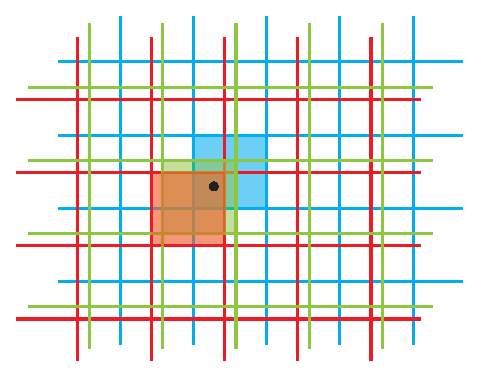
\includegraphics[width=.5\textwidth]{img/TileCoding}
%		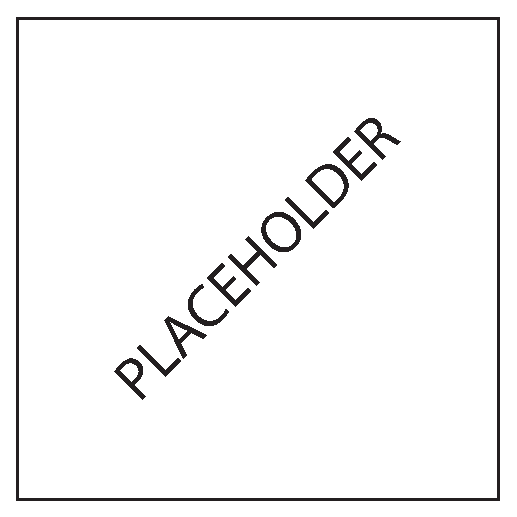
\includegraphics[width=.5\textwidth]{img/Placeholder}
	\caption[Tile Coding]{Schematic overview of Tile Coding. The black dot represents a continuous value. The colored grids represent three tilings and the continuous value is approximated by the shaded tiles.}
	\label{fig:PS-TileCoding}
\end{figure}

Tile coding (\figref{fig:PS-TileCoding}) is a commonly used way to approximate functions, because it is fast and easy to use. We used tile coding as a function approximator for the action-value function. We used 20 tilings of $30\times 30$ tiles each, which led to a final resolution of approximately $\Delta_\theta=0.01$ for the angle $\theta$ and $\Delta_\omega=0.1$ for the angular velocity $\omega$. These values are exact only if the tilings are displaced evenly with respect to each other. Because we use random displacements, the given resolutions are approximations. The tiles were initialized with a random value in the interval $[0,1]$. Again, we are not interested in achieving the best performance for every algorithm, but in creating a fixed experimental setting for all experiments. It is expected that the value-function will only influence the quality of the final policy and not the difference between the policies of different algorithms. 

In all our experiments the actions available to the controller form a discrete set, so only a limited number of actions can be used. This is a common approach in \ac{RL} because it limits the number of state-action pairs. Hence the action-value function only has to generalize over the states and not over the actions.
%The actions were used as discrete inputs so no generalization over the actions was used.

%We used SARSA to perform value updates. Some quick experiments with Q-learning were conducted but they did not lead to significantly different results.



\section{Implementation of Local Linear Regression} \label{sec:PS-LLR implementation}
In this chapter we use two model-learning methods: Dyna and \ac{PS}. We use \ac{LLR} as a model to generate state-transitions in Dyna and to determine lead-in states in \ac{PS}. Prediction intervals are used as a possible accuracy measure of the modeled output. The number of nearest neighbors used in the linear regression will be fixed to $K=5$, a value that is based on the results with the two-link manipulator in Section \ref{sec:LLR-two link manipulator}. 
 
Every experiment started with an empty memory, which was updated with experienced state-transitions during the learning process. A $k$d-tree structure was used to represent the memory as described in Section \ref{sec:LLR-kd-tree}. New samples were added to the $k$d-tree immediately. In order to maintain a balanced tree, we re-built the entire tree after a learning trial was completed. After the first 1000 samples, the tree is not re-built between trials anymore and samples are added to the existing tree only. The main reason for this is that the re-building consumes too much time for many samples. Furthermore, the sample-density will be sufficiently high so that new samples will not unbalance the tree severely. The 1000-sample border is chosen more or less arbitrarily, based on experience gained with the \ac{LLR} experiments of Chapter \ref{chap:Modeling}. 




\subsection{Prediction intervals} \label{sec:PS-Prediction intervals}
It is expected that the accuracy of the \ac{LLR} model improves as the number of memory samples increases and that it can vary over the state-space. Our approach to assess the quality of the model is to use prediction intervals around the modeled state-transition (see Section \ref{sec:LLR-prediction interval}). 

We will introduce a limit on the prediction interval which has to guarantee accurate model outputs. The calculated prediction interval \lsymb{$I_x$}{Calculated prediction interval for variable $x$} will be compared to an user imposed limit \lsymb{$\delta_x$}{Imposed prediction interval limit for variable $x$}. Whenever the prediction interval is larger than the maximum value in any dimension, the modeled state-transition is discarded. We can write this mathematically as follows:
%For a prediction interval $I_{x_i}$ of the $i$th state $x_i$, we define the maximum prediction interval as $\delta_{x_i}$.
$$
	\hat{y}_q = 
	 	 \left\{\begin{array}{ll}
		 	\textrm{LLR}(x_q)  &, \quad \textrm{if $I_{x_i} \leq \delta_{x_i}$ for $i=1,2,\hdots,k$} \\
		 	\textrm{no answer} &, \quad \textrm{if $I_{x_i} > \delta_{x_i}$ for $i=1,2,\hdots,k$}  
		 \end{array}\right.
$$
If the prediction interval is smaller than this limit, the state-transition will be considered accurate enough to be used. If the prediction interval is larger, the estimated state-transition will be discarded and not used for learning. In our experiments a discarded estimation was not replaced by a different (possibly accurate enough) estimation. This replicates the real-time situation in which only a limited amount of time is available to estimate state-transitions. Endlessly calculating state-transitions until an accurate estimate is found, is therefore not possible.

As discussed earlier, we have no clear idea how small the interval has to be in order to indicate that the estimation is good enough to be used for \ac{RL}. The main problem is that we have no quantity to relate the interval to. That is, if this quantity exists at all. It might also be true that very inaccurate predictions can be used as long as they meet certain restrictions. These restrictions may vary, depending on the learning problem.
%For instance an estimated state-transition that points in the right direction, but with very inaccurate velocity, might still be used without disturbing the learning process.

At this point, we choose for the prediction interval a limit that is related to the final resolution of the value function approximator. The idea behind this choice is based on the discriminating power of the model and the value function approximator. It seems reasonable that the optimal situation is a value function approximator and a model that have about the same 'resolution'. Increasing the accuracy of only one of them, would only have a minor effect as the overall accuracy would be limited by the other. Computational resources are therefore used optimally if the model and the value function have a similar accuracy.  

We will use two prediction interval limits. The first is based in the tile size in each tiling. As we divide each tiling into $30\times 30$ tiles, the tile size is $\frac{2\pi}{30}\times \frac{20\pi}{30}$. The corresponding prediction interval limit is $[\delta_\theta, \delta_\omega]=[0.2094, 2.094]$. The second limit is based on the final resolution of the tile coding approximator. As we used 20 tilings, the approximate final resolution is $[\delta_\theta, \delta_\omega]=[\Delta_\theta,\Delta_\omega]=[0.01, 0.1]$. \figref{fig:TCvsPredInt} shows the prediction interval limit for a certain modeled state-transition.
%\gsymb{$[\delta_\theta, \delta_\omega]$}{full prediction interval}
\begin{figure}[htbp]
	\centering
		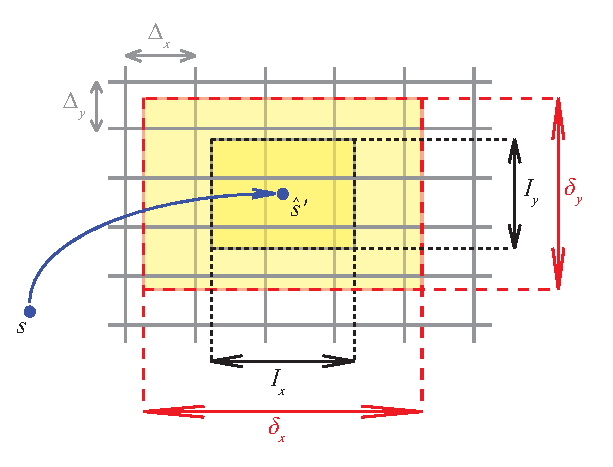
\includegraphics[width=.5\textwidth]{img/TCvsPREDINT}
	\caption[Prediction interval]{Limit of the prediction interval $[\delta_x,\delta_y]$ compared to the resolution of the value function $[\Delta_x,\Delta_y]$. The figure shows an estimated state-transition $s\rightarrow \hat{s}'$ with a prediction interval $[I_x,I_y]$. Because $[I_x,I_y]$ falls inside $[\delta_x,\delta_y]$, the corresponding prediction is considered accurate enough and is used for learning.}
	\label{fig:TCvsPredInt}
\end{figure}




\subsection{Lead-in states}\label{sec:PS-lead in states}

A crucial part in the \ac{PS} algorithm is determining lead-in states (Algorithm \ref{alg:PS}, line \ref{alg:PS_DetermineLeadInStates}). This process is not well described in literature. It is simply assumed that a model is available and that this model can be used to determine lead-in states. The type of model is not specified. We will describe our approach in this section.

First we have to note that we are actually not searching for lead-in states, but for lead-in state-action pairs. Consider the \ac{LLR} state-transition model \lsymb{$M$}{LLR model of the mapping $(s_t,a_t)\rightarrow s_{t+1}$} of the system. The state-transitions are then described by:
$$
	s_{t+1} = M \left[\begin{array}{c} s_t \\ a_t \\ 1 \end{array}\right]
$$
So we are actually searching for a state $s_t$ and an action $a_t$ that will lead to $s_{t+1}$. However, modeling the inverse mapping $s_{t+1}\rightarrow(s_t,a_t)$ would lead to two problems. First, one input could have several possible outputs (i.e., several state-action pairs $(s_t,a_t)$ can lead to $s_{t+1}$). So a unique model for this mapping does not exist. The second problem is that when this model would be used, we would obtain continuous values of $s_t$ and (more importantly) $a_t$. This is unwanted as we are assuming a discrete valued action-space.
%First, this mapping is ***Surjective?***. 

Our approach tries to solve these two issues. We consider the mapping $(s_{t+1},a_t)\rightarrow s_t$. This mapping can be modeled with an alternative model \lsymb{$\tilde{M}$}{LLR model of the mapping $(s_{t+1},a_t)\rightarrow s_t$} for which:
$$
	 s_t  = \tilde{M} \left[\begin{array}{c} s_{t+1} \\ a_t \\ 1 \end{array}\right]
$$
%Furthermore this mapping is ***injective??**, so the model is unique.
Because the action is now used as an input, we can choose a discrete value. The proposed mapping might seem counter intuitive, as the inputs are samples at different time steps. But this model should not be seen as an actual state-transition model. It should rather be regarded as a data mapping. We simply consider the sample $(s_{t+1}, a_t)$ as the input that leads to the output sample $s_t$. Note that the model $\tilde{M}$ is different from the state-transition model $M$. It is again obtained using \ac{LLR} techniques, but it requires a differently structured memory and a different input vector.

Now, for the target state $s$ the lead-in state-action pairs (\lsymb{$\bar{s}$}{Lead-in state to $s$},\lsymb{$\bar{a}$}{Lead-in action to $s$}) can be determined using the routine of Algorithm \ref{alg:lead-in states}. Note that every state, can have multiple lead-in states. Furthermore, we use the prediction interval limit (as described in Section \ref{sec:PS-Prediction intervals}) to possibly discard an estimated lead-in state. The notation $\bar{s}$ is used to denote a lead-in state to $s$. Subscripts containing time are usually avoided. 
\begin{algorithm}[ht]
	\caption{Lead-in states} \label{alg:lead-in states}
	\begin{algorithmic}[1]
		\State given $s$ 																\Comment{Target state}
		\For{ each $a \in \mathcal{A}$}
			\State $\tilde{M} \gets \textrm{LLR}(s,a)$ 		\Comment{Estimate LLR model $\tilde{M}$}
			\State $\hat{s} \gets \tilde{M}\left[\begin{array}{ccc} s & a & 1 \end{array}\right]^T$
			\If{ $I_{\hat{s}} \leq \delta_{s}$} 					\Comment{If prediction interval is sufficiently small}
				\State $(\bar{s},\bar{a})\gets(\hat{s},a)$ is a lead-in state	
			\EndIf		
		\EndFor
	\end{algorithmic}
\end{algorithm}


%\subsection{Look ahead Dyna (?)}
%\subsubsection{Estimating future states}






\section{Experimental results}\label{sec:PS-results}
We now present our experimental results. As explained in the beginning of this chapter, we used the same experimental setup and parameters for all experiments. All results shown in this section, are averages of 30 separate learning experiments. Every experiment consists of 1000 learning trials and every trial (or episode) consisted of a maximum of 100 time steps (equivalent to 3 seconds simulated time). This results in a maximum learning time of 50 minutes per experiment. Every experiment starts with a cleared \ac{LLR} memory and a randomly initialized value function.



\subsection{SARSA} \label{sec:PS-SARSA}
We have introduced the on-line, model-free algorithm SARSA in Section \ref{sec:RL-SARSA}. This is the most basic form of on-line learning. At every time step, one value function update is executed based on one real state-transition. SARSA can be considered as a 'benchmark' to which Dyna and \ac{PS} can be compared. In order for \ac{LLR} to be useful, the model-learning algorithms should perform better than a purely model-free algorithm. Furthermore, SARSA was used to get insight in the learning parameters and the optimal policy.

\figref{fig:PS-SARSA-learningcurve} shows the learning curve for the SARSA algorithm. The figure shows the reward per trial (a 3 second experiment), averaged over 30 separate experiments. We also show the standard deviation, minimum and maximum values in order to gain insight in the spread of the learning curve. The graph shows very rapid learning during the first 5~minutes. Thereafter, the policy strongly improves further until about 15~minutes of learning. The reason that the curve still fluctuates slightly thereafter is due to the exploration. 

Closer inspection of the experimental data, showed that it takes on average about 3~minutes to reach the goal for the first time. Although the maximum duration of a learning experiment is 50~minutes, the added stopping criterion leads to an average experiment length of 25.4~minutes. During this period the SARSA algorithm used on average $5.1\cdot 10^4$ real experiences to learn. 
\begin{figure}[htbp]
	\centering
	\subfigure[{SARSA learning curve}]{ 
		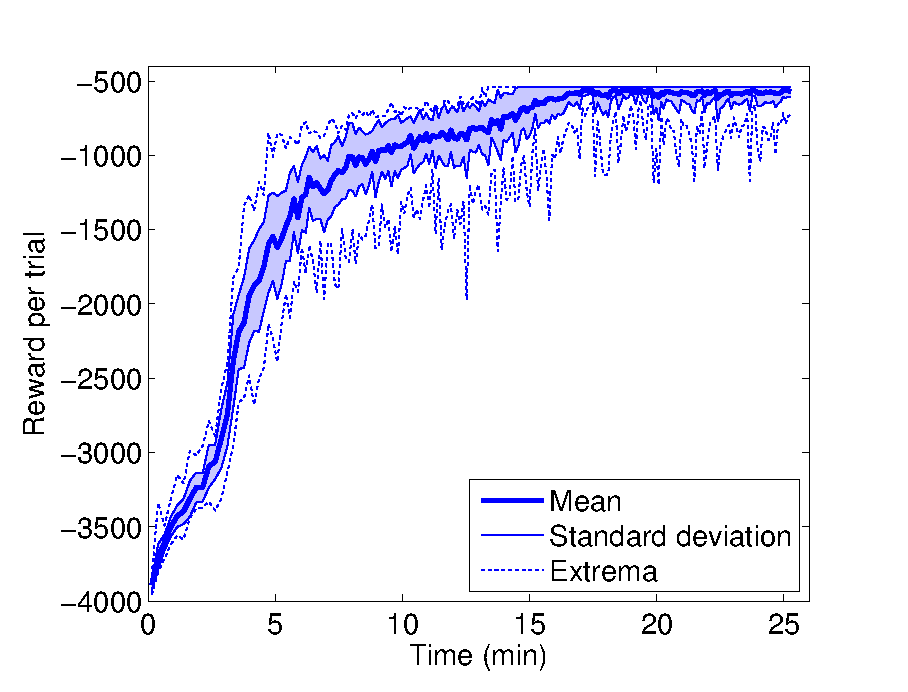
\includegraphics[width=.45\textwidth]{figures/PS-SARSA-learningcurve}	
	\label{fig:PS-SARSA-learningcurve}
	}
	\subfigure[{SARSA compared to Q-learning}]{ 
		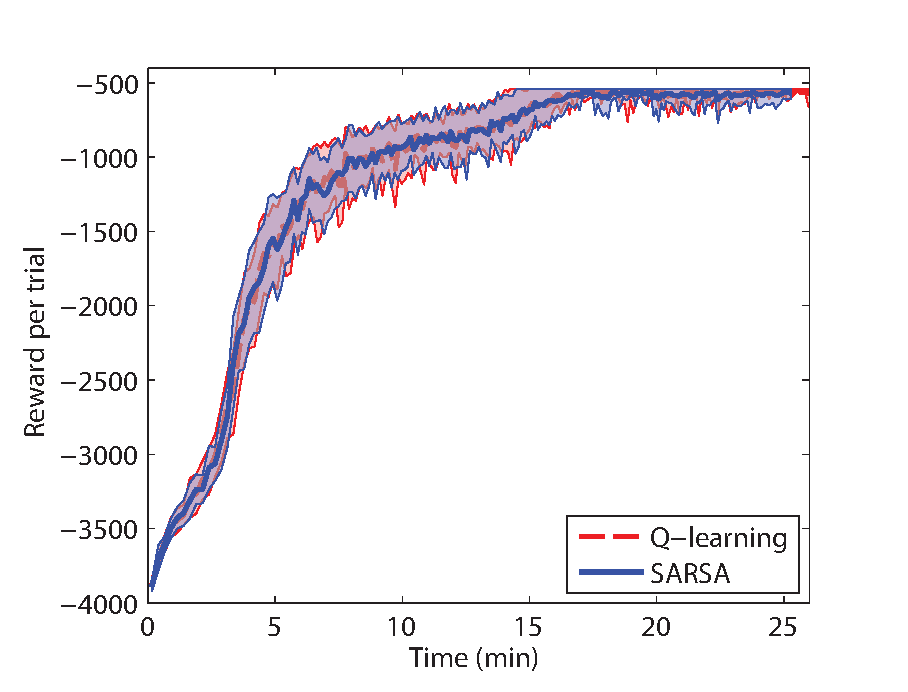
\includegraphics[width=.45\textwidth]{figures/PS-SARSAvsQlearning}	
	\label{fig:PS-SARSAvsQlearning}
	}
%	\subfigure[{Optimal policy}]{ 
%		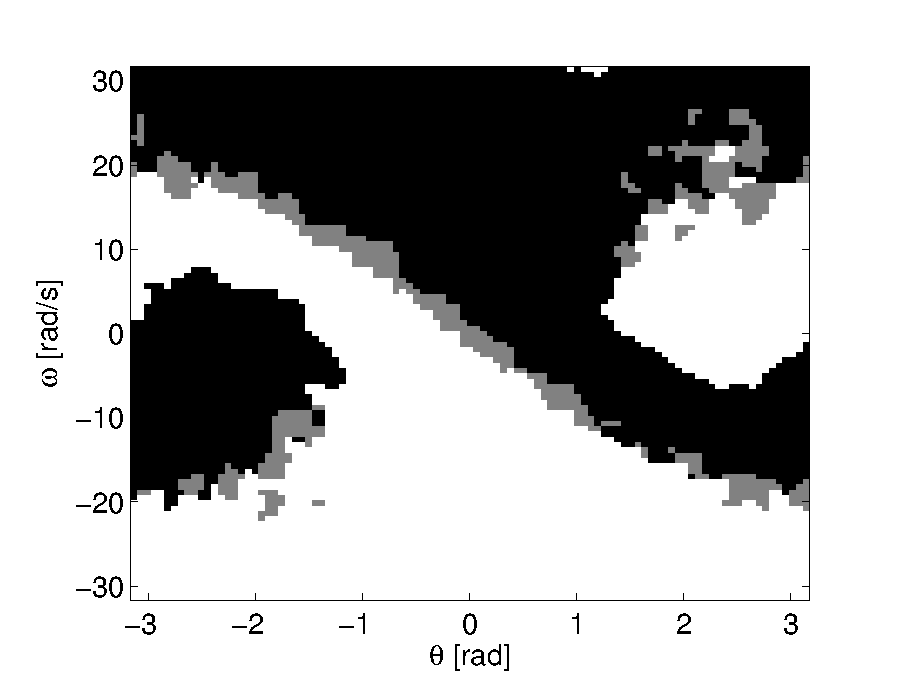
\includegraphics[width=.45\textwidth]{figures/PS-invpend_optimalpolicy}	
%	\label{fig:PS-optimal policy}
%	}
	\caption[Inverted pendulum: Model-free learning]{Learning curves of model-free learning applied on the inverted pendulum simulation. \subref{fig:PS-SARSA-learningcurve} shows the reward per trial during an experiment consisting of 1000 trials using SARSA as learning algorithm. The graph shows the average value (solid line), the standard deviation (shaded area) and the extreme values (dashed lines) of 30 separate experiments. \subref{fig:PS-SARSAvsQlearning} compares SARSA and Q-learning.}
	\label{fig:PS-SARSAlearningCurve}
\end{figure}

%In order to get insight in how the optimal policy looks, we executed a SARSA experiment for 10000 trials. \figref{fig:PS-optimal policy} shows the obtained %policy after 10000 trials. We use this policy as (an approximation of) the optimal policy for this problem.

We could also have used the model-free algorithm Q-learning (Section \ref{sec:RL-Q_learning}) instead of SARSA. Preliminary experiments with the two algorithms (\figref{fig:PS-SARSAvsQlearning}) showed no significant difference in learning speed between the two algorithms. When combined with function approximators, SARSA has better convergence properties than Q-learning \cite{Gordon:95}, so we will use SARSA to update the value function in the remaining of this chapter.
%\begin{figure}[htbp]
%	\centering
%		\includegraphics[width=.7\textwidth]{figures/PS-SARSAvsQlearning}
%	\caption[Inverted pendulum: SARSA compared to Q-learning]{Comparison of the learning curves using SARSA and Q-learning for the inverted pendulum. The graph compares the model-free SARSA (solid line) and Q-learning (dashed line) algorithms.}
%	\label{fig:PS-SARSAvsQlearning}
%\end{figure}

The learning curves presented in the chapter show the reward per trial. The results show that the agent learns a policy along the trajectory towards the goal. However, this does not necessarily mean that the policy has converged for the entire state-space. In Appendix \ref{app:Policies} we show the final policy for all learning algorithms and compares them to the optimal policy.

\subsection{Dyna} \label{sec:PS-Dyna}
We now add the \ac{LLR} model to the learning process and combine it with the Dyna algorithm (see Section \ref{sec:RL-Dyna}). The modeled state-action pairs are chosen randomly throughout the state-space. The \ac{LLR} model is built and used as described in Section \ref{sec:PS-LLR implementation}. Initially the memory is empty and every new experience is immediately added to it. We generated $N_m = 3$ state-transitions every time step. Prediction intervals of the \ac{LLR} model are used to possibly discard an estimate if it exceeds a given limit (see Section \ref{sec:PS-Prediction intervals}).

We compared several values for the maximum prediction interval. Due to the limit on the prediction interval, not all modeled state-transitions are used by the learning agent. \tabref{tab:PS-dyna updates} summarizes the number of iterations and value-function updates of the different settings. It is clear that setting this limit tighter, leads to more discarded model-outputs. In the case of a very tight limit of $[0.001,0.01]$, 86~\% of the modeled outputs get discarded. In the case of a less tight limit of $[0.2094,2.0944]$, only 37\% get discarded. 

\begin{table}[htbp]
	\centering
	\caption[Inverted pendulum: Learning results]{Results of the learning experiments on the inverted pendulum using different algorithms. The results are averages of 30 experiments, consisting of 1000 trials, generating $N_m=3$ modeled state-transitions per time interval. 'Iterations' are the total number of simulated time steps, 'Updates' are the total number of value-function updates (model-free and model-based), 'Ratio' is the ratio of model-free updates to model-based updates.}
		\begin{tabular}{l|llll}
			\textbf{Algorithm} & $[\delta_\theta,\delta_\omega]$ & \textbf{Iterations} $[10^4]$  & \textbf{Updates} [$10^4$]& \textbf{Ratio}  \\ 
			\hline\hline
			SARSA 								& -										&   4.95  &   4.95  & 1:0			\\  
			Q-learning 						&	-										&   5.11  &   5.11  & 1:0 		\\   
			\hline 
			Dyna 						  		& $[0.001, 0.01]$ 		&   4.94  &   6.98  & 1:0.41  \\ 
			(\ac{LLR} model)	 		& $[0.01, 0.1]$				&   4.22  &   8.73  & 1:1.07	\\ 
			 											& $[0.2094, 2.0944]$	&   3.97  &  11.93  & 1:2.01  \\ 
			 											& $[\infty,\infty]$		&   4.17  &  16.69  & 1:3     \\	
			\hline
			Dyna (exact model)		& -										&   3.65  &  14.61  & 1:3     \\
			\hline			 
			\acl{PS} 							& $[0.001, 0.01]$			&   4.77  &   9.30  & 1:0.95  \\ 
			(\ac{LLR} model) 			& $[0.01, 0.1]$				&   4.76  &  13.93  & 1:1.93  \\
			 											& $[0.2094, 2.0944]$	&   4.38  &  16.59  & 1:2.79  \\ 
			 											& $[\infty, \infty]$	&   6.31  &  25.24  & 1:3     
			\\ \hline
			Look Ahead Dyna				& $[0.001, 0.01]$			&   4.71  &  12.61  & 1:1.68	\\
			(\ac{LLR} model)			& $[0.01, 0.1]$				&   4.42  &  15.38  & 1:2.48	\\
														& $[0.2094, 2.0944]$	&   4.14  &  16.01  & 1:2.87 	\\
														& $[\infty, \infty]$	&   4.42  &  17.67  & 1:3      			 												
		\end{tabular}
	\label{tab:PS-dyna updates}
\end{table}
% Computation times (1000 trials/3000 seconds/50 minutes, Nm = 3, dualcore intel):
% SARSA: 	80 seconds/1.3 minutes	 --> 24 min experiment (~18x realtime)
% DYNA: 	170 seconds/~3 minutes   --> 20 min experiment (~6x realtime)
% LA: 		150	seconds/~2.5 minutes --> 20 min experiment (~8x realtime)
% PS: 		600 seconds/10 minutes   --> 22 min experiment (~2x realtime)

\begin{table}[htbp]
	\centering
	\caption[Computation times of the learning algorithms]{Computation time needed to perform all calculations in a single time step of the different learning algorithms for $N_m=3$. The table shows the mean time and the maximum time needed (during the entire experiment). The results were obtained using a 3~GHz desktop computer. Notice that the sampling time of the simulation is $T_s = 30\cdot 10^{-3}$~s.}
		\begin{tabular}{l|ll}
			\textbf{Algorithm} & \textbf{Mean [$10^{-3}$~s]} & \textbf{Max [$10^{-3}$~s]} \\ 
			\hline\hline
			SARSA & 1.01 & 1.94 \\
			Dyna  & 2.75 & 5.97 \\
			Prioritized Sweeping & 4.65 & 8.51 \\
			Look Ahead Dyna & 2.38 & 4.71 
		\end{tabular}
	\label{tab:PS-computation times}
\end{table}

%SARSA|   min: 0.00088196    max: 0.0019448    mean: 0.0010612
%DYNA|   min: 0.0019265    max: 0.0059695    mean: 0.0027438
%PS|   min: 0.00094839    max: 0.0085139    mean: 0.0046493
%LA|   min: 0.0010011    max: 0.0047052    mean: 0.0023847

We now continue with a closer inspection of the performance of the different \ac{LLR} settings. \figref{fig:PS-DYNA} shows the reward per trial during the learning process for the different settings. We notice that a large limit on the prediction interval leads to faster learning. The learning speed differs particularly in the first five minutes of the learning process. Furthermore, we notice that the spread in the learning curves increases with decreasing prediction interval limits. For very tight limits, the spread is very similar to the SARSA result. Using many uncertain outputs is preferred as this results in a smaller spread of the learning curve. This might be counter-intuitive as it is expected that highly inaccurate state-transitions lead to faulty value-function updates. However, this effect is apparently counteracted by the high number of value-function updates.

\begin{figure}[htbp]
	\centering
	\subfigure[{$[\delta_\theta,\delta_\omega]=[0.001,0.01]$}]{ 
		\includegraphics[width=.45\textwidth]{Figures/PS-DYNA1-learningcurve}
	\label{fig:PS-DYNA1-learningcurve}
	}
	\subfigure[{$[\delta_\theta,\delta_\omega]=[0.01,0.1]$}]{ 
		\includegraphics[width=.45\textwidth]{Figures/PS-DYNA2-learningcurve}
	\label{fig:PS-DYNA2-learningcurve}
	}\\
	\subfigure[{$[\delta_\theta,\delta_\omega]=[0.2094,2.0944]$}]{ 
		\includegraphics[width=.45\textwidth]{Figures/PS-DYNA3-learningcurve}
	\label{fig:PS-DYNA3-learningcurve}
	}
	\subfigure[{$[\delta_\theta,\delta_\omega]=[\infty,\infty]$}]{ 
		\includegraphics[width=.45\textwidth]{Figures/PS-DYNA4-learningcurve}
	\label{fig:PS-DYNA4-learningcurve}
	}
	\caption[Inverted pendulum: Dyna]{Learning curves of the Dyna algorithm applied on the inverted pendulum. \subref{fig:PS-DYNA1-learningcurve}, \subref{fig:PS-DYNA2-learningcurve}, \subref{fig:PS-DYNA3-learningcurve} and \subref{fig:PS-DYNA4-learningcurve} show the Dyna algorithm using \ac{LLR} with increasing prediction interval limits.}
	\label{fig:PS-DYNA}
\end{figure}

\figref{fig:PS-DYNA_hLLR} shows another effect of the limit on the prediction interval. The figure shows the positions in state-space for which a modeled state-transition was generated and not discarded. It is clear that the sample density and the prediction interval are related. For a very tight limit (\figref{fig:PS-DYNA1_hLLR}), only in the vicinity of the optimal trajectory enough samples are available for an estimated state-transition that is accurate enough. When the limit is stretched (\figref{fig:PS-DYNA2_hLLR}-\ref{fig:PS-DYNA3_hLLR}), so is the region in which the model is considered to be accurate enough. If no limit is imposed (\figref{fig:PS-DYNA4_hLLR}), the modeled state-transitions in the entire state-space are used.

\begin{figure}[htbp]
	\centering
	\subfigure[{$[\delta_\theta,\delta_\omega]=[0.001,0.01]$}]{
		\includegraphics[width=.45\textwidth]{Figures/PS-DYNA1_hLLR}
	\label{fig:PS-DYNA1_hLLR}
	}
	\subfigure[{$[\delta_\theta,\delta_\omega]=[0.01,0.1]$}]{ 
		\includegraphics[width=.45\textwidth]{Figures/PS-DYNA2_hLLR}
	\label{fig:PS-DYNA2_hLLR}
	}\\
	\subfigure[{$[\delta_\theta,\delta_\omega]=[0.2094,2.0944]$}]{
		\includegraphics[width=.45\textwidth]{Figures/PS-DYNA3_hLLR}
	\label{fig:PS-DYNA3_hLLR}
	}
	\subfigure[{$[\delta_\theta,\delta_\omega]=[\infty,\infty]$}]{
		\includegraphics[width=.45\textwidth]{Figures/PS-DYNA4_hLLR}
	\label{fig:PS-DYNA4_hLLR}
	} 
	\caption[Inverted pendulum: Distribution of model-generated experience using Dyna]{Distribution of states for which a state-transition was generated using the \ac{LLR} model in the Dyna setting. The figures only show the states for which the prediction interval was smaller than the given limit. The color indicates the number of times a state-transition was generated in a certain area.}
	\label{fig:PS-DYNA_hLLR}
\end{figure}

\figref{fig:PS-SARSAvsDYNA} shows the average learning curve of the Dyna algorithms compared to model-free SARSA learning. We conclude that using model-generated experience in the learning process increases the learning speed. Increasing the limit on the prediction interval leads to more state-transition available to the agent. The graph shows that this leads to faster learning. The inaccuracy of these state-transition does not seem to influence the learning process negatively. 

Although all algorithms converge, the final reward per trial is slightly higher for SARSA. This indicates that the final trajectory towards the goal for SARSA is slightly better, with respect to the reward function, than for Dyna. So we can conclude that adding state-transitions generated by the \ac{LLR} model only has a minor negative effect on the resulting trajectory, even if highly inaccurate state-transitions are being used. Apparently, the number of real experience and accurate modeled state-transitions are high enough to counteract the negative effect of the inaccurate model outputs. Furthermore, it can be expected that the inaccurate state-transitions can mainly be found in rarely visited parts of the state-space (see also \figref{fig:PS-DYNA_hLLR}). These regions have a limited effect on the trajectory towards to goal.

A question posed earlier was: is it more useful to use many inaccurate model-outputs or to use a limited number of very accurate outputs? If we regard the prediction interval as a good indication, we can answer this question by comparing the values in \tabref{tab:PS-dyna updates} with the learning curves in \figref{fig:PS-SARSAvsDYNA}. It can be concluded that the number of value-function updates is dominant over the quality of the state-transitions. In other words, the optimal setting for Dyna in this test setup is to use as many model-outputs as possible by setting the limit on the prediction interval to a high value.
\begin{figure}[htbp]
	\centering
		\includegraphics[width=.7\textwidth]{figures/PS-SARSAvsDYNA}
	\caption[Inverted pendulum: Dyna compared to SARSA]{Comparison of the learning curves using SARSA and Dyna for the inverted pendulum for several values of the prediction interval limit $[\delta_\theta,\delta_\omega]$.}
	\label{fig:PS-SARSAvsDYNA}
\end{figure}

From the results in this section we can conclude that generating state-transitions using the \ac{LLR} model can increase the learning speed compared to model-free SARSA. We have seen that limiting the prediction interval influences the learning speed. However, we do not have an indication of the accuracy of the modeled state-transitions. For this, we need the true state-transitions. These can be obtained from \eqnref{eqn:PS-inverted pendulum}. We have applied Dyna using the exact model. This represents the optimal Dyna setting: a perfect model of the system throughout the state-space. We define the prediction interval of the exact model as $I = [0, 0]$. In \figref{fig:PS-DYNA4vsDYNANL} we compared the exact model to the optimal \ac{LLR} model. 

We notice that the curves are very close together. This means that the \ac{LLR} model does not disturb the learning process compared to the true model. In the first minutes of learning, both methods perform almost equally. This is surprising, as it is expected that early in the learning process the \ac{LLR} is not very accurate yet because of the low number of memory samples. Apparently, possibly inaccurate model outputs are still suitable for learning in the beginning. In the remaining of the learning process, the exact model has a very slight advantage over the \ac{LLR} model. 

The inaccuracy of the \ac{LLR} model is best seen in the later stages of the learning process. Although both learning curves converge to more or less the same value, the standard deviation of the exact model is about half the size of the \ac{LLR} model. This is caused by the inaccurate model outputs that are used by the Dyna algorithm using the \ac{LLR} model. 

\begin{figure}[htbp]
	\centering
		\includegraphics[width=.7\textwidth]{figures/PS-DYNA3vsDYNANL}
	\caption[Inverted pendulum: Dyna, \acs{LLR} model compared to exact model]{Comparison of the learning curves using Dyna with the \ac{LLR} model and the exact model on the inverted pendulum. We used $[\delta_\theta,\delta_\omega]=[0.2094, 2.0944]$ for the prediction interval limit of the \ac{LLR} model, which is the optimal setting.}
	\label{fig:PS-DYNA4vsDYNANL}
\end{figure}

In Section \ref{sec:LLR-kd-tree} we explained how we used a $k$d-tree to represent the memory in order to increase the computational speed of the \ac{LLR} model. Although in these simulation experiments the computation time is not limited, in real-time experiments all the calculations need to be performed within the sampling interval. The sampling time of the simulation was set to $T_s = 0.03$~s. Table \ref{tab:PS-computation times} shows the time needed by the learning algorithms in every sampling interval to perform all the calculations. The exact computation times will depend on the hardware and software used, so the values should be regarded only as indicative.

\subsection{Prioritized Sweeping}
We continue with \ac{PS} as a learning algorithm. Our \ac{PS} implementation will combine \ac{PS} (Algorithm \ref{alg:Dyna}) with \ac{LLR}. The lead-in states will be calculated as described in Section \ref{sec:PS-lead in states} and we set limits on the prediction interval in the same way as we did for Dyna. 
%The prediction interval limits are also used in determining the lead-in states (Algorithm \ref{alg:lead in states}).

First we investigate the influence of the prediction interval limit. \figref{fig:PS-PS} shows the learning curves for the \ac{PS} algorithm for several limits. We notice that the results differ in many aspects from the Dyna results. First we notice that for \ac{PS} we find an optimal value for the prediction interval limit. Out of the four intervals we have compared, $[\delta_\theta,\delta_\omega]=[0.2094,2.0944]$ performs best. This limit performs best both in terms of learning speed and in the variance of the learning curves. The other interval limits lead to worse results, with the worst result for $[\infty, \infty]$. For this large limit, the learning curve shows very slow learning, a large spread and no convergence to the optimal policy. Apparently the number of inaccurate state-transitions is so large that they severely disturb the learning process.

\begin{figure}[htbp]
	\centering
	\subfigure[{$[\delta_\theta,\delta_\omega]=[0.001,0.01]$}]{
		\includegraphics[width=.45\textwidth]{Figures/PS-PS1-learningcurve}
	\label{fig:PS-PS1-learningcurve}
	}
	\subfigure[{$[\delta_\theta,\delta_\omega]=[0.01,0.1]$}]{ % $0.001, 0.01$]{ %
		\includegraphics[width=.45\textwidth]{Figures/PS-PS2-learningcurve}
	\label{fig:PS-PS2-learningcurve}
	}\\
	\subfigure[{$[\delta_\theta,\delta_\omega]=[0.2094,2.0944]$}]{
		\includegraphics[width=.45\textwidth]{Figures/PS-PS3-learningcurve}
	\label{fig:PS-PS3-learningcurve}
	}
	\subfigure[{$[\delta_\theta,\delta_\omega]=[\infty,\infty]$}]{
		\includegraphics[width=.45\textwidth]{Figures/PS-PS4-learningcurve}
	\label{fig:PS-PS4-learningcurve}
	} 
	\caption[Inverted pendulum: \acs{PS}]{Learning curves of \ac{PS} applied on the inverted pendulum problem. \subref{fig:PS-PS1-learningcurve}, \subref{fig:PS-PS2-learningcurve}, \subref{fig:PS-PS3-learningcurve} and \subref{fig:PS-PS4-learningcurve} show the \ac{PS} algorithm using \ac{LLR} with increasing prediction interval limits.}
	\label{fig:PS-PS}
\end{figure}

\begin{figure}[htbp]
	\centering
	\subfigure[\ac{PS} learning curves]{ 
		\includegraphics[width=.45\textwidth]{Figures/PS-PSlearningcurves}
	\label{fig:PS-PSlearningcurves}
	}	
	\subfigure[Comparison of \ac{PS}, Dyna and SARSA]{
		\includegraphics[width=.45\textwidth]{Figures/PS-PSvsDYNAvsSARSA}
	\label{fig:PS-PSvsDYNAvsSARSA}
	}
	\caption[Inverted pendulum: \acs{PS} compared to Dyna and SARSA]{Learning curves for \ac{PS} algorithm applied on the inverted pendulum setup. \subref{fig:PS-PSlearningcurves} compares \ac{PS} using four different values for the prediction interval limit, \subref{fig:PS-PSvsDYNAvsSARSA} compares the optimal settings of \ac{PS}, Dyna and SARSA.}
	\label{fig:PS-PScompared}
\end{figure}

\figref{fig:PS-PSlearningcurves} compares the learning speed of the different \ac{PS} settings. It is clear that \ac{PS} needs a limit on the prediction interval. The setting with no limit leads to a very slow learning speed, even slower than SARSA. In the 1000-trial experiment, this setting did not converge to a solution. Also the setting with very tight bounds does not perform well. This setting leads to a learning speed that is similar to model-free SARSA.

%\begin{figure}[htbp]
%	\centering
%		\includegraphics[width=.7\textwidth]{figures/PS-PSlearningcurves}
%	\caption[Inverted pendulum: Prioritized Sweeping compared to SARSA]{Learning curves of \ac{PS} compared to SARSA for the inverted pendulum. Several values for the prediction interval limit $[\delta_\theta,\delta_\omega]$ are shown.}
%	\label{fig:PS-PSlearningcurves}
%\end{figure}

%\begin{figure}[htbp]
%	\centering
%		\includegraphics[width=.7\textwidth]{figures/PS-PSvsDynavsSarsa}
%	\caption[Inverted pendulum: Prioritized Sweeping, Dyna and SARSA compared]{Learning curves of SARSA, Dyna and \ac{PS}. For all algorithms the setting with the best result is shown. Dyna: $[0.2094,2.0944]$, \ac{PS}: $[0.2094,2.0944]$.}
%	\label{fig:PS-PSvsDynavsSarsa}
%\end{figure}

It is also interesting to look at the number of updates used by the best ($[0.2094,2.0944]$) and worst ($[\infty,\infty]$) \ac{PS} case (\tabref{tab:PS-dyna updates}). We notice that the ratio's of the optimal (1:2.79) and worst (1:3) setting are actually very close together. Hence, the number of discarded state-transitions in the optimal case is not much higher. But apparently, the small amount of inaccurate estimates is enough to severely influence the learning process negatively.

If we compare the ratio of the model-generated versus model-free state-transitions of Dyna and \ac{PS} we notice that this ratio is higher in \ac{PS}. The priority queue leads to generated state-transitions that are close to the trajectory to the goal state. In these areas the number of memory samples is high and therefore accurate predictions can be made. Therefore, less model outputs are rejected than in the Dyna case where state-transitions are generated randomly in the entire state-space.

The best performance is obtained with the interval limit $[0.2094,2.0944]$. \figref{fig:PS-PSvsDYNAvsSARSA} shows the learning curve of the optimal \ac{PS} algorithm compared to Dyna and SARSA. The figure shows that the \ac{PS} algorithm learns faster than both Dyna and SARSA. Especially in the first minutes of learning, the prioritized updates of the value-function lead to faster learning than Dyna.



%\begin{figure}[htbp]
%	\centering
%	\subfigure[{$[\delta_\theta,\delta_\omega]=[0.001,0.01]$}]{
%		\includegraphics[width=.45\textwidth]{Figures/PS-PS1_hLLR}
%	\label{fig:PS-PS1_hLLR}
%	}
%	\subfigure[{$[\delta_\theta,\delta_\omega]=[0.01,0.1]$}]{ 
%		\includegraphics[width=.45\textwidth]{Figures/PS-PS2_hLLR}
%	\label{fig:PS-PS2_hLLR}
%	}\\
%	\subfigure[{$[\delta_\theta,\delta_\omega]=[0.2094,2.0944]$}]{
%		\includegraphics[width=.45\textwidth]{Figures/PS-PS3_hLLR}
%	\label{fig:PS-PS3_hLLR}
%	}
%	\subfigure[{$[\delta_\theta,\delta_\omega]=[\infty,\infty]$}]{
%		\includegraphics[width=.45\textwidth]{Figures/PS-PS4_hLLR}
%	\label{fig:PS-PS4_hLLR}
%	} 
%	\caption[Inverted pendulum: Sample distribution]{Distribution of states for which a modeled state-transitions was generated in the Dyna setting. The figures only show the states for which the prediction interval was smaller than the given limit.}
%	\label{fig:PS-PS_hLLR}
%\end{figure}

\subsection{Look Ahead Dyna} 
Let us consider \ac{PS} simply as a method to generate specific model-based experiences instead of random experiences. We then might introduce other methods to generate useful state-transitions - not necessarily according to a priority measure. A possible method could be to use the model to 'look ahead' from the current state. Imagine a state-transition $s \rightarrow s'$. We then use the model to estimate $s' \rightarrow s''$ for all actions. The only issue is that the next state $s'$ is not yet known when the model-based experiences are generated. Therefore, the next state has also got to be estimated. Algorithm \ref{alg:Look Ahead Dyna} shows this method, which we will call \ac{LA Dyna}.

The Look Ahead approach partly originates from the earlier \ac{LLR} experiments on the two-link manipulator and robot Leo (Sections \ref{sec:LLR-two link manipulator} and \ref{sec:LLR-robot leo}). In those settings we used the \ac{LLR} model to estimate a state-transition in the vicinity of the current state. \ac{LLR} was able to generate very accurate estimates of complex systems using only a small number of experiences. We use this ability to model future state-transitions in this 'Look Ahead' setting.
\begin{algorithm}[ht]
	\caption{Look Ahead Dyna} \label{alg:Look Ahead Dyna}
	\begin{algorithmic}[1]
		\State Initialize $Q(s,a)$ randomly
		\For{ each time step $t$}
			\State $s\gets \textrm{ Current state}$
			\State Select $a$ using policy
			\State Execute $a$ 
			\State Estimate $\hat{s}' \gets \textrm{LLR }(s,a)$
			\For{each $a\in \mathcal{A}$}
				\State $(\hat{s}'',r) \gets Model(\hat{s}',a)$
				\State $\delta \gets r + \gamma Q(\hat{s}'',a') - Q(\hat{s}',a)$
				\State $Q(s',a) \gets Q(s',a) + \alpha \delta$
			\EndFor
			\State Observe $s'$, $r$
			\State $\delta \gets r + \gamma Q(s',a') - Q(s,a)$
			\State $Q(s,a) \gets Q(s,a) + \alpha \delta$
		\EndFor
	\end{algorithmic}
\end{algorithm}


\subsubsection{Results}
We applied \ac{LA Dyna} on the inverted pendulum simulation. \figref{fig:PS-LA} shows the resulting learning curves for different values of the prediction interval limit. The prediction interval is needed in the \ac{LA Dyna} algorithm. No limit on the prediction interval leads to severe 'unlearning', as can be seen in \figref{fig:PS-LA4-learningcurve}. This effect was also seen in the case of the \ac{PS} algorithm. Clearly, when the value function updates are close to the optimal trajectory, the estimated state-transitions need to be accurate. 

\begin{figure}[htbp]
	\centering
	\subfigure[{$[\delta_\theta,\delta_\omega]=[0.001,0.01]$}]{ 
		\includegraphics[width=.45\textwidth]{Figures/PS-LA1-learningcurve}
	\label{fig:PS-LA1-learningcurve}
	}
	\subfigure[{$[\delta_\theta,\delta_\omega]=[0.01,0.1]$}]{ 
		\includegraphics[width=.45\textwidth]{Figures/PS-LA2-learningcurve}
	\label{fig:PS-LA2-learningcurve}
	}\\
	\subfigure[{$[\delta_\theta,\delta_\omega]=[0.2094,2.0944]$}]{ 
		\includegraphics[width=.45\textwidth]{Figures/PS-LA3-learningcurve}
	\label{fig:PS-LA3-learningcurve}
	}
	\subfigure[{$[\delta_\theta,\delta_\omega]=[\infty,\infty]$}]{ 
		\includegraphics[width=.45\textwidth]{Figures/PS-LA4-learningcurve}
	\label{fig:PS-LA4-learningcurve}
	}
	\caption[Inverted pendulum: \acs{LA Dyna}]{Learning curves of the \ac{LA Dyna} algorithm applied on the inverted pendulum. \subref{fig:PS-LA1-learningcurve}, \subref{fig:PS-LA2-learningcurve}, \subref{fig:PS-LA3-learningcurve} and \subref{fig:PS-LA4-learningcurve} show the \ac{LA Dyna} algorithm using \ac{LLR} with increasing prediction interval limits.}
	\label{fig:PS-LA}
\end{figure}

\begin{figure}[htbp]
	\centering
	\subfigure[\ac{LA Dyna} learning curves]{ 
		\includegraphics[width=.45\textwidth]{Figures/PS-LAlearningcurves}
	\label{fig:PS-LAlearningcurves}
	}	
	\subfigure[Comparison of \ac{LA Dyna}, \ac{PS}, Dyna and SARSA]{
		\includegraphics[width=.45\textwidth]{Figures/PS-LAvsPSvsDYNAvsSARSA}
	\label{fig:PS-LAvsPSvsDYNAvsSARSA}
	}
	\caption[Inverted pendulum: \acs{LA Dyna} compared to \acs{PS}, Dyna and SARSA]{Learning curves for the \ac{LA Dyna} algorithm applied on the the inverted pendulum setup. \subref{fig:PS-LAlearningcurves} compares \ac{LA Dyna} using four different values for the prediction interval limit, \subref{fig:PS-LAvsPSvsDYNAvsSARSA} compares the optimal settings of the four different learning algorithms.}
	\label{fig:PS-LAcompared}
\end{figure}

The optimal value for the prediction interval limit is $[0.2094,2.0944]$, which is equal to the optimal value for Dyna and \ac{PS}.

In \figref{fig:PS-LAvsPSvsDYNAvsSARSA} we compared \ac{LA Dyna} to SARSA, Dyna and \ac{PS}. It can be seen that \ac{LA Dyna} learns faster than the other algorithms. The faster learning can mainly be seen in the first part of the learning process. The \ac{LA Dyna} algorithm also results in less spread in the learning speed. The variance of the \ac{LA Dyna} is about half of the variance of the other algorithms.

\figref{fig:PS-LA_hLLR} shows the distribution of the model-generated state-transitions. As expected, the state-transitions are located primarily in the neighborhood of the trajectories followed by the system. A possible reason for the fast learning of \ac{LA Dyna} could be that the majority of the value function updates are very close to the current state of the real system.

\begin{figure}[htbp]
	\centering
	\subfigure[{$[\delta_\theta,\delta_\omega]=[0.001,0.01]$}]{
		\includegraphics[width=.45\textwidth]{Figures/PS-LA1_hLLR}
	\label{fig:PS-LA1_hLLR}
	}
	\subfigure[{$[\delta_\theta,\delta_\omega]=[0.01,0.1]$}]{ 
		\includegraphics[width=.45\textwidth]{Figures/PS-LA2_hLLR}
	\label{fig:PS-LA2_hLLR}
	}\\
	\subfigure[{$[\delta_\theta,\delta_\omega]=[0.2094,2.0944]$}]{
		\includegraphics[width=.45\textwidth]{Figures/PS-LA3_hLLR}
	\label{fig:PS-LA3_hLLR}
	}
	\subfigure[{$[\delta_\theta,\delta_\omega]=[\infty,\infty]$}]{
		\includegraphics[width=.45\textwidth]{Figures/PS-LA4_hLLR}
	\label{fig:PS-LA4_hLLR}
	} 
	\caption[Inverted pendulum: Distribution of model-generated experience using \acs{LA Dyna}]{Distribution of states for which a state-transition was generated using the \ac{LLR} model in the \ac{LA Dyna} setting. The figures only show the states for which the prediction interval was smaller than the given limit. The color indicates the number of times a state-transition was generated in a certain area.}
	\label{fig:PS-LA_hLLR}
\end{figure}


\section{Conclusions}

In this chapter we have combined model-learning with \acl{RL} to speed up the learning process. We built upon the experience and insight of Chapter \ref{chap:Modeling}. Hence, we used \acl{LLR} as a model. Every experiment was started with an empty memory, which was filled with observed state-transitions during learning. We used an inverted pendulum setup in simulation as experimental setup. A swing-up control task was used to compare different learning algorithms. 

Prediction intervals were used to assess the quality of a modeled state-transition. Whenever the prediction interval of a generated transition is larger than a certain limit, the model output is discarded. We compared four different interval limits, loosely based on the resolution of the value function approximator.

We compared model-free SARSA learning to model-learning Dyna. The Dyna algorithm used state-transitions that were generated randomly throughout the state-space. We showed that the Dyna algorithm performs at least as good as pure SARSA. The Dyna algorithm performed better as more model-generated state-transitions were added. This increased the learning speed and decreased the spread in the curves. Limiting the prediction interval had a negative influence for this setting, as it reduced the number of state-transitions available to the agent. For Dyna the optimal setting would be to use a very loose limit or no limit on the prediction interval at all.

\acl{PS} was combined with \ac{LLR} to determine lead-in state-action pairs. We showed that the limit on the prediction interval is vital for the performance of the \ac{PS} algorithm. Imposing no limit led to very bad performance. In fact, the learning rate was even slower than for SARSA and the algorithm did not converge during a 1000-trial experiment using $[\delta_\theta,\delta_\omega]=[\infty,\infty]$. From the set of four compared prediction intervals, the optimal setting for \ac{PS} was a limit of $[0.2094,2.0944]$. This led to faster learning than the optimal Dyna setting.

Finally, we introduced \acl{LA Dyna} as a learning algorithm. This method uses the \ac{LLR} model to look ahead from the current state. In this way the effect of actions in future states can be assessed. The \ac{LA Dyna} method showed faster learning than the \ac{PS} algorithm. The high number of value-function updates close to the optimal trajectory, makes this method learn fast.

%
\include{Chapter_Conclusions}
%
%
%========================== Appendices =======================================
\appendix
%
\chapter{LLR statistics}\label{sec:app-statistics}

In this appendix we derive several expression for the statistics used with LLR. The results are valid for the set of $K$ nearest neighbors used in the regression. These expressions are commonly used in statistics. For a more elaborate explanation, see e.g. \cite{Rencher:08}.

\section{Least squares solution}\label{sec:app-statistics_LSsolution}
We estimate the following linear model:

\begin{equation}\label{eqn:app-linear model}
	\mathbf{Y} = \mathbf{X}\bm{\beta} + \bm{\epsilon}
\end{equation}
With the following properties:
\begin{enumerate}
	\item $E\left[\bm{\epsilon}\right]=\bm{0}$, hence $E\left[ \mathbf{y} \right] = E\left[ \mathbf{x}^T\bm{\beta} \right]$
	\item $\textrm{cov}(\bm{\epsilon})=\sigma^2\bm{I}$, hence $\textrm{cov}(\mathbf{y})=\sigma^2\bm{I}$
\end{enumerate}
The estimated model $\hat{\bm{\beta}}$ minimizes the squared error:
$$
	\hat{\mathbf{e}}^T\hat{\mathbf{e}} = \left(\bm{Y}-\bm{X}\hat{\bm{\beta}}\right)^T\left(\bm{Y}-\bm{X}\hat{\bm{\beta}}\right)
$$ 
The solution is obtained by differentiating with respect to $\hat{\bm{\beta}}$ and setting the result equal to zero. This results in the well-known normal equations:
$$
	\bm{X}^T\bm{X}\hat{\bm{\beta}} = \bm{X}^T\mathbf{Y}
$$ 
which leads to the solution:
$$
	\bm{\hat{\beta}} = \left(\bm{X}^T\bm{X}\right)^{-1}\bm{X}^T\bm{Y}
$$
The obtained $\bm{\hat{\beta}}$ is the least squares solution of \eqnref{eqn:app-linear model} and  is an unbiased estimator of $\bm{\beta}$ (if $E[\mathbf{Y}]=\mathbf{X}\bm{\beta}$ holds).



We will now introduce some properties of linear regression that will be used in assessing the quality of an estimated model. First, we introduce the residual vector, which is an estimation of the noise:
$$
	\bm{\hat{\epsilon}} = \bm{Y} - \bm{\hat{Y}} = \bm{Y} - \bm{X} \bm{\hat{\beta}}
$$
Using the expression for $\bm{\hat{\beta}}$, we obtain:
$$
	\bm{\hat{\epsilon}} = \bm{Y} - \bm{X} \left(\bm{X}^T\bm{X}\right)^{-1}\bm{X}^T\bm{Y} 
$$
$$
	\bm{\hat{\epsilon}} = \left(\bm{I} - \bm{X} \left(\bm{X}^T\bm{X}\right)^{-1}\bm{X}^T\right)\bm{Y}
$$
By definition:
$$
	\textrm{var}(\mathbf{y}_i) = \sigma^2 = E\left[ \mathbf{y}_i - E[\mathbf{y}_i]\right]^2
$$
Using $E[\mathbf{y}_i] = \mathbf{x}_i^T\bm{\beta}$, we get:
$$
	\sigma^2 = E\left[ \mathbf{y}_i - \mathbf{x}_i^T\bm{\beta}\right]^2
$$
Assuming the variance of the noise is constant, an unbiased estimator of the variance can be obtained by calculating the average value of the variance of the dataset. This estimator for $\sigma^2$ is \lsymb{$s^2$}{Variance estimator}:
$$
	s^2 = \frac{1}{K-d_x}\sum_{i=1}^{K}{\left(\mathbf{y}_i - \mathbf{x}_i^T\bm{\beta}\right)^T\left(\mathbf{y}_i - \mathbf{x}_i^T\bm{\beta}\right)}
$$
or:
\begin{equation}\label{eqn:app-statistics_s}
	s^2 = \frac{1}{K-d_x}\left(Y - \bm{X}\bm\hat{{\beta}}\right)^T\left(Y - \bm{X}\bm\hat{{\beta}}\right)
\end{equation}
With $K-d_x$ the number of free parameters. 

\section{Prediction interval}\label{sec:app-statistics_PredInt}

The variance of the estimation error is given by:
$$
\begin{aligned}
	\textrm{var}(e) = \textrm{var}( \mathbf{y}_q-\hat{\mathbf{y}}_q ) 
	&= \textrm{var}( \mathbf{y}_q ) + \textrm{var}( \hat{\mathbf{y}}_q ) \\
	&= \textrm{var}( \mathbf{x}_q^T\bm{\beta} + \bm{\epsilon}) + \textrm{var}( \mathbf{x}_q^T\hat{\bm{\beta}} ) \\
	&= \textrm{var}( \bm{\epsilon}) + \textrm{var}( \mathbf{x}_q^T\hat{\bm{\beta}} ) \\
	&= \sigma^2 + \sigma^2 \mathbf{x}_q^T \left( \bm{X}^T \bm{X} \right)^{-1} \mathbf{x}_q \\
	&= \sigma^2 \left[ 1 + \mathbf{x}_q^T \left( \bm{X}^T \bm{X} \right)^{-1} \mathbf{x}_q  \right] \\
\end{aligned}
$$
Which follows from the assumptions made on the system equations. The noise variance $\sigma^2$ can be estimated by $s^2$. Using $E\left[ \mathbf{y}_q -\hat{\mathbf{y}}_q \right] = 0$ and the fact that $s^2$ is independent of both $\mathbf{y}_q$ and $\hat{\mathbf{y}}_q$, it can be proved that the t-statistic
$$
	 t = \frac{ \mathbf{y}_q - \mathbf{\hat{y}}_q }{ s \sqrt{1 + \mathbf{x}_q^T \left( \bm{X}^T \mathbf{X} \right)^{-1} \mathbf{x}_q} }
$$
has a $t(K-d_x)$ distribution. Using the probability density function of the $t$-distribution, we can give a formula for the probability that the the t-statistic is within a certain interval:
$$
	P\left[ -t_{\alpha/2,K-d_x} \leq \frac{ \mathbf{y}_q - \mathbf{\hat{y}}_q }{ s \sqrt{1 + \mathbf{x}_q^T \left( \bm{X}^T \bm{X} \right)^{-1} \mathbf{x}_q} } \leq t_{\alpha/2,K-d_x} \right] = 1-\alpha
$$
This inequality can be solved to obtain the $100(1-\alpha)\%$ prediction interval:
$$
 \mathbf{\hat{y}}_q -t_{\alpha/2,K-d_x} s \sqrt{1 + \mathbf{x}_q^T \left( \bm{X}^T \bm{X} \right)^{-1} \mathbf{x}_q}  \leq \mathbf{y}_q \leq \mathbf{\hat{y}}_q +t_{\alpha/2,K-d_x} s \sqrt{1 + \mathbf{x}_q^T \left( \bm{X}^T \bm{X} \right)^{-1} \mathbf{x}_q}
$$
or in a more compact form:
$$
\begin{aligned}
	\mathbf{y}_q &= \mathbf{\hat{y}}_q \pm t_{\alpha/2,K-d_x} s \sqrt{1 + \mathbf{x}_q^T \left( \bm{X}^T \bm{X} \right)^{-1} \mathbf{x}_q} \\
	& = \mathbf{\hat{y}}_q \pm I
\end{aligned}
$$
with $I$ the calculated prediction interval for the estimate $\mathbf{\hat{y}}_q$ of the true value $\mathbf{y}_q$.
%\section{Outlier detection}\label{sec:app-statistics_Outlier}




\chapter{Humanoid robot: LLR model}\label{app:LeoWalking}

\section{LLR estimate of all state-variables}

In section \ref{sec:LLR-robot leo} we have showed how \ac{LLR} was used to estimate the walking motion of a humanoid robot. For clarity we showed only three representative state-variables. The \ac{LLR} estimates of all 18 state-variables are shown in \figref{fig:LLR-LeoFullMemStep_all_a} and \ref {fig:LLR-LeoFullMemStep_all_b} of this Appendix. The model was estimated using a large estimation dataset ($N=8000$) as memory. The state-transitions were estimated using $K=40$ nearest neighbors. As before, we only show the estimate of one stride (two steps). It is clear that the \ac{LLR} model is able to model all 18 state-variables very accurately. 

\begin{figure}[htbp]
\centering
\subfigure{
\includegraphics[width=.3\textwidth]{Figures/LLR-LeoFullMemStep_1}
\label{fig:LLR-LeoFullMemStep_1}
}
\subfigure{
\includegraphics[width=.3\textwidth]{Figures/LLR-LeoFullMemStep_7}
\label{fig:LLR-LeoFullMemStep_7}
}
\subfigure{
\includegraphics[width=.3\textwidth]{Figures/LLR-LeoFullMemStep_13}
\label{fig:LLR-LeoFullMemStep_13}
} \\
\subfigure{
\includegraphics[width=.3\textwidth]{Figures/LLR-LeoFullMemStep_2}
\label{fig:LLR-LeoFullMemStep_2}
}
\subfigure{
\includegraphics[width=.3\textwidth]{Figures/LLR-LeoFullMemStep_8}
\label{fig:LLR-LeoFullMemStep_8}
}
\subfigure{
\includegraphics[width=.3\textwidth]{Figures/LLR-LeoFullMemStep_14}
\label{fig:LLR-LeoFullMemStep_14}
} \\
\subfigure{
\includegraphics[width=.3\textwidth]{Figures/LLR-LeoFullMemStep_3}
\label{fig:LLR-LeoFullMemStep_3}
}
\subfigure{
\includegraphics[width=.3\textwidth]{Figures/LLR-LeoFullMemStep_9}
\label{fig:LLR-LeoFullMemStep_9}
}
\subfigure{
\includegraphics[width=.3\textwidth]{Figures/LLR-LeoFullMemStep_15}
\label{fig:LLR-LeoFullMemStep_15}
} 
\caption[\ac{LLR} estimate of Leo walking, state-variables 1-9]{\ac{LLR} estimate ($K=40$) of the walking motion of robot Leo using a memory consisting of 8000 samples. The figures show 9 different state-variables. The figures show the \ac{LLR} estimate (solid red line), the measured output (dashed black line) and the prediction interval (shaded area).}
\label{fig:LLR-LeoFullMemStep_all_a}
\end{figure}


\begin{figure}[htbp]
\centering
\subfigure{
\includegraphics[width=.3\textwidth]{Figures/LLR-LeoFullMemStep_4}
\label{fig:LLR-LeoFullMemStep_4}
}
\subfigure{
\includegraphics[width=.3\textwidth]{Figures/LLR-LeoFullMemStep_10}
\label{fig:LLR-LeoFullMemStep_10}
}
\subfigure{
\includegraphics[width=.3\textwidth]{Figures/LLR-LeoFullMemStep_16}
\label{fig:LLR-LeoFullMemStep_16}
} \\
\subfigure{
\includegraphics[width=.3\textwidth]{Figures/LLR-LeoFullMemStep_5}
\label{fig:LLR-LeoFullMemStep_5}
}
\subfigure{
\includegraphics[width=.3\textwidth]{Figures/LLR-LeoFullMemStep_11}
\label{fig:LLR-LeoFullMemStep_11}
}
\subfigure{
\includegraphics[width=.3\textwidth]{Figures/LLR-LeoFullMemStep_17}
\label{fig:LLR-LeoFullMemStep_17}
} \\
\subfigure{
\includegraphics[width=.3\textwidth]{Figures/LLR-LeoFullMemStep_6}
\label{fig:LLR-LeoFullMemStep_6}
}
\subfigure{
\includegraphics[width=.3\textwidth]{Figures/LLR-LeoFullMemStep_12}
\label{fig:LLR-LeoFullMemStep_12}
}
\subfigure{
\includegraphics[width=.3\textwidth]{Figures/LLR-LeoFullMemStep_18}
\label{fig:LLR-LeoFullMemStep_18}
} 
\caption[\ac{LLR} estimate of Leo walking, state-variables 10-18]{\ac{LLR} estimate ($K=40$) of the walking motion of robot Leo using a memory consisting of 8000 samples. The figures show 9 different state-variables. The figures show the \ac{LLR} estimate (solid red line), the measured output (dashed black line) and the prediction interval (shaded area).}
\label{fig:LLR-LeoFullMemStep_all_b}
\end{figure}
\chapter{Q-iteration}\label{App:Q-iteration}


\section{Introduction}

This Appendix shows the results of the model-based approach to solve a \ac{RL} problem using \ac{LLR} as a model. This approach was tried for two reasons. First, we wanted to use the model-based policies as a benchmark result to which the model-free and model-learning methods could be compared. Furthermore, we searched for a way to compare \ac{LLR} to the true system. Since iterative methods do not use exploration, the results are always the same and therefore easy to compare. In this way it would be easy to compare for instance the number of memory samples on the quality of the model and the resulting policy.

\section{Experimental setup}
The results are obtained using Q-iteration in a learning problem using the two-link manipulator (Section \ref{sec:LLR-two link manipulator}). Q-iteration (Section \ref{sec:RL-Q_iteration}) is a model-based solution method that iterates over all states and actions to find a policy for the entire state-action space. The learning goal was to move the manipulator to 0. The reward was +10 for goal states and -1 elsewhere. We compared the results from the nonlinear model to the \ac{LLR} model of the system. The results were obtained using Q-iteration and Fuzzy approximation of the value function \cite{Busoniu:10}. The \ac{LLR} model was obtained by using a memory consisting of $7.5\cdot10^4$ samples, using $K=5$ nearest neighbors. These samples were distributed evenly over the state-space and were generated using the nonlinear model.


\paragraph{Performance measure}
Quality of an obtained policy and thus the performance of the model was assessed in two ways:
\begin{enumerate}
	\item \textbf{Visual inspection of the policy:} The policy obtained for the noiseless case (Figure \ref{fig:Q-iteration-subfig1a}) is taken as the 'true' policy. The noisy and \ac{LLR} policies should look similar to the true policy.
	\item \textbf{Discounted reward $J$:} A set of 100 initial states is generated evenly over the state-space and the obtained policy is used to simulate trajectories starting from these initial states. The mean of the discounted rewards obtained in these trajectories is a measure for how good the obtained policy is (higher reward equals better policy).
	$$
		J = \frac{1}{100}\sum_{i=1}^{100}{J_i}
	$$
\end{enumerate}


\section{Results}
\figref{fig:Q-iteration-results} shows the results obtained for Q-iteration applied on the two-link manipulator setup. The figures show the policy for the torques $\tau_1$ and $\tau_2$ in the two joints for $\omega_1=0$ and $\omega_2=0$.

The optimal result is the nonlinear model without noise. This result is shown in \figref{fig:Q-iteration-subfig1a}. The policy shows no artifacts and the performance of this policy is $J = -85.5$. The policy of the \ac{LLR} model for the noise-free case is shown in \figref{fig:Q-iteration-subfig1b}. The policy still looks reasonably good, but the performance $J=-104.8$ is much worse than for the nonlinear model.

For both cases the policy becomes worse when a white noise signal is added to the output of the model. The nonlinear model still performs reasonably well for a noise signal with $\sigma^2 = 0.01$, but deteriorates for increasing noise. The \ac{LLR} model also decreases in performance for increasing noise. In theory, the \ac{LLR} model could decrease the effect of noise. However, this is not supported by these results as the \ac{LLR} model always performs worse than the nonlinear model.

Several more experiments were carried out (not shown here) with various settings. The overall conclusions are the same for all cases: Adding noise quickly deteriorates the quality of the resulting policy and \ac{LLR} never leads to better results than the nonlinear model. Even a very large memory consisting of $3\cdot10^5$ samples, did not lead to good results. This surprising as the earlier modeling experiments \ref{sec:LLR-two link manipulator} showed very good modeling accuracy for only a few thousand samples.
\begin{figure}[ht]
	\centering
	\subfigure[nonlinear model, no noise, $J=-85.5$ ]{
	\includegraphics[width=.4\textwidth]{Figures/rarm_fzqi_test_1_fuzzyh.eps}
	\label{fig:Q-iteration-subfig1a}
	}
	\subfigure[LLR model, no noise, $J=-104.8$ ]{
	\includegraphics[width=.4\textwidth]{Figures/rarm_fzqi_LLR_test_1_fuzzyh.eps}
	\label{fig:Q-iteration-subfig1b}
	}
	\\
	\subfigure[nonlinear model, noise ($\sigma^2=0.01$), $J=-96.4$]{
	\includegraphics[width=.4\textwidth]{Figures/rarm_fzqi_test_1_noise_001_fuzzyh.eps}
	\label{fig:Q-iteration-subfig2a}
	}
	\subfigure[LLR model, noise ($\sigma^2=0.01$), $J=-133.5$]{
	\includegraphics[width=.4\textwidth]{Figures/rarm_fzqi_LLR_test_1_noise_001_fuzzyh.eps}
	\label{fig:Q-iteration-subfig2b}
	}
	\\
	\subfigure[nonlinear model, noise ($\sigma^2=0.05$), $J=-149.6$]{
	\includegraphics[width=.4\textwidth]{Figures/rarm_fzqi_test_1_noise_005_fuzzyh.eps}
	\label{fig:Q-iteration-subfig3a}
	}
	\subfigure[LLR model, noise ($\sigma^2=0.05$, $J=-202.6$]{
	\includegraphics[width=.4\textwidth]{Figures/rarm_fzqi_LLR_test_1_noise_005_fuzzyh.eps}
	\label{fig:Q-iteration-subfig3b}
	}
	\caption[Q-iteration results]{Q-iteration policies for several settings with increasing noise. \ref{fig:Q-iteration-subfig1a}, \ref{fig:Q-iteration-subfig2a}, \ref{fig:Q-iteration-subfig3a} are the results for the nonlinear model; \ref{fig:Q-iteration-subfig1b}, \ref{fig:Q-iteration-subfig2b}, \ref{fig:Q-iteration-subfig3b} are for the \ac{LLR} estimate. The white, gray and black areas correspond to control voltages of +3V, 0 and -3V respectively.}
	\label{fig:Q-iteration-results}
\end{figure}

\section{Conclusion \& discussion}
We used Q-iteration to obtain results that could easily be compared for different parameters and could be used as benchmarks for the on-line learning learning methods. However, the results are not satisfactory. The results obtained with the \ac{LLR} model are far worse than those obtained with the nonlinear model. Also the number of memory samples needed was very high. Much higher than when \ac{LLR} was used to estimate trajectories.

Although Q-iteration has advantages over an on-line learning method because it limits the number of tuning/learning parameters, it might not be the best setting to test \ac{LLR}. Especially in view of the final application of the model: application of \ac{LLR} in a Dyna/\ac{PS} setting. The model will not be used to model the entire state-space, but only certain parts (the parts that have been visited by the agent and trajectories that lead to high rewards). In Q-iteration one assumes complete knowledge of the entire state-space.



\include{app_policies}

%========================== Back matter ======================================
\backmatter
%
% Bibliography
\bibliographystyle{ieeetr}
\printbib{MyBib}
%
%
% Glossary
\chapter{Glossary} %
%
\printacronyms
\begin{acronym}[\hspace{0.8in}] % 0.8in is also used by the nomenclature
	\acro{3mE}[3\textlarger{m}E]{Mechanical, Maritime and Materials Engineering}%
	\acro{AMS}{American Mathematical Society}%
	\acro{DCSC}{Delft Center for Systems and Control}%
	\acro{TU}[TU D\textlarger{elft}]{Delft University of Technology}%
\end{acronym}%
%
%
% Nomenclature
\printnomencl%
%
% Index
\cleardoublepage
\printindex

\end{document}
